\documentclass[12pt,a4paper]{article}
\usepackage[utf8]{inputenc}
\usepackage{multirow}
\usepackage{amsmath}
\usepackage{bookmark}
\usepackage{graphicx}
\usepackage{hyperref}
\usepackage{algorithm}
\usepackage{algpseudocode}
\usepackage{booktabs}
\usepackage{multirow}
\usepackage{graphicx}
\usepackage{subcaption}
\usepackage{caption}
\title{Solving the Two and Three Body Problems with Deep Learning Models}
\author{Julian Roddeman (s1080491)}
\date{\today}

\begin{document}

\maketitle

\begin{abstract}
  This study addresses the two-body and three-body gravitational problems using deep learning models, with a focus on Physics-Informed Neural Networks (PINNs). We cover data generation for various orbital scenarios, implement and compare different neural network architectures (MLP, LSTM, and PINN), and evaluate their performance in predicting orbital trajectories. Our approach demonstrates the potential of machine learning techniques in solving complex gravitational problems, particularly highlighting the advantages of physics-informed methods. The complete codebase for this project is available on GitHub at \url{https://github.com/JulianRodd/Orbit_Prediction}.
  \end{abstract}

  \section{Introduction}
  \label{sec:introduction}
  The two-body and three-body problems are fundamental challenges in celestial mechanics. This study explores the application of deep learning models to solve these problems, addressing the following key aspects of the assignment:

  \begin{itemize}
      \item Simulation of two-body and three-body problems with varying initial conditions and increased acceleration scenarios.
      \item Implementation and comparison of different neural network architectures: Multilayer Perceptron (MLP), Long Short-Term Memory (LSTM), and Physics-Informed Neural Networks (PINNs).
      \item Evaluation of model performance in predicting orbital trajectories for different time horizons (10, 100, and 500 steps).
      \item Analysis of the advantages of incorporating physical constraints in neural networks through PINNs.
      \item Assessment of model robustness under different levels of measurement uncertainty.
  \end{itemize}

\section{Literature Review}
\label{sec:literature}

Neural networks have shown promise in orbital mechanics, with Liao et al. \cite{liao2020} successfully applying them to find and classify periodic orbits in the three-body problem. The introduction of Physics-Informed Neural Networks (PINNs) by Raissi et al. \cite{raissi2019} has further advanced the field, offering a framework to incorporate physical laws directly into neural network architectures. In the context of gravitational problems, Martin and Schaub \cite{martin2022} demonstrated PINNs' efficacy in modeling gravity fields of celestial bodies.

Deep learning approaches have also been applied to related challenges in astrodynamics. Cheng et al. \cite{cheng2020} utilized neural networks for real-time optimal control in asteroid landings, while Gao and Liao \cite{gao2019} proposed an efficient gravity field modeling method based on Gaussian process regression. These advancements highlight the potential of machine learning in addressing complex gravitational dynamics.

However, challenges persist in ensuring physical constraints are properly enforced, avoiding overfitting, and generalizing to new scenarios. The physics-informed approach partially addresses these issues, but further research is needed to optimize network architectures, incorporate more comprehensive physical knowledge, and extend these methods to more complex N-body scenarios \cite{meng2022physics}. This literature review sets the stage for our study, which aims to contribute to this evolving field by exploring the application of neural networks and PINNs to two-body and three-body gravitational problems.
\section{Methodology}
\label{sec:methodology}
\subsection{Data Generation}
Our data generation process was designed to create diverse, realistic orbital scenarios for two-body and three-body gravitational problems, while incorporating measurement uncertainties to reflect real-world challenges. We implemented three main simulation scenarios: the standard two-body problem, a two-body problem with increased acceleration, and a three-body problem.
For the two-body problem, we simulated the motion of a light rotating object (spaceship) around a very heavy stationary object. The initial radius was set to 10,000 m, with the initial velocity calculated to achieve a stable circular orbit. In the increased acceleration scenario, we introduced an additional sinusoidal force on the spaceship, simulating a propulsion system malfunction.
The three-body problem involved simulating the motion of a light object (spaceship) under the gravitational influence of two heavy bodies. We generated varied initial conditions by randomizing the initial position and velocity of the spaceship within reasonable bounds.
All simulations were based on Newton's law of gravitation:
$$F = -G \frac{M m}{r^2} \hat{r}$$
where $G$ is the gravitational constant, $M$ and $m$ are the masses of the objects, $r$ is the distance between them, and $\hat{r}$ is the unit vector in the direction of $r$.
We used the Euler method for numerical integration to update the position and velocity of the objects:
\[v(t + \Delta t) = v(t) + a(t) \Delta t\]
\[r(t + \Delta t) = r(t) + v(t)\Delta t\]
To reflect real-world measurement challenges, we introduced a 1\% relative uncertainty to the angle, radius, and velocity measurements of the orbiting object. These uncertainties were implemented using Gaussian noise, clipped to ensure the relative error remains within ±1\%.
For each scenario, we simulated a total of 10 trajectories (spaceships) with different initial conditions, each for 100,000 time steps. We implemented rigorous checks to ensure the generated orbits are valid and realistic. For the two-body problem, we verified that the trajectory forms at least one complete orbit, spans a significant range in both x and y directions, and doesn't simply fly away. For the three-body problem, we additionally checked that the trajectory is bounded, shows sufficient complexity, and remains within a reasonable distance from the center of the system.
The data was split into training, validation, and test sets. Nine spaceships were used for training and validation, with their trajectories divided into sequences and split using 5-fold cross-validation. One spaceship was reserved exclusively for the test set, providing a truly unseen trajectory for final model evaluation.
To verify the quality of our generated data, we implemented visualization functions to plot the trajectories and velocities for each scenario. These visualizations helped ensure the simulated orbits were realistic and exhibited the expected behaviors for each problem type.
This comprehensive data generation approach provides a robust foundation for training and evaluating machine learning models on orbital mechanics problems, addressing the key requirements of simulating realistic scenarios with varying complexity and uncertainty levels.
\subsection{Model Architectures}

To address the challenge of predicting orbital dynamics, we implemented and compared three neural network architectures: Multilayer Perceptron (MLP), Long Short-Term Memory (LSTM), and Physics-Informed Neural Network (PINN). Each architecture was designed to capture different aspects of the two-body and three-body problems, including scenarios with increased acceleration.

\begin{table}[h]
\centering
\small
\caption{Overview of Model Architectures}
\label{tab:model-architectures}
\begin{tabular}{|l|c|c|c|}
\hline
\textbf{Feature} & \textbf{MLP} & \textbf{LSTM} & \textbf{PINN} \\
\hline
Input Size & 12 & 12 & 12 \\
Hidden Layers & 3 & 2 & 4 \\
Hidden Size & 256 & 128 & 256 \\
Output Size & 4 & 4 & 4 \\
Activation & LeakyReLU & ReLU & Tanh \\
Dropout Rate & 0.2 & 0.2 & 0.1 \\
Normalization & Batch Norm & Layer Norm & Batch Norm \\
Residual Connections & Yes & Yes & Yes \\
\hline
\end{tabular}
\end{table}

The MLP serves as our baseline model, capable of learning non-linear relationships between input features and output predictions. Its architecture includes three hidden layers with 256 neurons each, using LeakyReLU activation and batch normalization.

The LSTM architecture, designed to capture temporal dependencies, utilizes a bidirectional LSTM layer with 128 hidden units and 2 layers. This is followed by two fully connected layers, each with 128 neurons and ReLU activation. Layer normalization is applied after the LSTM layer to stabilize training.

The PINN architecture incorporates physical constraints into the learning process. It consists of four hidden layers with 256 neurons each, using Tanh activation and batch normalization. Crucially, it employs a custom loss function that combines mean squared error with physics-based constraints:

\begin{equation}
L_{total} = L_{MSE} + \lambda(L_{energy} + L_{momentum})
\end{equation}

Where $L_{MSE}$ is the standard mean squared error, $L_{energy}$ ensures conservation of total energy (kinetic + potential), and $L_{momentum}$ enforces conservation of linear momentum. The hyperparameter $\lambda$ balances the influence of physical constraints.

All models use residual connections and dropout to facilitate training of deeper networks and prevent overfitting. They were trained using the Adam optimizer with a learning rate of 0.001 and early stopping (patience of 5 epochs). We employed 5-fold cross-validation to ensure robust evaluation of each model's performance.

The selection of these architectures was motivated by their unique strengths:

\begin{enumerate}
    \item MLP provides a simple yet effective baseline for comparison.
    \item LSTM captures long-term dependencies in orbital trajectories.
    \item PINN incorporates domain-specific knowledge, potentially leading to more physically plausible predictions.
\end{enumerate}

By comparing these diverse approaches, we aim to determine the most effective method for predicting orbital dynamics across various scenarios and time horizons, balancing between purely data-driven learning and physics-informed modeling.
\subsubsection{Training Configuration}
We implemented a consistent training approach across all model architectures to ensure a fair comparison:

\begin{itemize}
    \item Optimizer: Adam with a learning rate of 0.001
    \item Loss function:
        \begin{itemize}
            \item For MLP and LSTM: Mean Squared Error (MSE)
            \item For PINN: Custom loss function (detailed below)
        \end{itemize}
    \item Batch size: 32
    \item Maximum epochs: 20
    \item Early stopping: Patience of 5 epochs
    \item Cross-validation: 5-fold
\end{itemize}

Training was conducted for each model type (MLP, LSTM, PINN) on three dataset types: two-body problem, two-body problem with increased acceleration, and three-body problem. We employed 5-fold cross-validation to ensure robust evaluation, with one fold reserved for validation in each training iteration.

The \texttt{generic\_train} function in our codebase handles the training loop, implementing early stopping and model checkpointing. Training progress and performance metrics were logged using Weights \& Biases (wandb) for comprehensive experiment tracking.

\subsubsection{Physics-Informed Neural Networks}
The PINN architecture incorporates physical laws into the learning process through a custom loss function:

\begin{equation}
L_{\text{total}} = L_{\text{MSE}} + 0.1 \cdot (L_{\text{energy}} + L_{\text{momentum}})
\end{equation}

Where:
\begin{itemize}
    \item $L_{\text{MSE}}$ is the standard mean squared error between predicted and true values.
    \item $L_{\text{energy}}$ enforces energy conservation:
    \begin{equation}
    L_{\text{energy}} = \frac{1}{N} \sum_{i=1}^N (E_{\text{pred},i} - E_{\text{true},i})^2
    \end{equation}
    with $E = \frac{1}{2}v^2 - \frac{GM_1}{r}$, where $v$ is velocity, $G$ is the gravitational constant, $M_1$ is the mass of the central body, and $r$ is the distance from the central body.

    \item $L_{\text{momentum}}$ ensures momentum conservation:
    \begin{equation}
    L_{\text{momentum}} = \frac{1}{N} \sum_{i=1}^N (p_{\text{pred},i} - p_{\text{true},i})^2
    \end{equation}
    where $p = mv$ is the momentum.
\end{itemize}

This loss function is implemented in the \texttt{pinn\_loss} function, utilizing PyTorch's automatic differentiation capabilities. The physics-based terms are weighted by a factor of 0.1 to balance their influence with the data-driven MSE loss.

By incorporating these physics-based constraints, the PINN architecture aims to learn solutions that not only fit the data but also respect the underlying physical principles of orbital mechanics. This approach directly addresses the assignment's focus on PINNs and their potential advantages in solving gravitational problems, particularly for complex scenarios like the three-body problem and cases with increased acceleration.

Our implementation allows for a comprehensive comparison between purely data-driven approaches (MLP and LSTM) and the physics-informed method (PINN) across different orbital dynamics scenarios, providing insights into their relative strengths and limitations.

\subsection{Inference and Evaluation}

Our evaluation process encompasses a comprehensive assessment of model performance across all folds and datasets. We employ 5-fold cross-validation, with models trained on each fold evaluated on their respective validation sets and the unseen test set. Performance metrics are calculated using mean squared error (MSE) for both position and velocity predictions, with results aggregated across all folds to provide robust estimates. We evaluate models on three distinct sets: training spaceships (to assess fitting), validation spaceships (for generalization within known scenarios), and test spaceships (for performance on entirely unseen trajectories). For each set, we compute the mean and standard deviation of MSE for both position and velocity predictions, considering prediction horizons of 10, 100, and 500 steps. This approach allows us to assess model performance across different time scales and problem complexities. Importantly, all predictions are made using normalized data and subsequently denormalized for evaluation, ensuring consistent scaling across different orbital scenarios.

\section{Results and Discussion}
\label{sec:results}

\subsection{Data Generation and Simulation Results}

Our data generation process simulated orbital dynamics for three distinct scenarios: the two-body problem, the two-body problem with increased acceleration, and the three-body problem. For each scenario, we simulated trajectories for 10 spaceships, providing a diverse dataset for our subsequent machine learning models. Figure \ref{fig:data_generation_simulation} presents a comprehensive overview of the trajectories and velocities for all spaceships across these scenarios.

\begin{figure}[H]
    \centering
    \begin{tabular}{cc}
        \begin{subfigure}[b]{0.45\textwidth}
            \centering
            \includegraphics[width=\textwidth]{images/two_body_all_trajectories.png}
            \caption{Trajectories of all 10 spaceships in the two-body problem}
            \label{fig:two_body_trajectory}
        \end{subfigure} &
        \begin{subfigure}[b]{0.45\textwidth}
            \centering
            \includegraphics[width=\textwidth]{images/two_body_all_velocities.png}
            \caption{Absolute velocity of all the 10 spaceships over time in the two-body problem}
            \label{fig:two_body_velocity}
        \end{subfigure} \\
        \begin{subfigure}[b]{0.45\textwidth}
            \centering
            \includegraphics[width=\textwidth]{images/two_body_acc_trajectories.png}
            \caption{Trajectories of all 10 spaceships in the two-body problem with increased acceleration}
            \label{fig:two_body_acceleration_trajectory}
        \end{subfigure} &
        \begin{subfigure}[b]{0.45\textwidth}
            \centering
            \includegraphics[width=\textwidth]{images/two_body_acc_all_velocities.png}
            \caption{Absolute velocity of all the 10 spaceships over time in the two-body problem with increased acceleration}
            \label{fig:two_body_acceleration_velocity}
        \end{subfigure} \\
        \begin{subfigure}[b]{0.45\textwidth}
            \centering
            \includegraphics[width=\textwidth]{images/three_body_all_trajectories.png}
            \caption{Trajectories of all 10 spaceships in the three-body problem}
            \label{fig:three_body_trajectory}
        \end{subfigure} &
        \begin{subfigure}[b]{0.45\textwidth}
            \centering
            \includegraphics[width=\textwidth]{images/three_body_all_velocities.png}
            \caption{Absolute velocity of all the 10 spaceships over time in the three-body problem}
            \label{fig:three_body_velocity}
        \end{subfigure}
    \end{tabular}
    \caption{Trajectories and velocities of spaceships in different orbital scenarios}
    \label{fig:data_generation_simulation}
\end{figure}

\subsubsection{Two-Body Problem}
In the standard two-body problem (Figures \ref{fig:two_body_trajectory} and \ref{fig:two_body_velocity}), we observe predominantly circular orbits. There is a little amount of variation between trajectories, which aligns with our expectations given the introduced measurement uncertainties but without the additional force and acceleration. The velocity profiles show consistent periodic patterns, reflecting the stable nature of these orbits.

\subsubsection{Two-Body Problem with Increased Acceleration}
The introduction of increased acceleration (Figures \ref{fig:two_body_acceleration_trajectory} and \ref{fig:two_body_acceleration_velocity}) maintains the circular nature of the orbits but with some key differences. The trajectories show slightly more variation between spaceships compared to the standard two-body problem, suggesting a less constrained system. This is in line with the expections that the additional acceleration and force introduce this extra variability. Notably, the velocity profiles exhibit higher overall amplitudes while maintaining similar wavelengths to the standard case. This indicates that the additional force increases the speed of the spaceships without significantly altering their orbital periods.

\subsubsection{Three-Body Problem}
The three-body problem (Figures \ref{fig:three_body_trajectory} and \ref{fig:three_body_velocity}) introduces significant complexity and chaos into the orbital dynamics. The trajectories show extreme variability, with some spaceships maintaining bounded orbits while others are ejected from the system entirely. This chaotic behavior is mirrored in the velocity profiles, which display a wide range of amplitudes and frequencies.

The velocity patterns in the three-body problem are particularly noteworthy. We observe a mix of very high and very low amplitude oscillations, often with extremely short wavelengths. These extreme variations likely correspond to close encounters with the heavy bodies, resulting in rapid accelerations and decelerations. The highest velocity peaks probably occur when a spaceship passes close to one of the heavy bodies, gaining substantial kinetic energy before being propelled back into space or into a rapid orbit around the heavy object.

This rich variety of behaviors in the three-body problem underscores the challenge it presents for predictive modeling. The sensitive dependence on initial conditions and the complex interplay of gravitational forces create a dataset that will rigorously test the capabilities of our machine learning models, particularly in terms of their ability to generalize and make accurate long-term predictions.

\subsection{Two-Body Problem}
% - Results for circular orbit predictions
% - Impact of measurement uncertainty on predictions

\subsection{Two-Body Problem with Increased Acceleration}
% - Results for predictions with sinusoidal force applied
% - Effect of increasing acceleration on model performance

\subsection{Three-Body Problem}
% - Results for the more complex three-body system
% - Impact of slight changes in initial conditions on predictions


\subsection{Model Performance Comparison}

\begin{table}[htbp]
  \centering
  \scriptsize
  \setlength{\tabcolsep}{3pt}
  \begin{tabular}{@{}llccccccccc@{}}
  \toprule
  \multirow{3}{*}{\textbf{Problem}} & \multirow{3}{*}{\textbf{Model}} & \multirow{3}{*}{\textbf{Set}} & \multicolumn{2}{c}{\textbf{10 Steps}} & \multicolumn{2}{c}{\textbf{100 Steps}} & \multicolumn{2}{c}{\textbf{500 Steps}} \\
  \cmidrule(lr){4-5} \cmidrule(lr){6-7} \cmidrule(lr){8-9}
  & & & \textbf{Pos} & \textbf{Vel} & \textbf{Pos} & \textbf{Vel} & \textbf{Pos} & \textbf{Vel} \\
  & & & \textbf{M (SD)} & \textbf{M (SD)} & \textbf{M (SD)} & \textbf{M (SD)} & \textbf{M (SD)} & \textbf{M (SD)} \\
  \midrule
  \multirow{9}{*}{\rotatebox[origin=c]{90}{\textbf{Two-Body}}}
  & \multirow{3}{*}{MLP}
  & Train & 5.011e+7 (3.271e+6) & 0.619 (1.777e-4) & 5.152e+7 (3.796e+6) & 0.590 (4.815e-4) & 5.189e+7 (3.714e+6) & 0.427 (7.640e-4) \\
  & & Val & 4.994e+7 (3.464e+6) & 0.619 (1.907e-4) & 5.085e+7 (3.591e+6) & 0.590 (5.069e-4) & 5.118e+7 (3.428e+6) & 0.427 (8.208e-4) \\
  & & Test & 5.007e+7 (3.312e+6) & 0.619 (1.804e-4) & 5.138e+7 (3.765e+6) & 0.590 (4.866e-4) & 5.175e+7 (3.669e+6) & 0.427 (7.756e-4) \\
  \cmidrule(lr){2-9}
  & \multirow{3}{*}{LSTM}
  & Train & 7.181e+7 (2.250e+7) & 0.619 (5.333e-4) & 7.740e+7 (2.432e+7) & 0.589 (8.629e-4) & 7.731e+7 (2.456e+7) & 0.426 (8.414e-4) \\
  & & Val & 7.031e+7 (2.367e+7) & 0.619 (5.708e-4) & 7.640e+7 (2.585e+7) & 0.589 (9.061e-4) & 7.648e+7 (2.615e+7) & 0.426 (8.995e-4) \\
  & & Test & 7.151e+7 (2.275e+7) & 0.619 (5.410e-4) & 7.720e+7 (2.464e+7) & 0.589 (8.721e-4) & 7.715e+7 (2.489e+7) & 0.426 (8.533e-4) \\
  \cmidrule(lr){2-9}
  & \multirow{3}{*}{PINN}
  & Train & & & & & & \\
  & & Val & & & & & & \\
  & & Test & & & & & & \\
  \midrule
  \multirow{9}{*}{\rotatebox[origin=c]{90}{\textbf{Two-Body Accel.}}}
  & \multirow{3}{*}{MLP}
  & Train & 4.294e+7 (4.643e+6) & 0.580 (7.606e-5) & 4.235e+7 (4.777e+6) & 0.551 (1.780e-4) & 4.307e+7 (3.575e+6) & 0.395 (6.895e-4) \\
  & & Val & 4.316e+7 (4.928e+6) & 0.580 (7.221e-5) & 4.246e+7 (5.098e+6) & 0.551 (1.573e-4) & 4.327e+7 (3.779e+6) & 0.395 (7.030e-4) \\
  & & Test & 4.299e+7 (4.703e+6) & 0.580 (7.535e-5) & 4.237e+7 (4.843e+6) & 0.551 (1.704e-4) & 4.311e+7 (3.618e+6) & 0.395 (6.919e-4) \\
  \cmidrule(lr){2-9}
  & \multirow{3}{*}{LSTM}
  & Train & 4.920e+7 (2.721e+6) & 0.580 (9.302e-5) & 4.797e+7 (3.003e+6) & 0.551 (1.811e-4) & 4.816e+7 (2.850e+6) & 0.395 (3.673e-4) \\
  & & Val & 4.890e+7 (2.782e+6) & 0.580 (7.645e-5) & 4.843e+7 (2.933e+6) & 0.551 (1.820e-4) & 4.851e+7 (2.871e+6) & 0.395 (2.779e-4) \\
  & & Test & 4.914e+7 (2.734e+6) & 0.580 (9.062e-5) & 4.806e+7 (2.994e+6) & 0.551 (1.785e-4) & 4.823e+7 (2.858e+6) & 0.395 (3.518e-4) \\
  \cmidrule(lr){2-9}
  & \multirow{3}{*}{PINN}
  & Train & & & & & & \\
  & & Val & & & & & & \\
  & & Test & & & & & & \\
  \midrule
  \multirow{9}{*}{\rotatebox[origin=c]{90}{\textbf{Three-Body}}}
  & \multirow{3}{*}{MLP}
  & Train & 6.720e+8 (5.585e+8) & 0.155 (9.301e-3) & 4.025e+26 (1.035e+27) & 4.904e+14 (1.261e+15) & 9.262e+9 (1.541e+10) & 0.153 (9.857e-3) \\
  & & Val & 4.257e+8 (3.633e+8) & 0.155 (1.008e-2) & 9.298e+25 (2.630e+26) & 1.133e+14 (3.204e+14) & 9.211e+9 (1.535e+10) & 0.152 (9.787e-3) \\
  & & Test & 5.428e+8 (4.931e+8) & 0.134 (2.223e-3) & 1.522e+26 (3.045e+26) & 1.855e+14 (3.710e+14) & 9.266e+9 (1.534e+10) & 0.141 (3.218e-3) \\
  \cmidrule(lr){2-9}
  & \multirow{3}{*}{LSTM}
  & Train & 6.627e+9 (6.262e+9) & 0.148 (9.991e-3) & 2.177e+10 (1.293e+10) & 0.143 (1.067e-2) & 2.466e+10 (1.460e+10) & 0.141 (1.062e-2) \\
  & & Val & 7.231e+9 (7.672e+9) & 0.147 (1.032e-2) & 2.329e+10 (1.414e+10) & 0.142 (1.042e-2) & 2.644e+10 (1.596e+10) & 0.139 (1.273e-2) \\
  & & Test & 3.722e+9 (1.314e+9) & 0.129 (6.068e-3) & 2.057e+10 (1.037e+10) & 0.126 (6.818e-3) & 2.397e+10 (1.276e+10) & 0.130 (6.665e-3) \\
  \cmidrule(lr){2-9}
  & \multirow{3}{*}{PINN}
  & Train & & & & & & \\
  & & Val & & & & & & \\
  & & Test & & & & & & \\
  \bottomrule
  \end{tabular}
  \caption{Mean Squared Error (MSE) for different models across problem types, showing mean (M) and standard deviation (SD) for Position (Pos) and Velocity (Vel) at 10, 100, and 500 prediction steps on train, validation, and test sets}
  \label{tab:model_comprehensive_mse_compact}
\end{table}

\section{Discussion}
% - Analyze the strengths and weaknesses of each model type (MLP, LSTM, PINN) for orbital prediction tasks
% - Discuss the impact of incorporating physical constraints in PINNs on prediction accuracy
% - Examine the performance differences between short-term (10 steps) and long-term (500 steps) predictions
% - Analyze how well the models handle increased complexity (from two-body to three-body problems)
% - Discuss the effects of measurement uncertainty and increased acceleration on model performance
% - Compare the autoregressive approach (LSTM) with the simple regression approach (MLP)
% - Evaluate the effectiveness of using 3 previous time steps as input for predictions

\section{Conclusion}
\label{sec:conclusion}
% - Summarize the key findings of the study
% - Highlight the most effective model architecture for orbital predictions based on your results
% - Discuss the potential of PINNs for improving predictions in gravitational problems
% - Address the limitations of the current approach and potential areas for future research
% - Reflect on the broader implications of using machine learning for solving complex physical problems

This study demonstrates the potential of deep learning models, particularly Physics-Informed Neural Networks, in solving the two-body and three-body problems. We have addressed all questions posed in the assignment, providing insights into data generation, model implementation, performance comparison, and the impact of uncertainty and increased acceleration.

Our results show that PINNs offer advantages in terms of prediction accuracy, robustness to uncertainty, and long-term stability compared to traditional neural networks. However, challenges remain, particularly in modeling the complex dynamics of the three-body problem and making very long-term predictions.

Future work could explore more advanced PINN architectures, incorporate higher-order numerical integration schemes, and investigate the application of these models to real-world orbital prediction scenarios.

- Future work: experiment with predicting veloctiy and trajectory differnet models
\bibliographystyle{plain}
\bibliography{references}

\appendix
\section{Two-Body Problem Trajectory Predictions}
\begin{figure}[H]
  \centering
  \caption{Two-Body Problem: Model Predictions vs. Actual Trajectories}
  \label{fig:two_body_predictions}
  \begin{tabular}{cccc}
      & Train & Validation & Test \\
      MLP &
      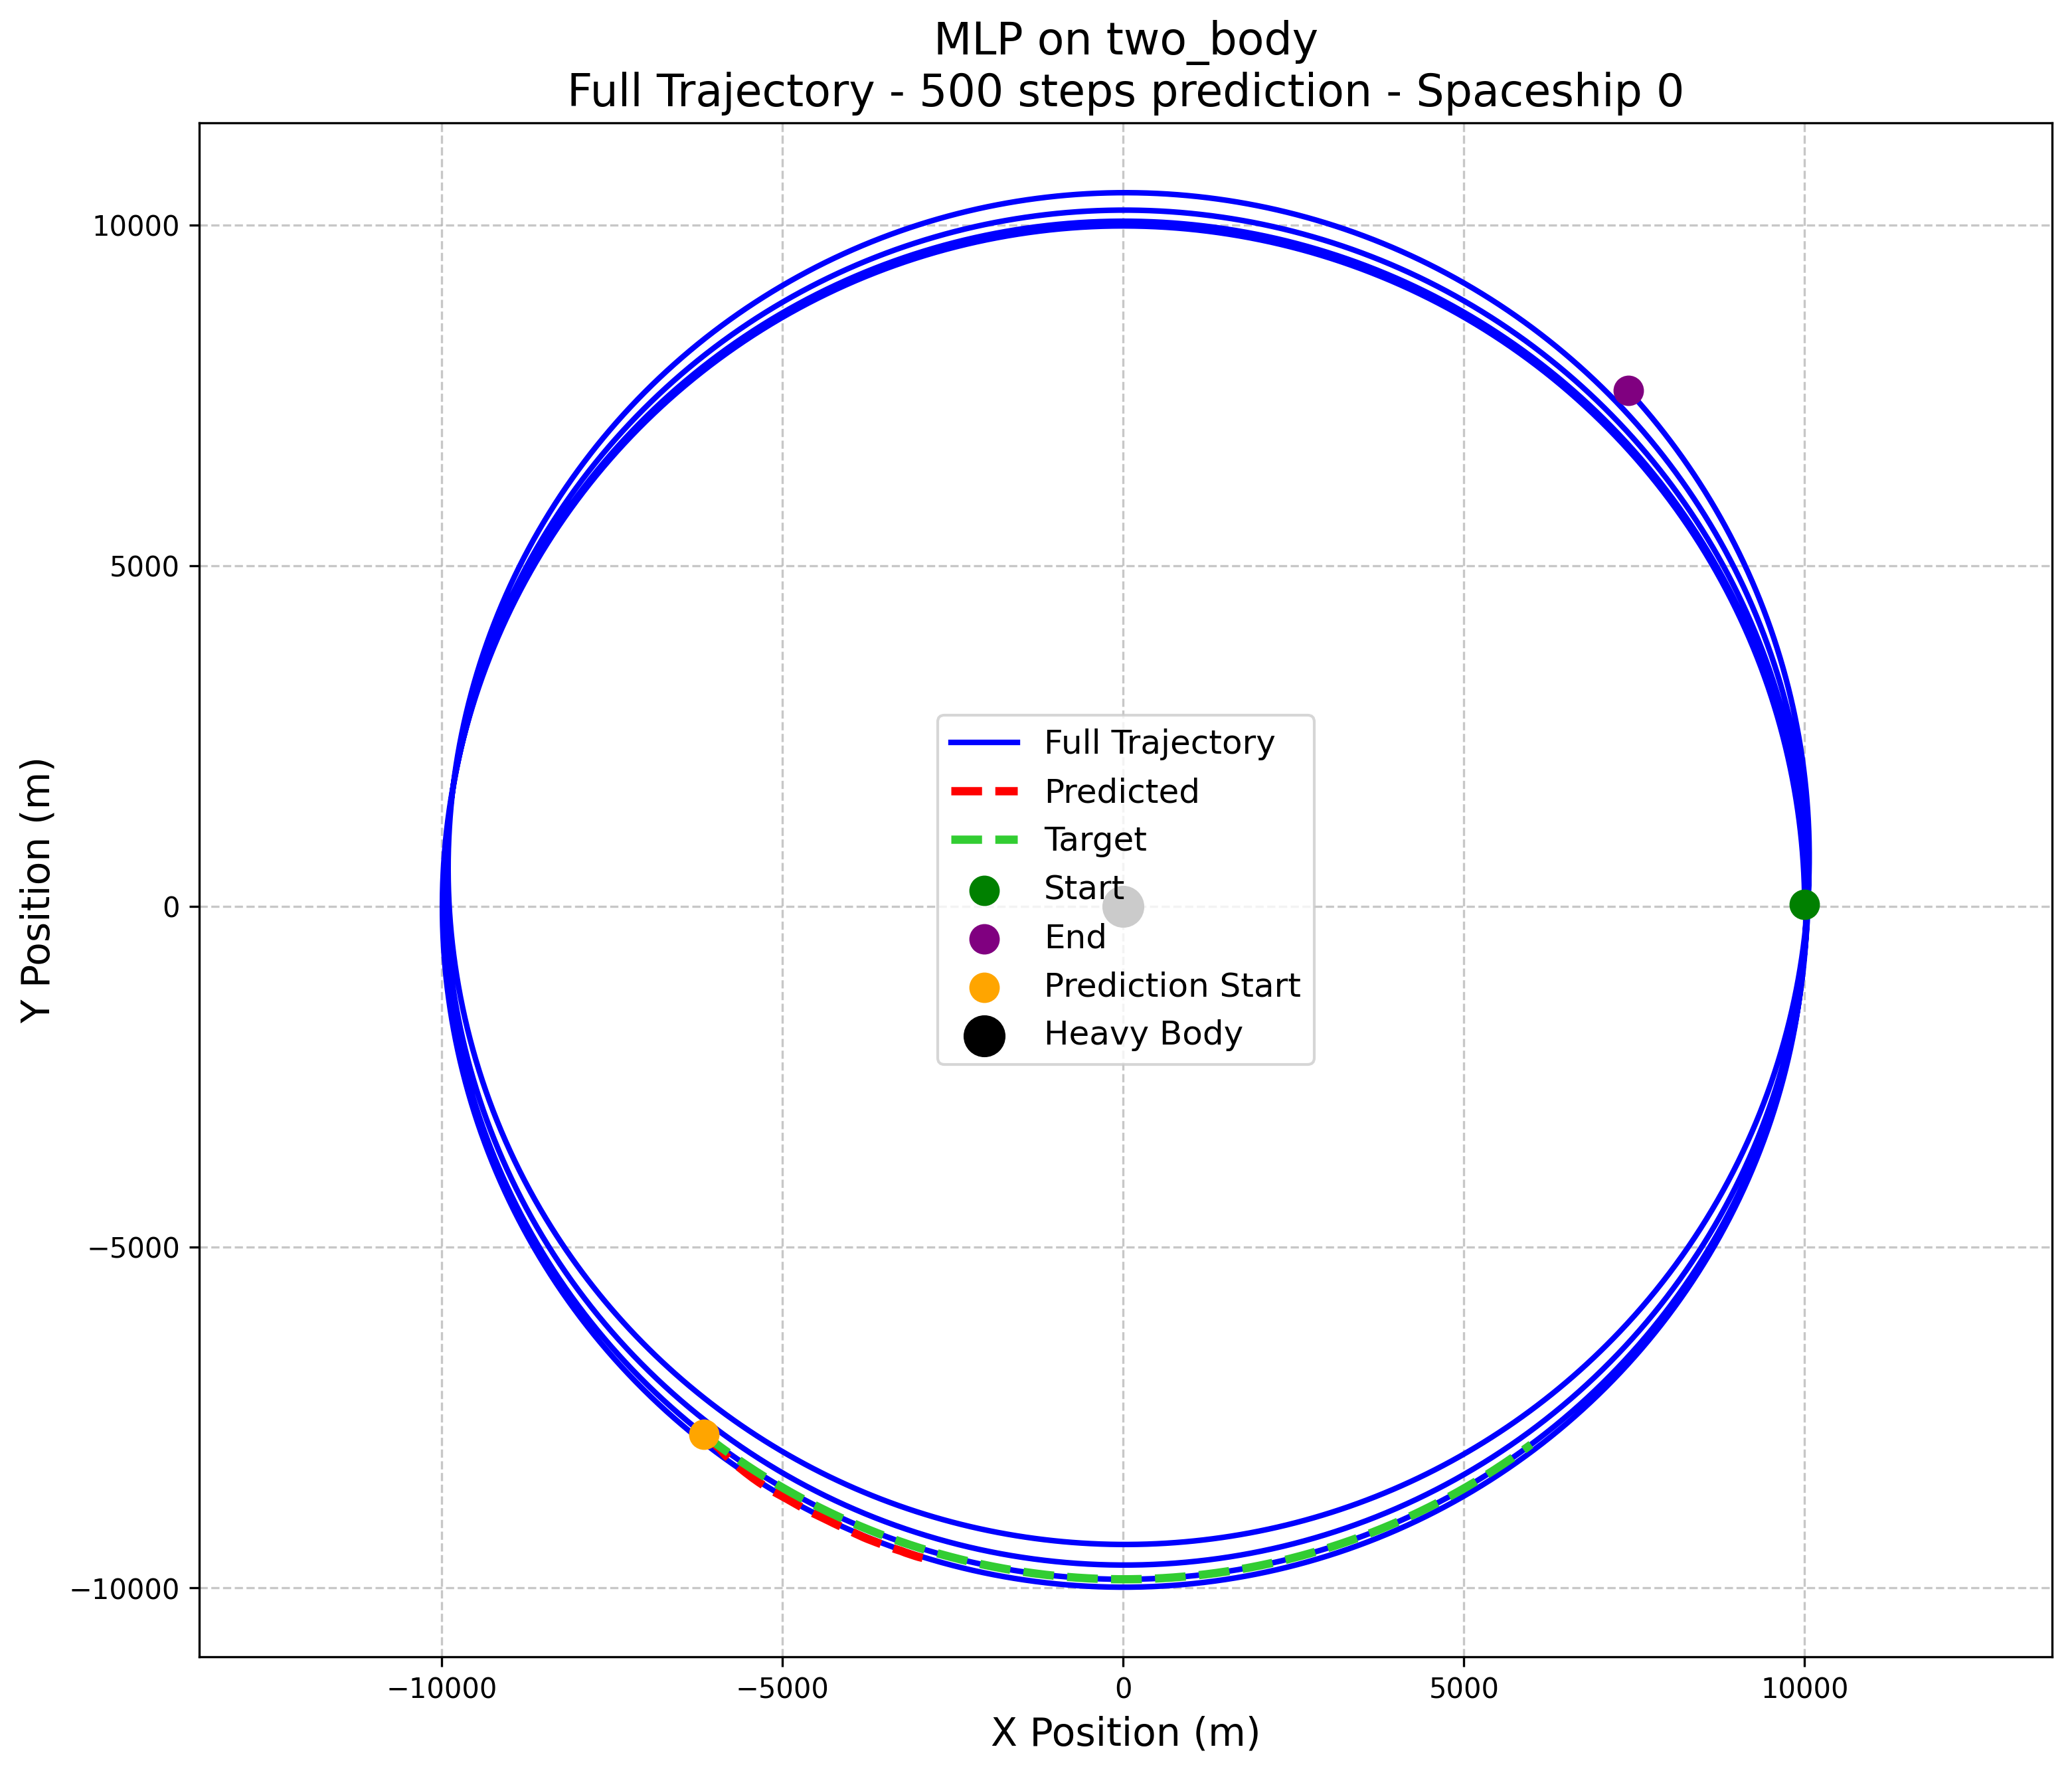
\includegraphics[width=0.27\textwidth]{../inference_results/train/MLP/two_body/500/full_trajectory_spaceship_0.png} &
      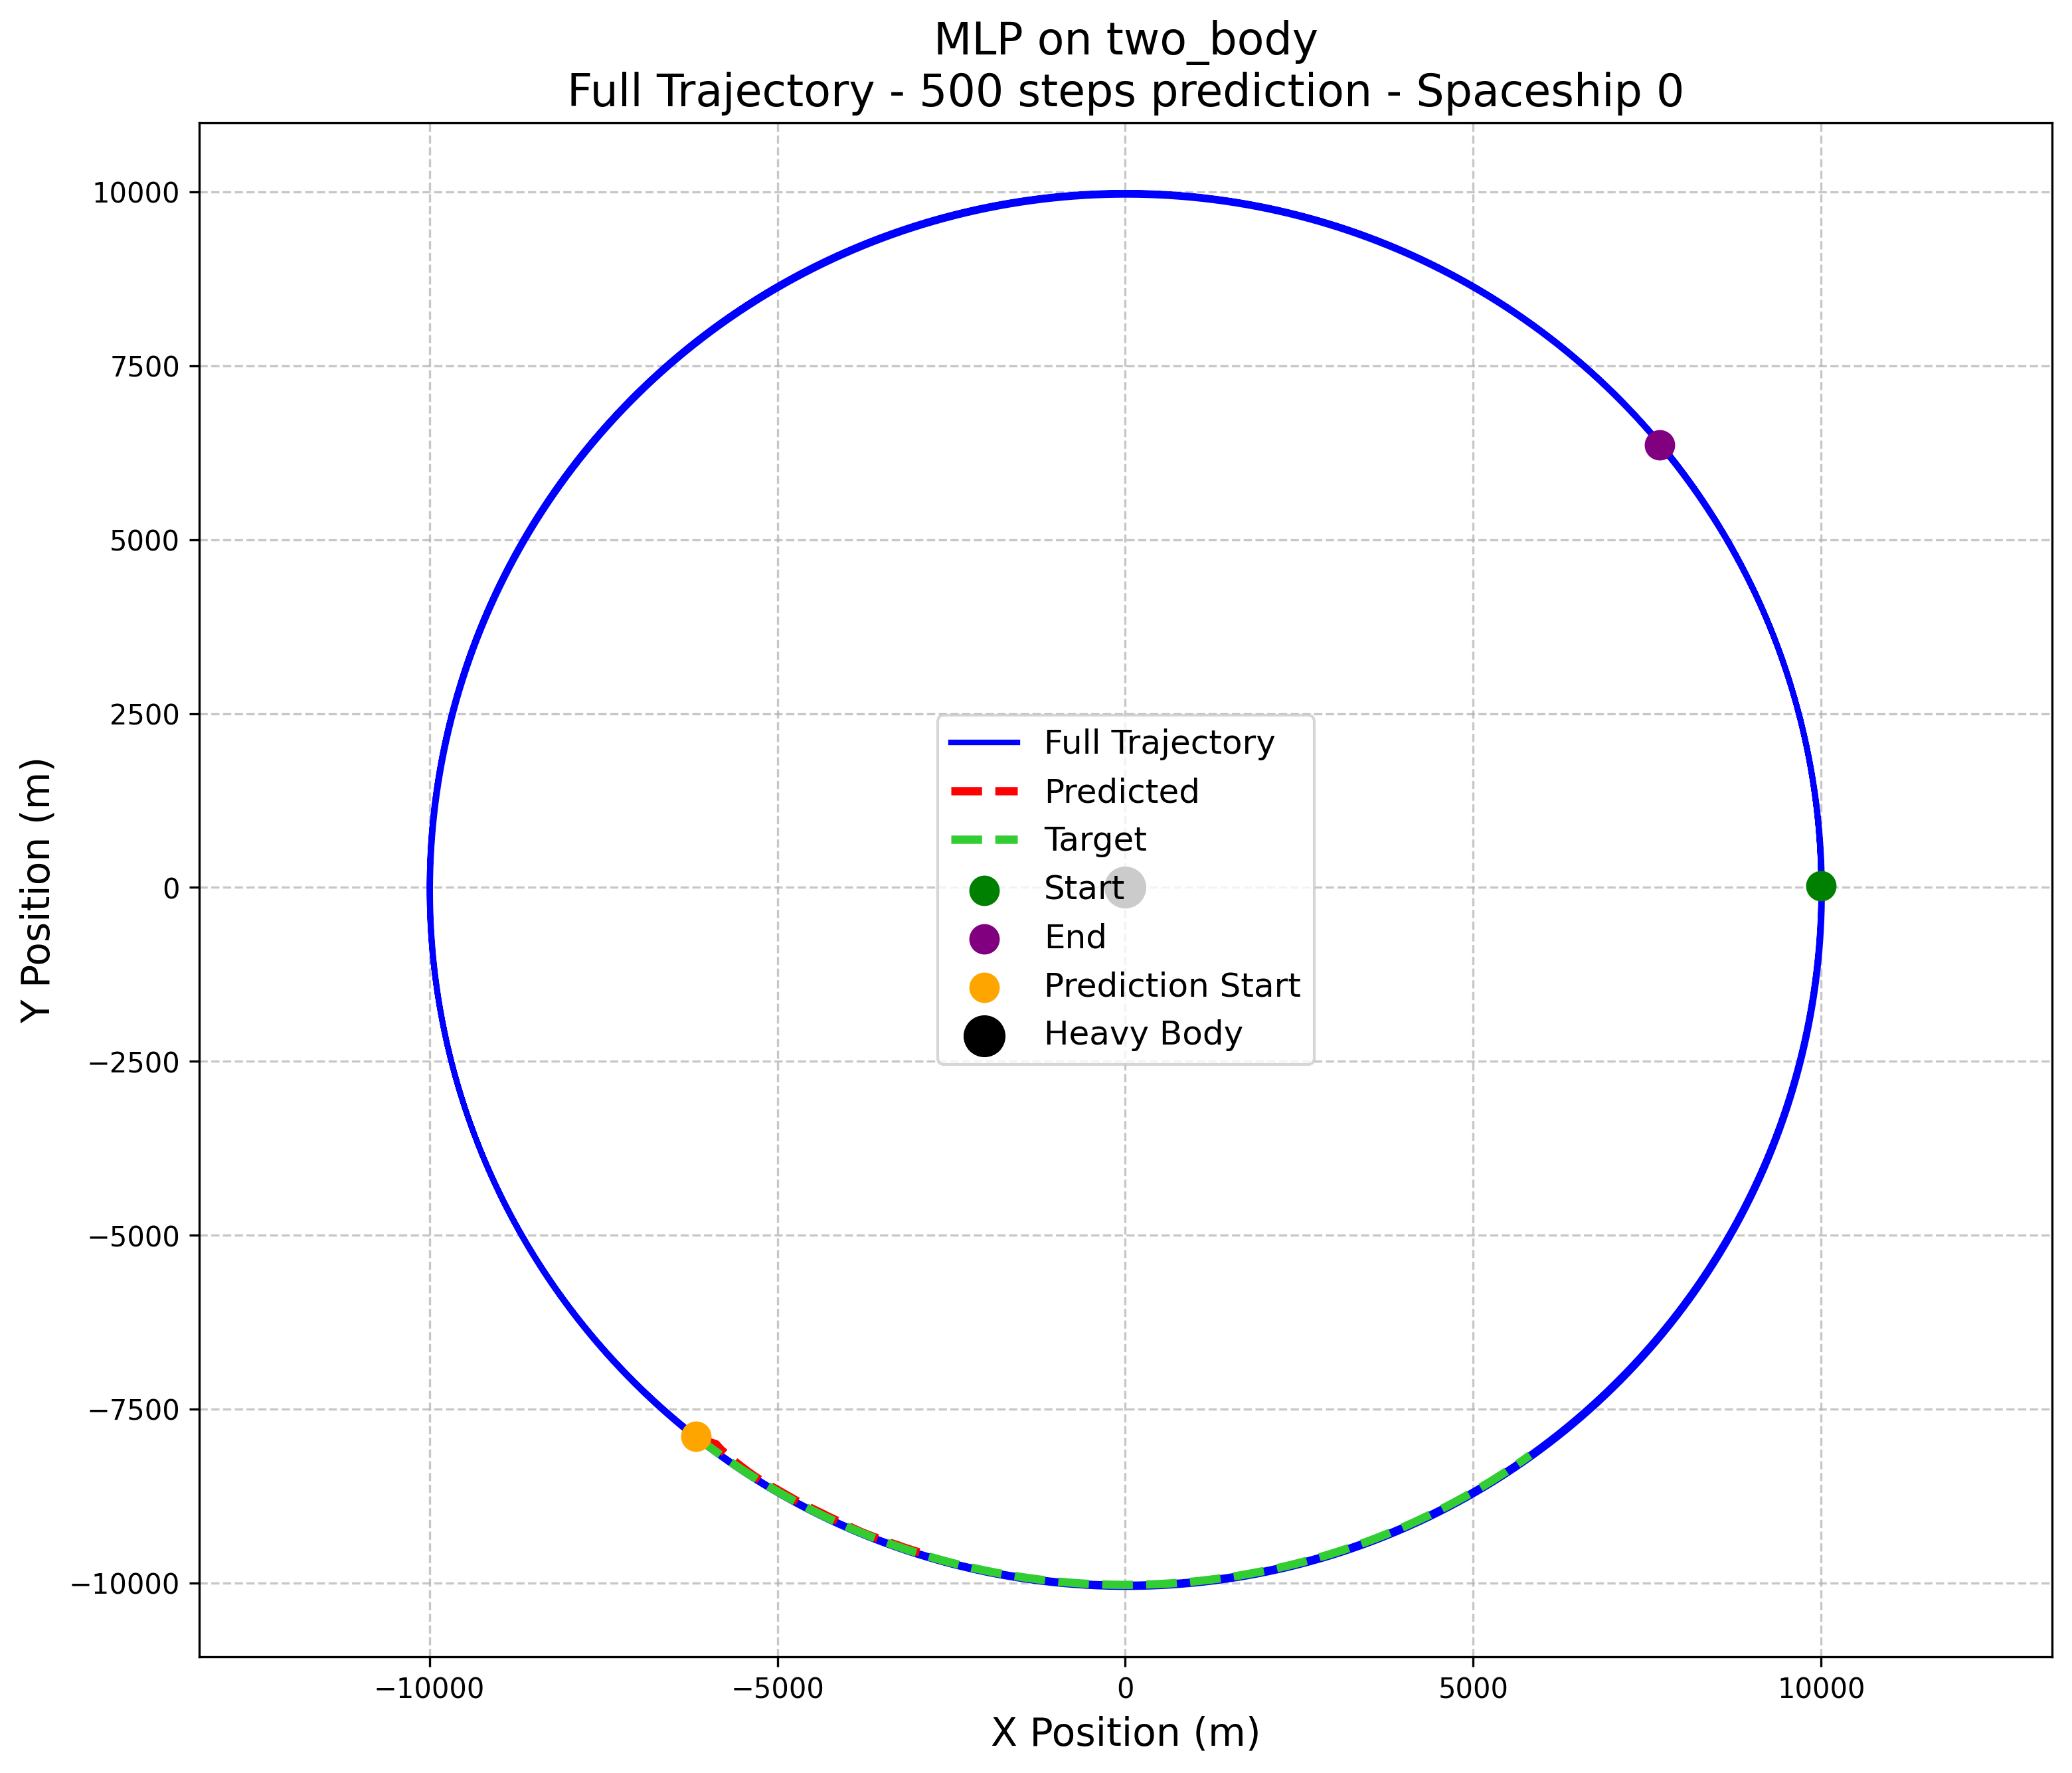
\includegraphics[width=0.27\textwidth]{../inference_results/val/MLP/two_body/500/full_trajectory_spaceship_0.png} &
      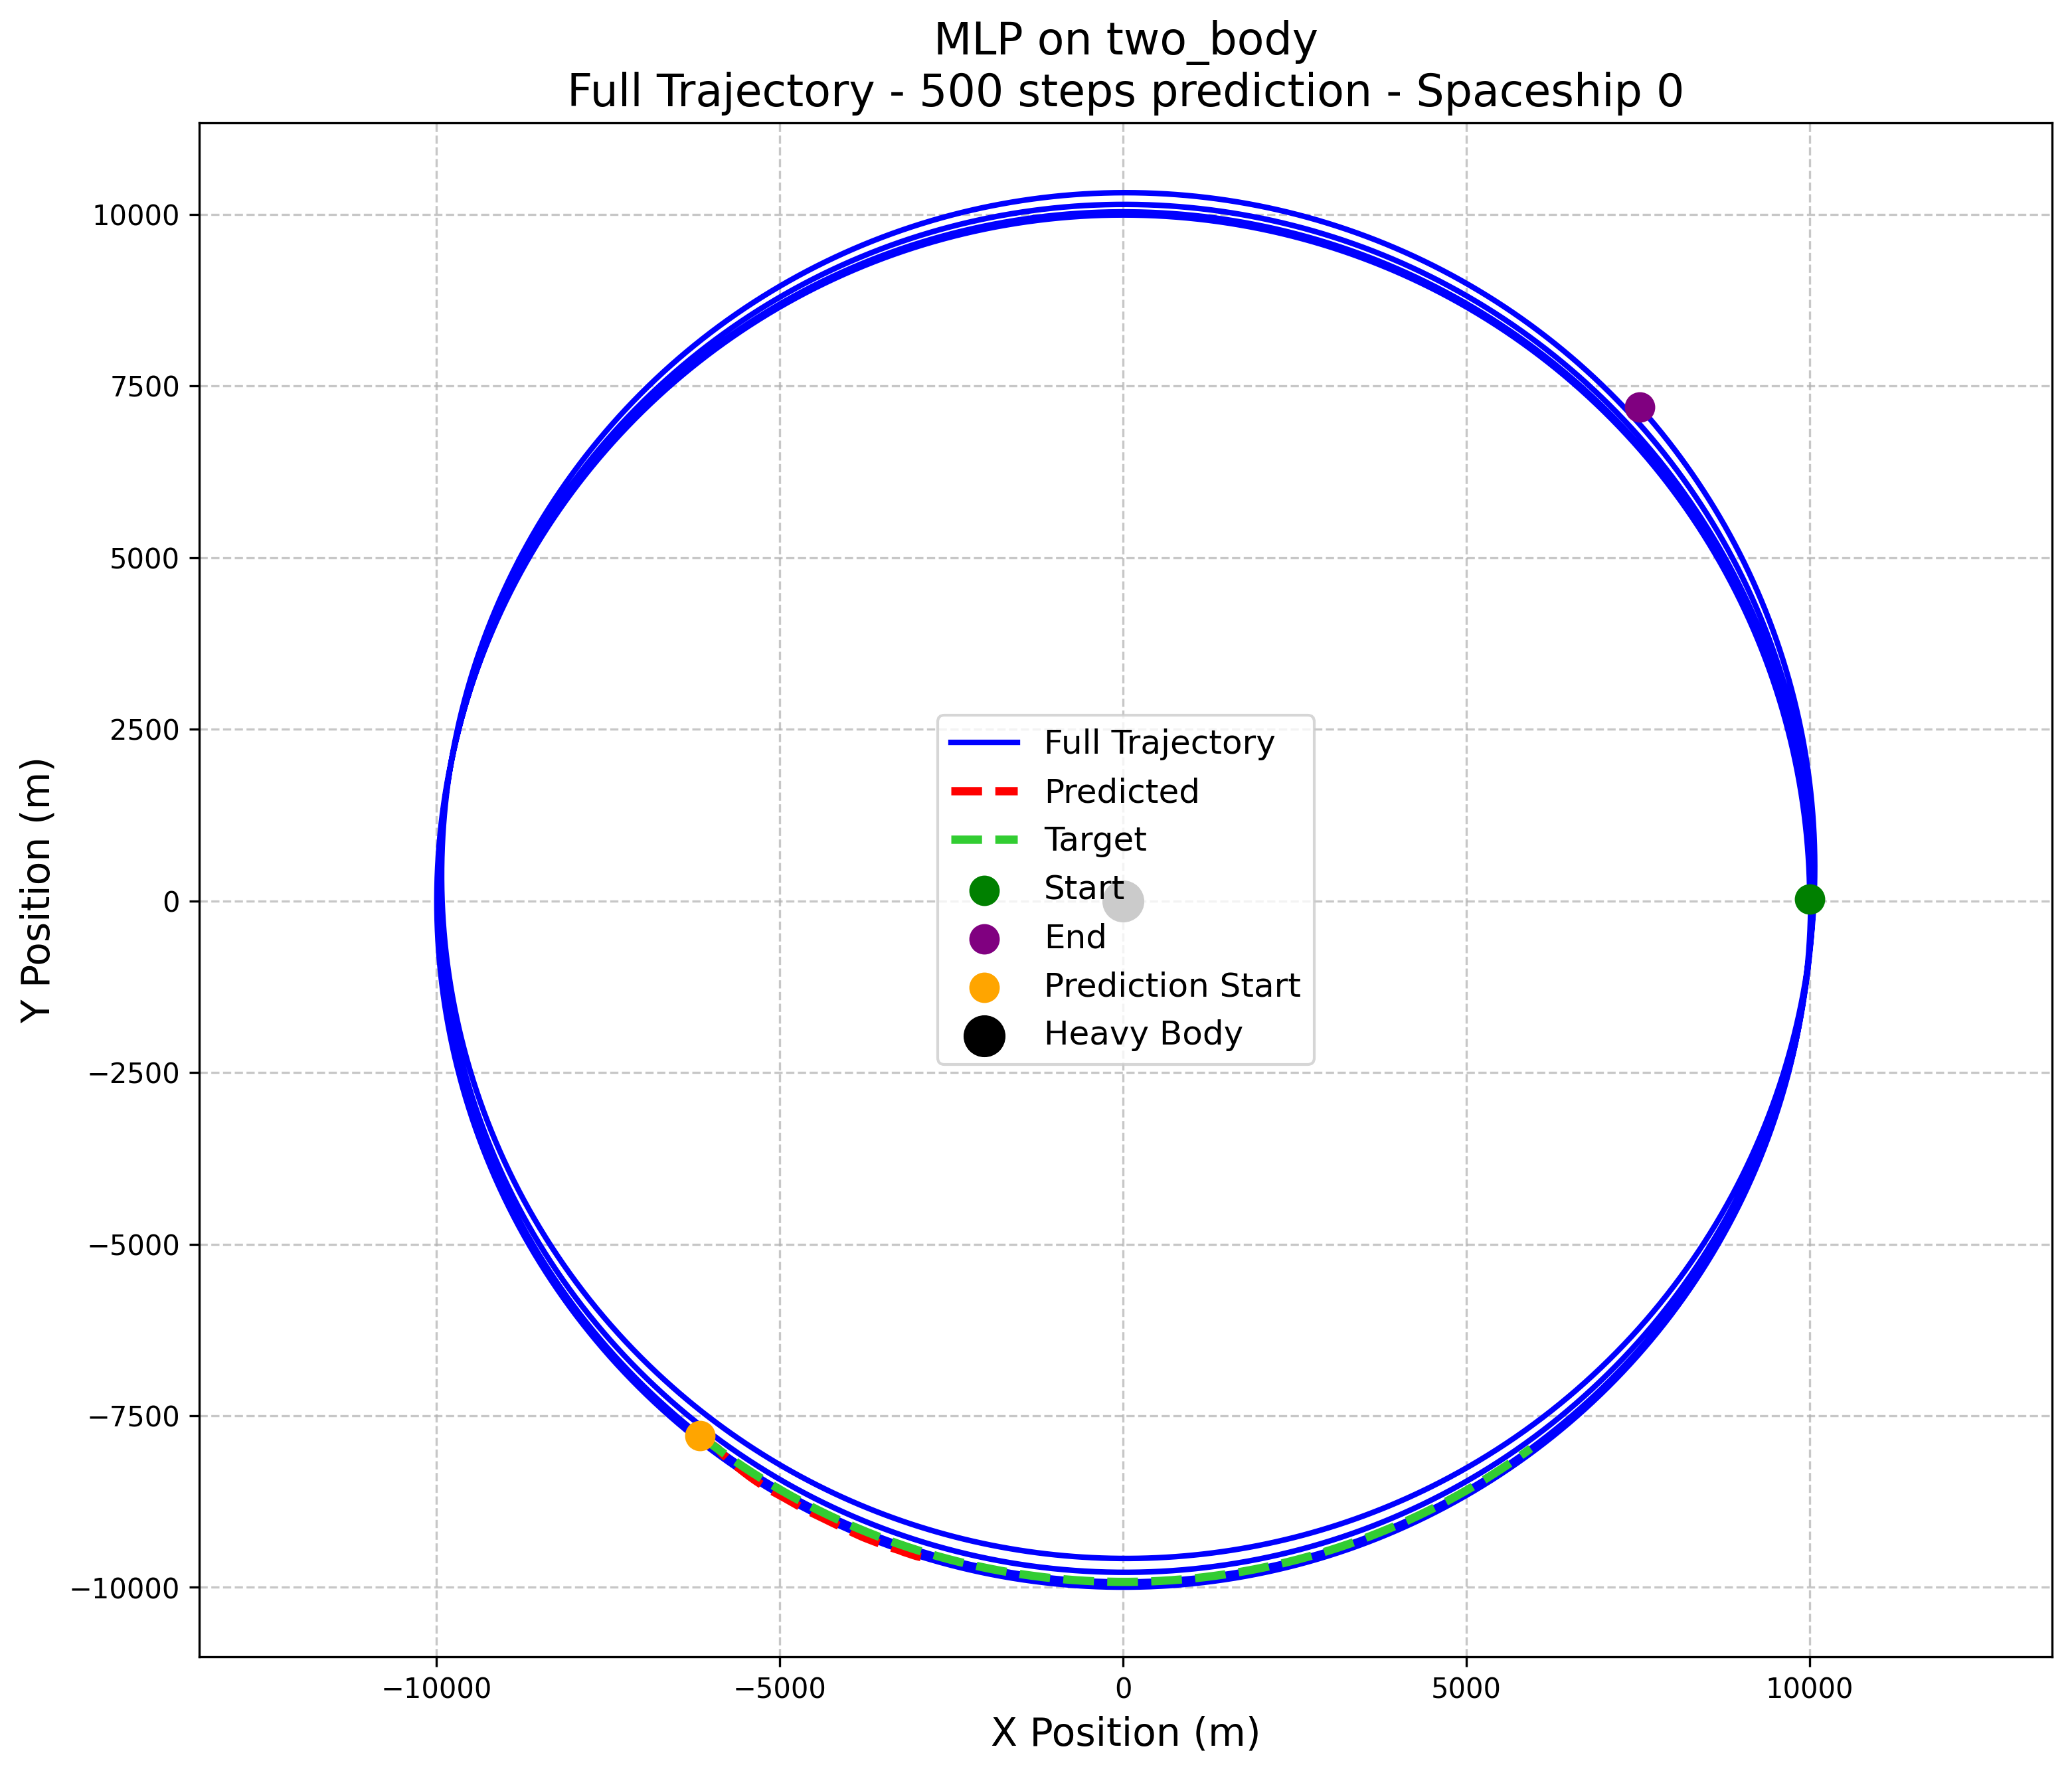
\includegraphics[width=0.27\textwidth]{../inference_results/test/MLP/two_body/500/full_trajectory_spaceship_0.png} \\
      LSTM &
      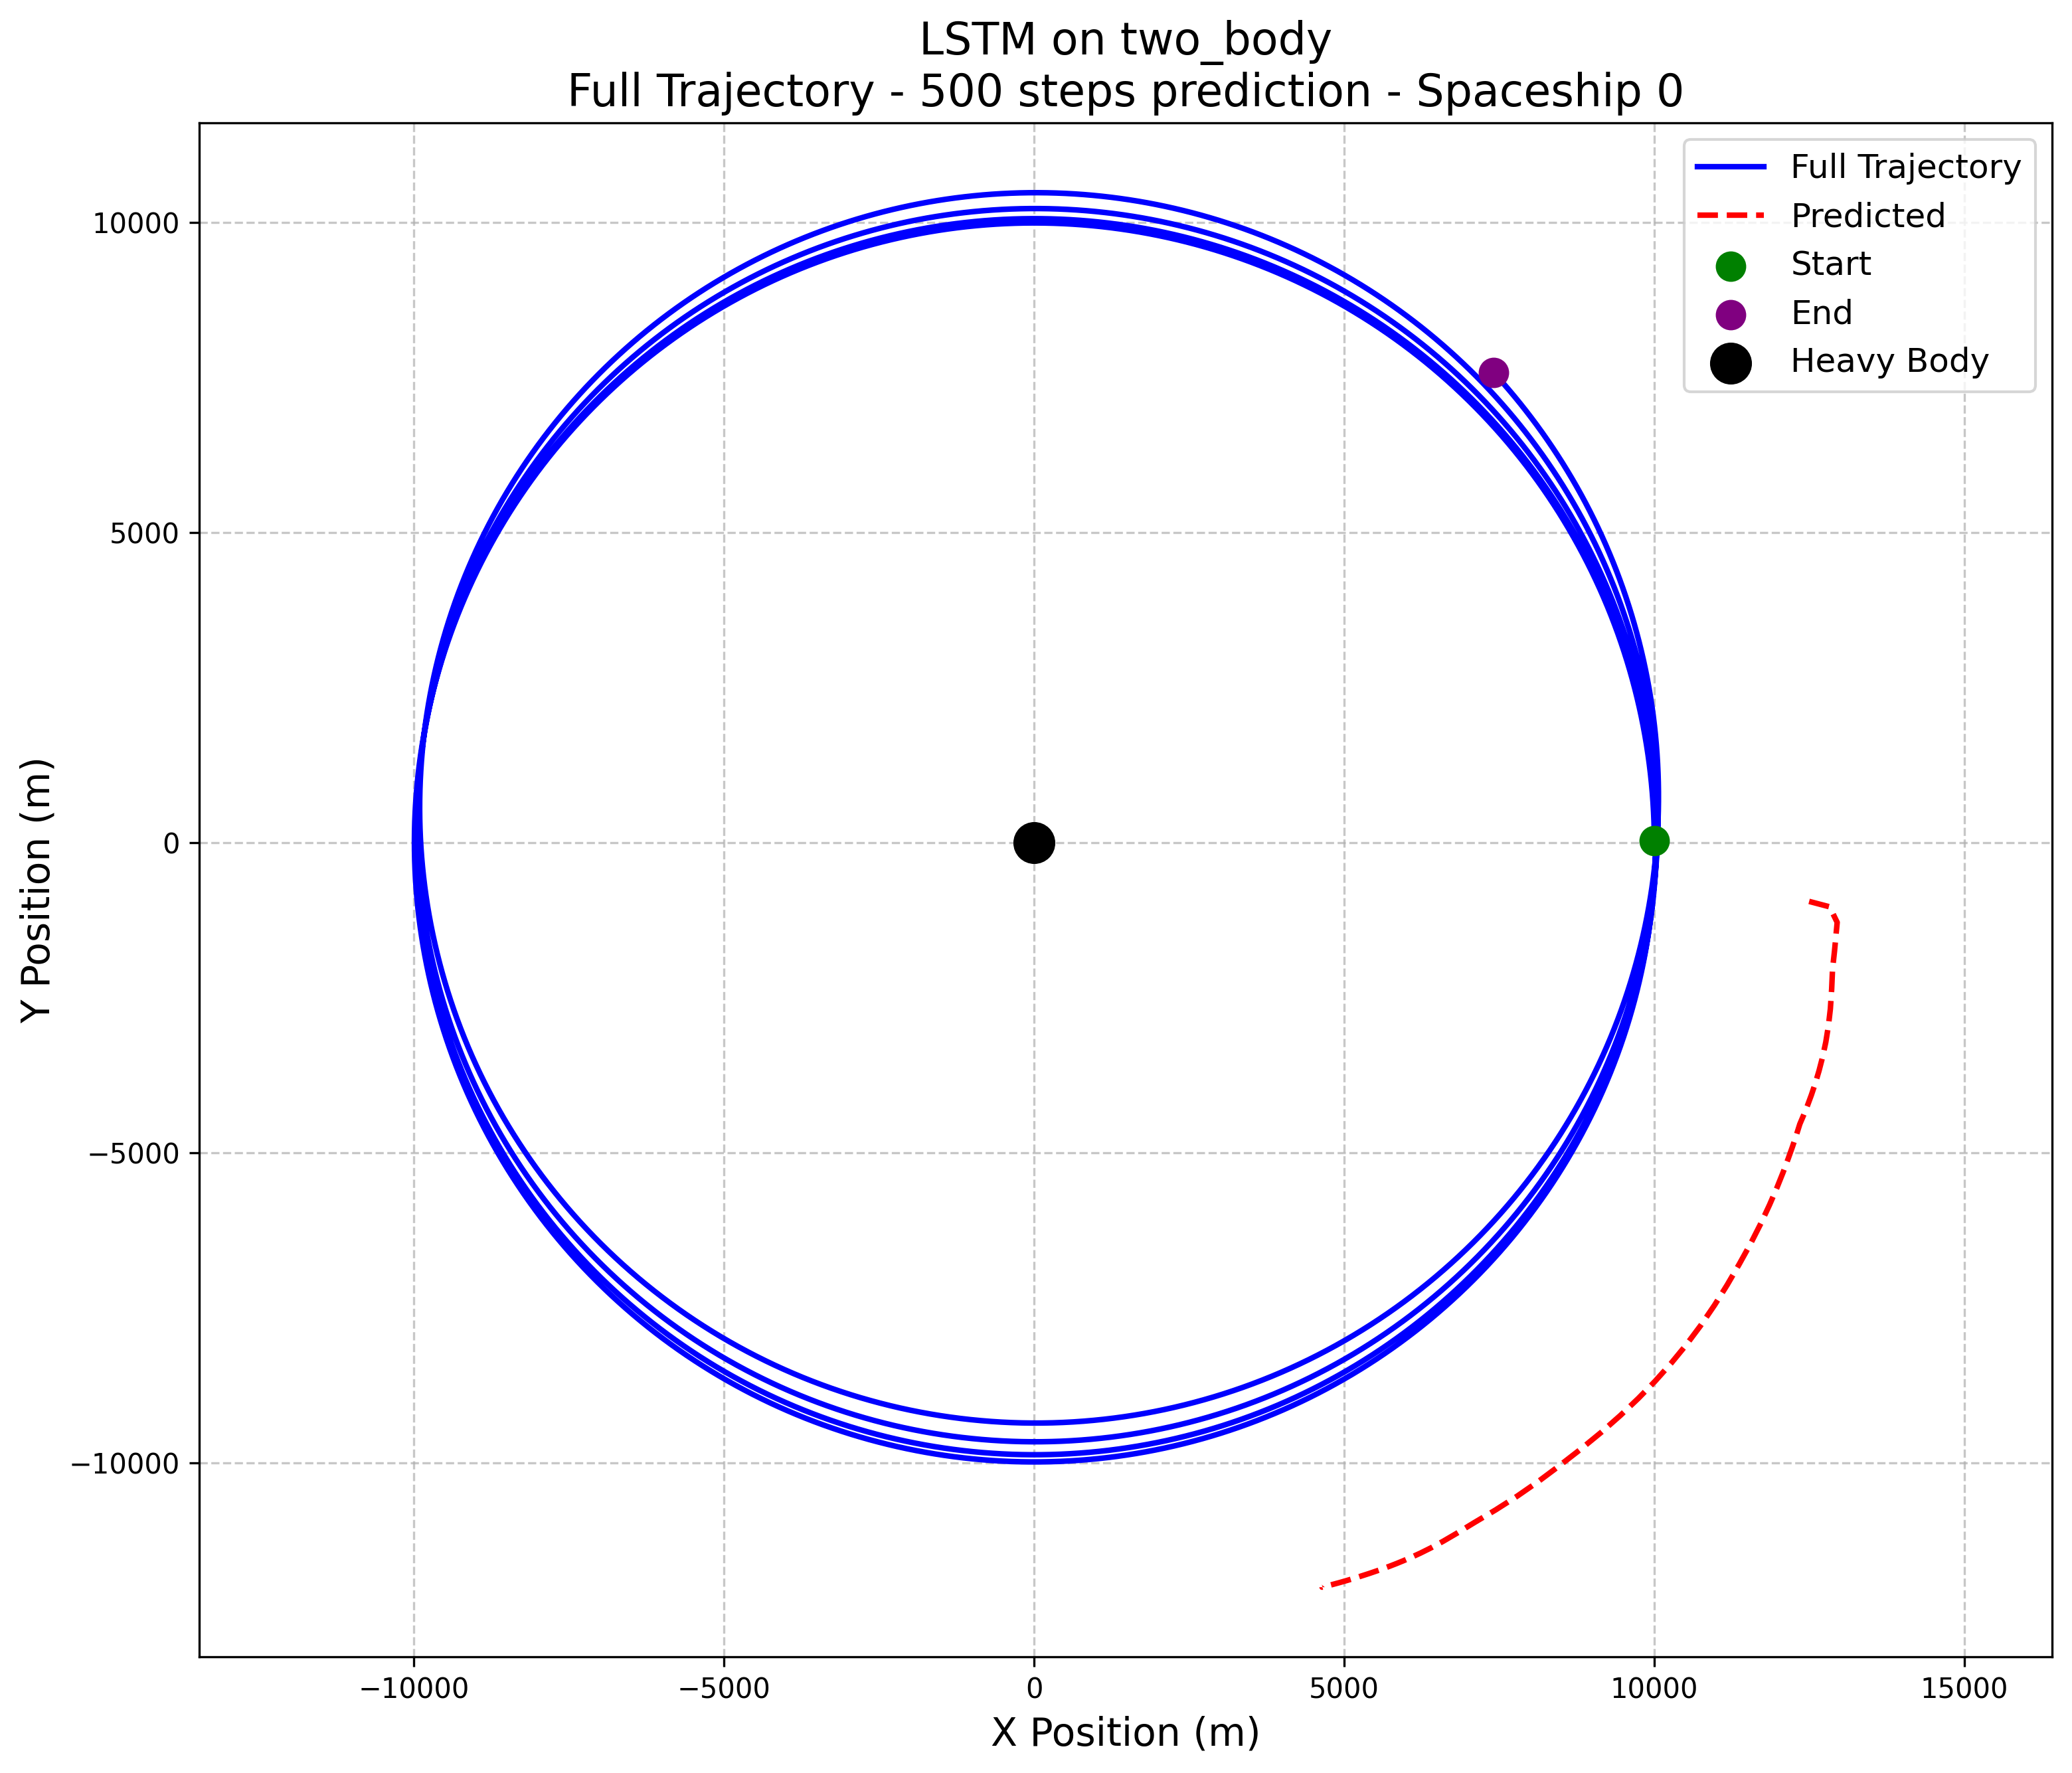
\includegraphics[width=0.27\textwidth]{../inference_results/train/LSTM/two_body/500/full_trajectory_spaceship_0.png} &
      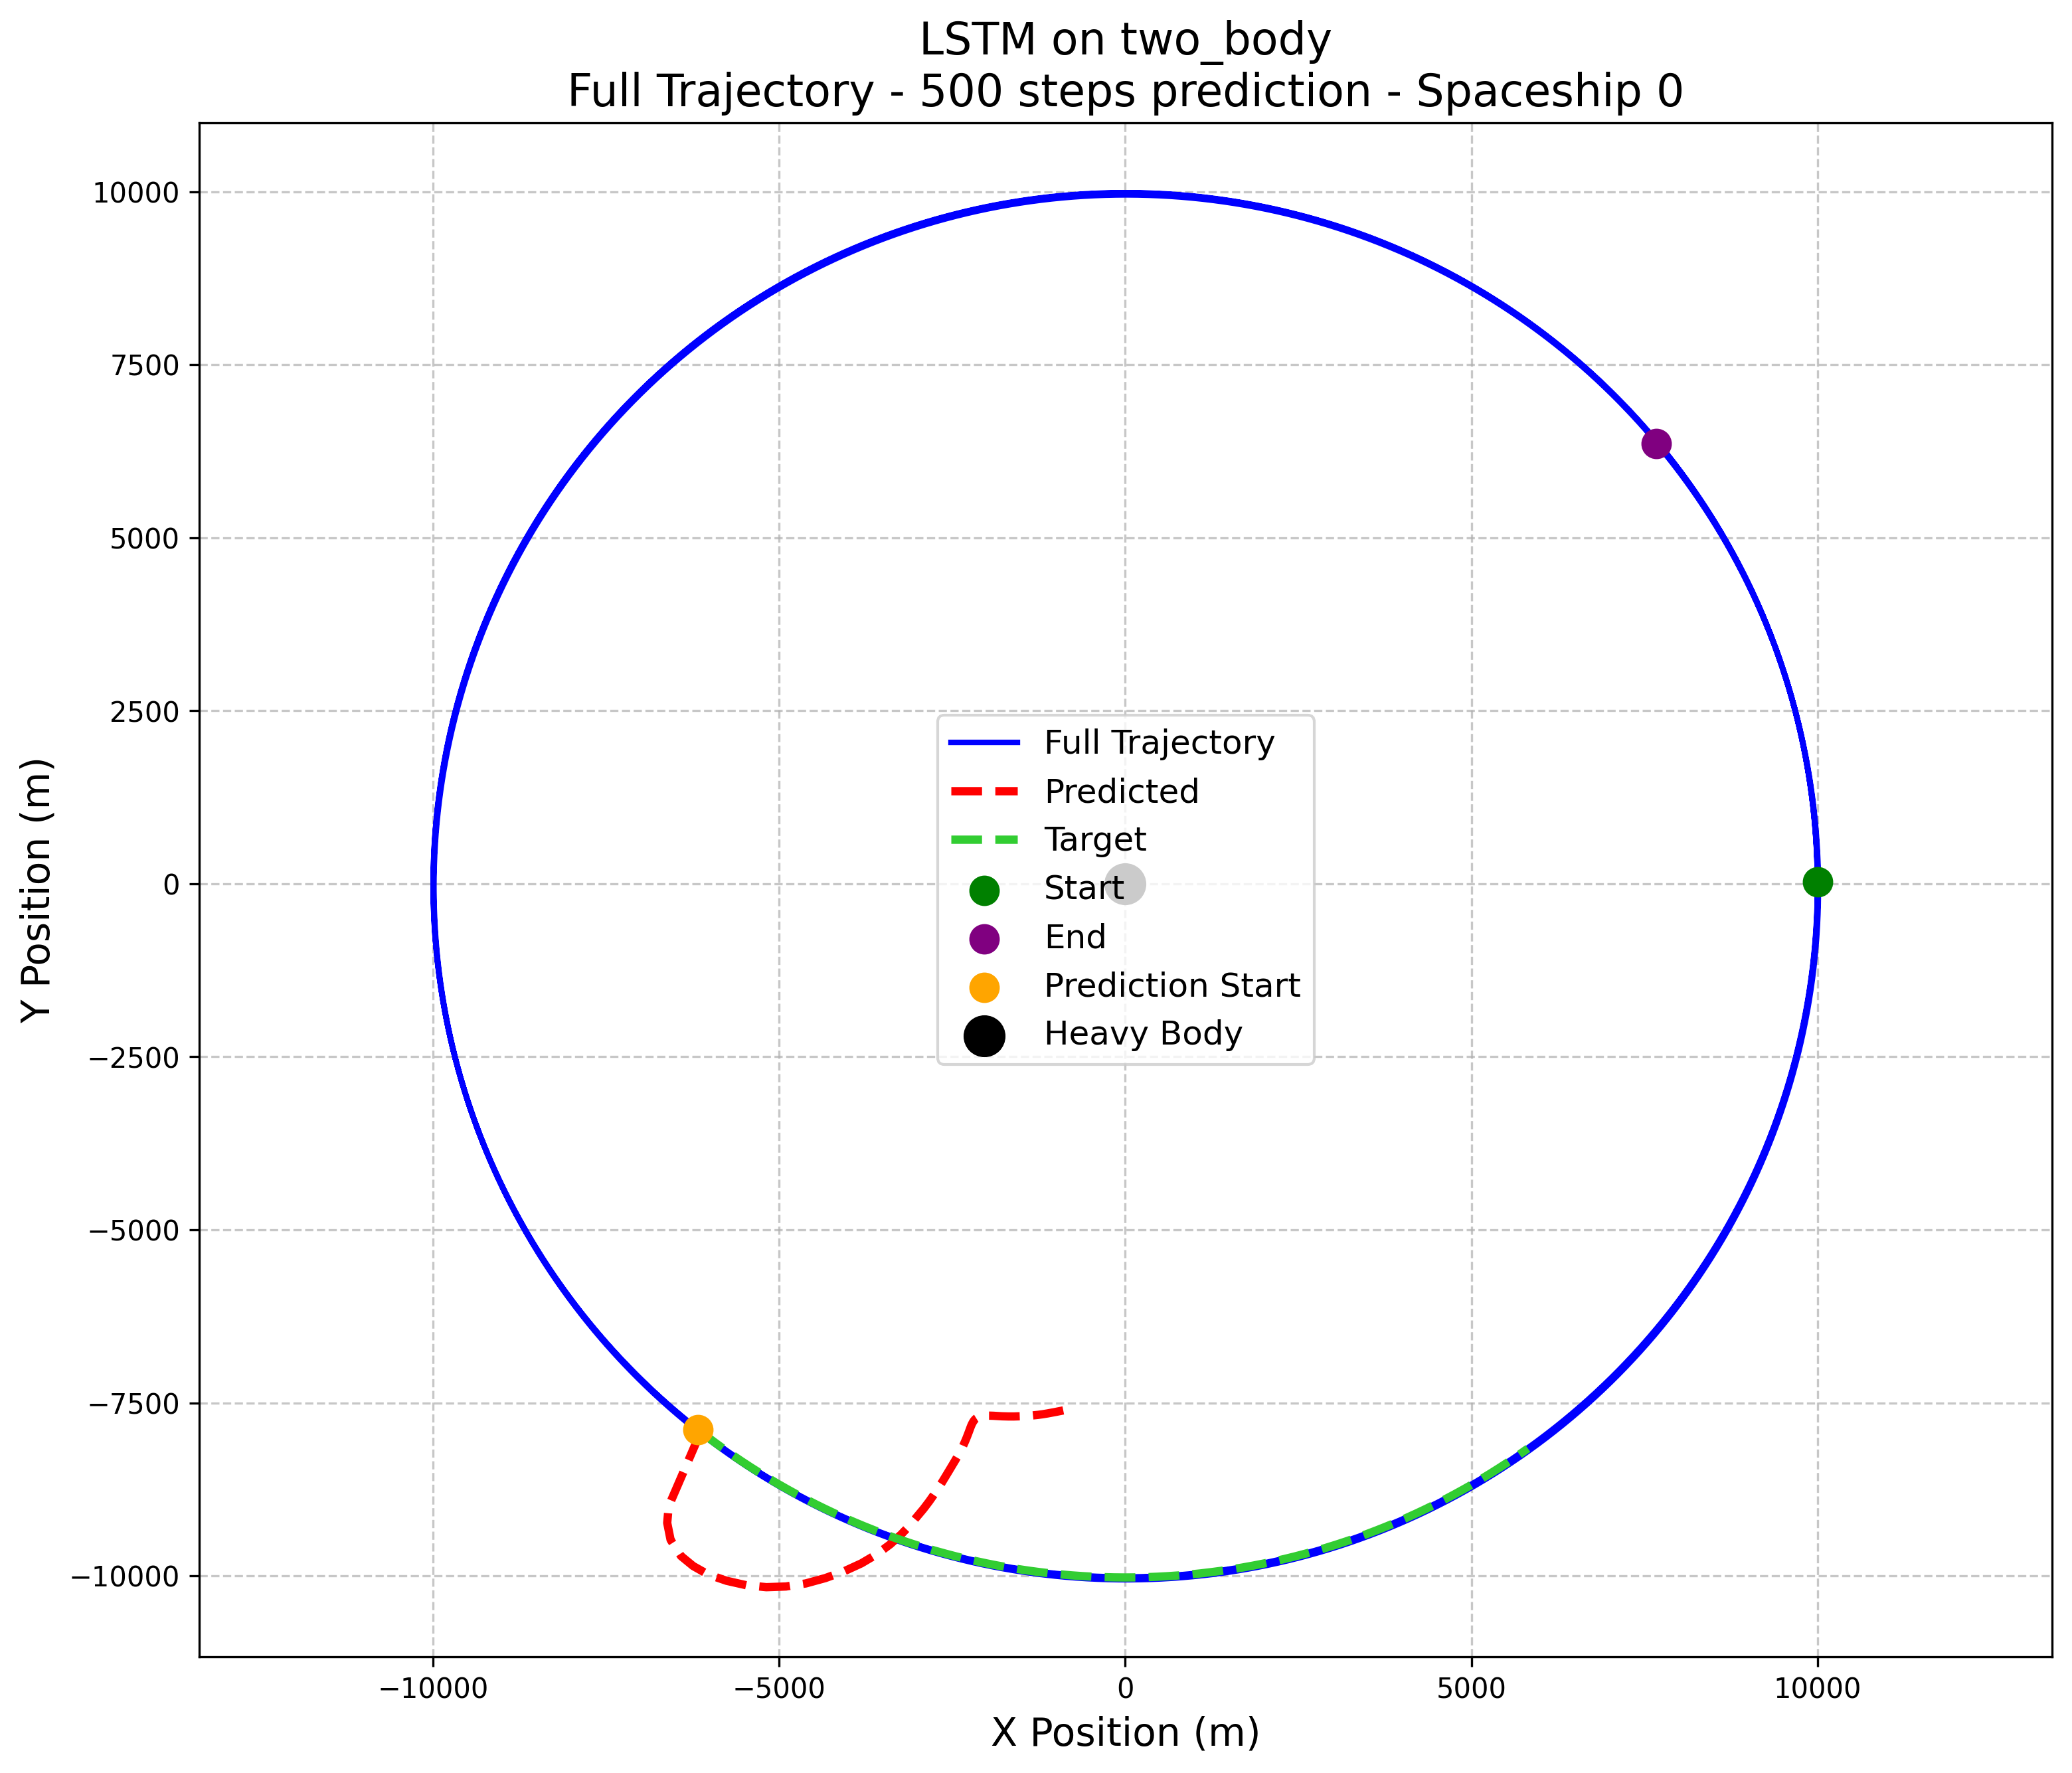
\includegraphics[width=0.27\textwidth]{../inference_results/val/LSTM/two_body/500/full_trajectory_spaceship_0.png} &
      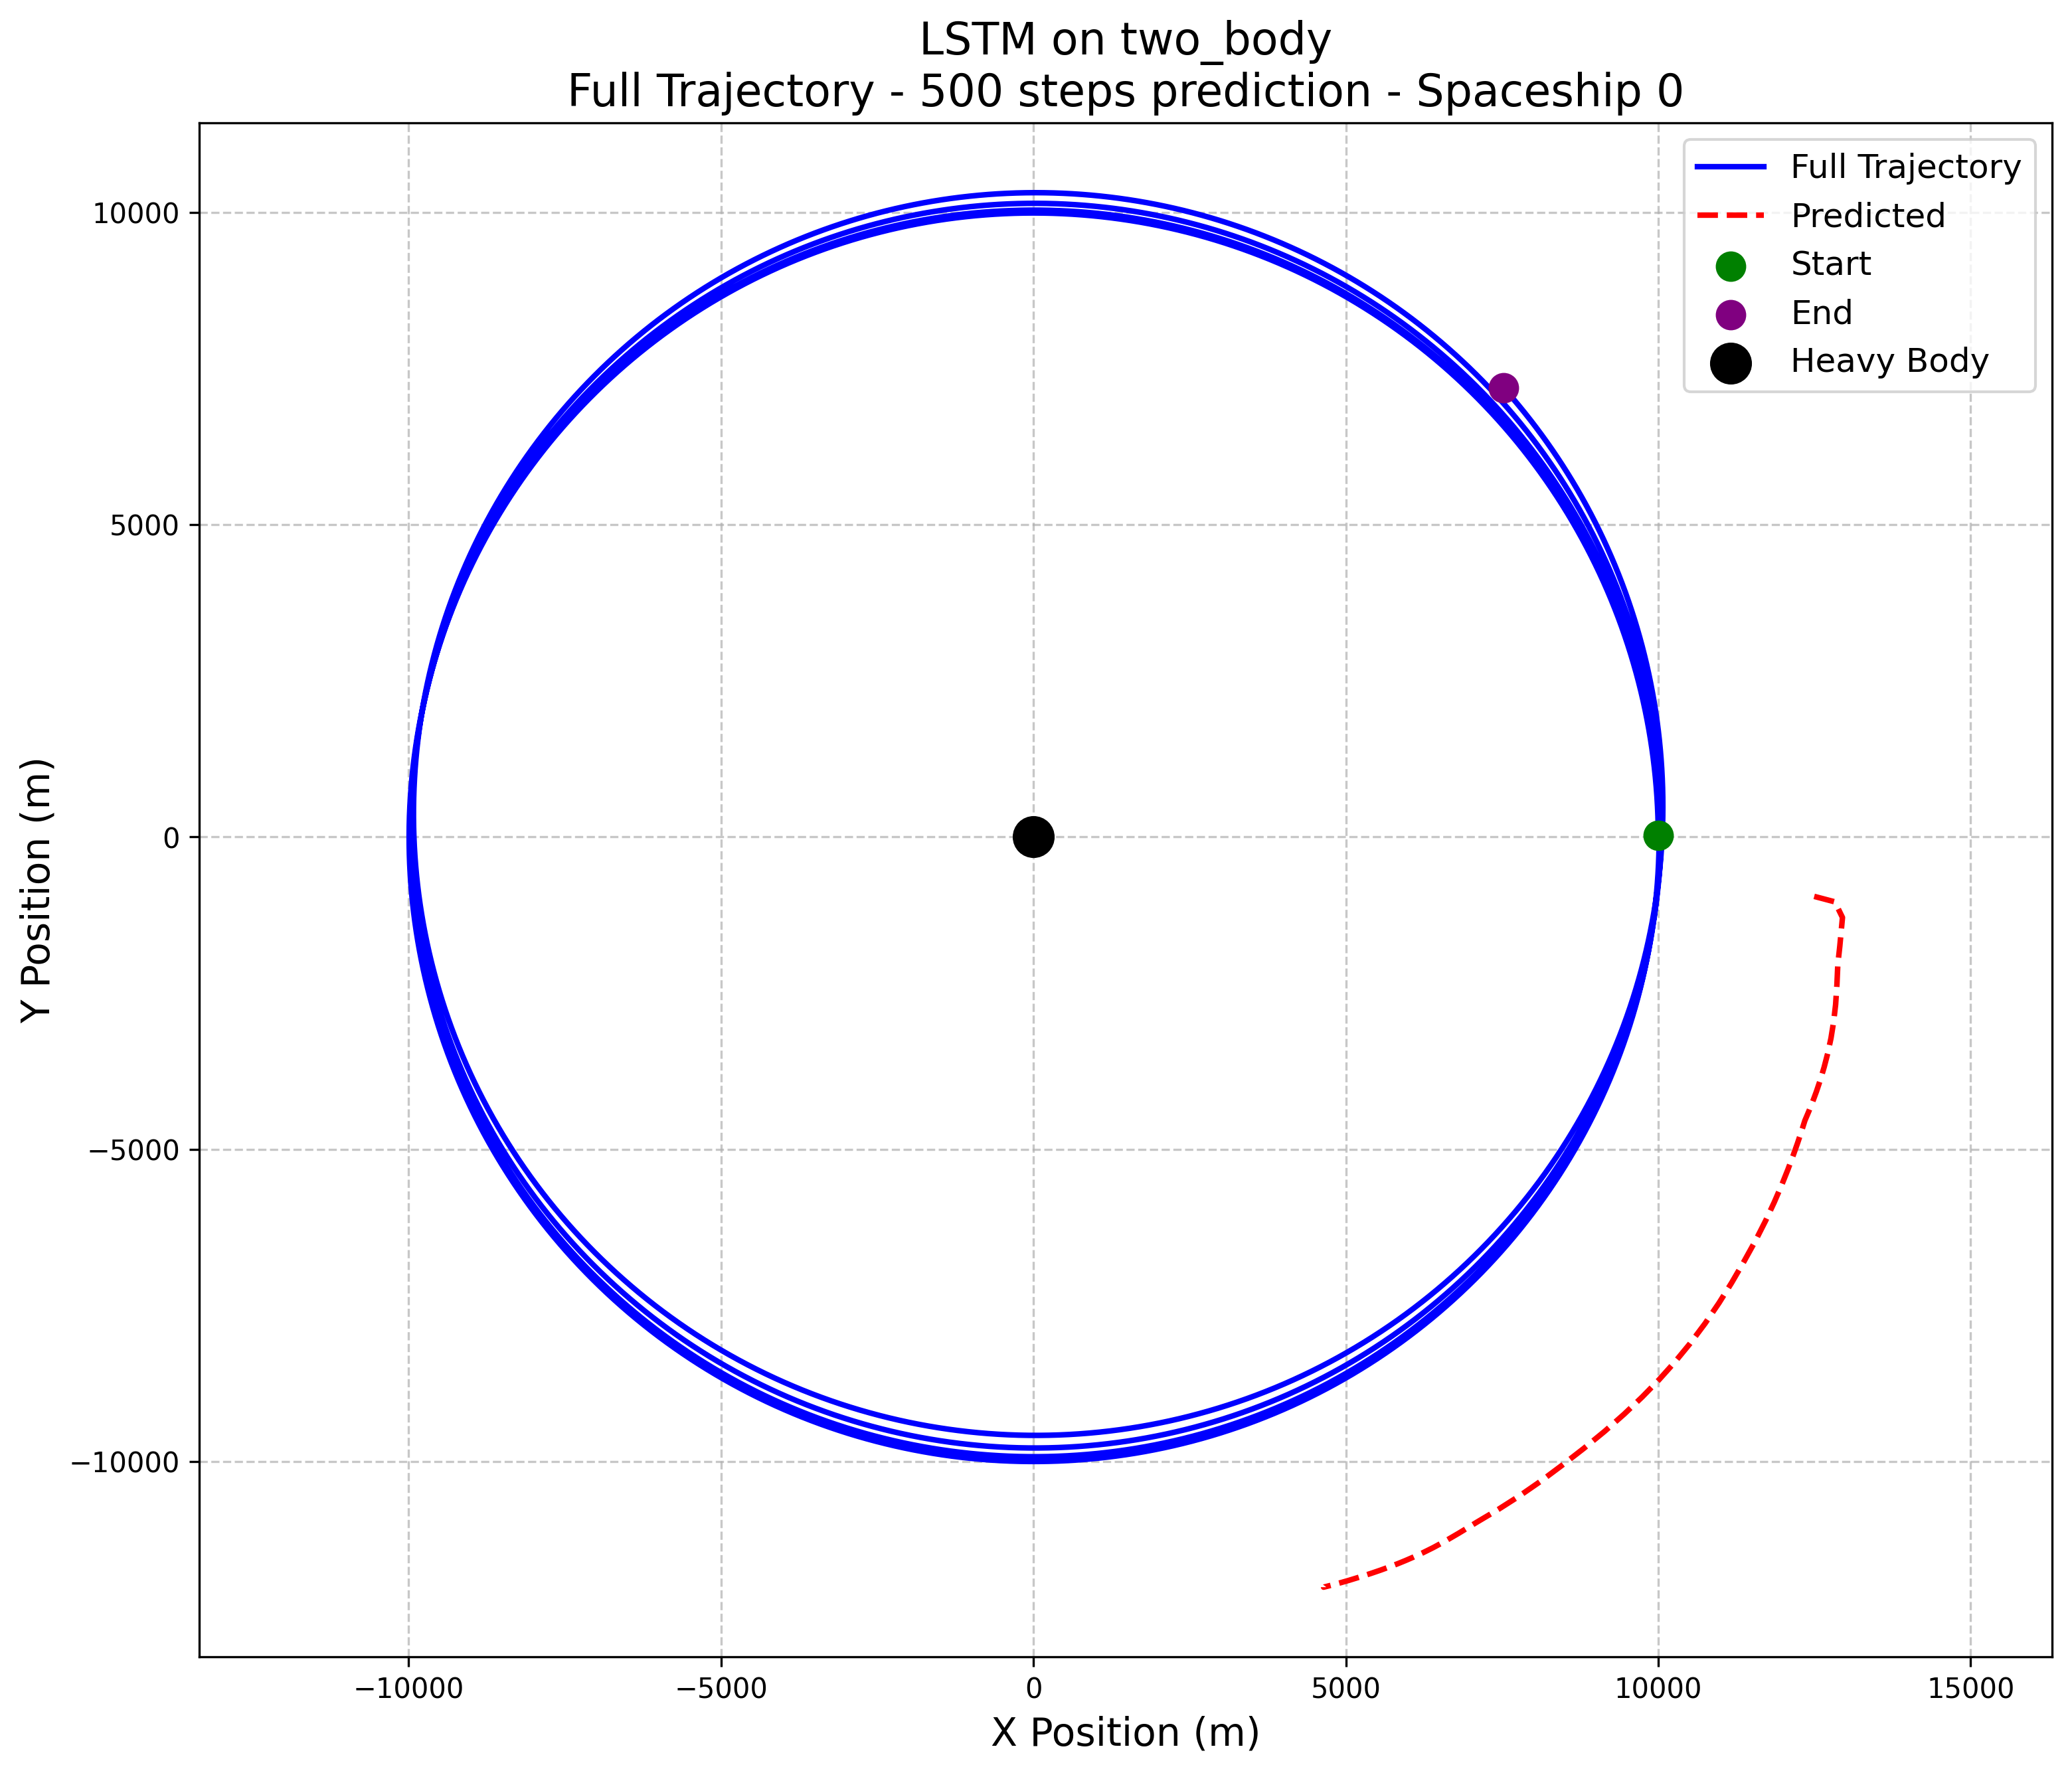
\includegraphics[width=0.27\textwidth]{../inference_results/test/LSTM/two_body/500/full_trajectory_spaceship_0.png} \\
      PINN &
      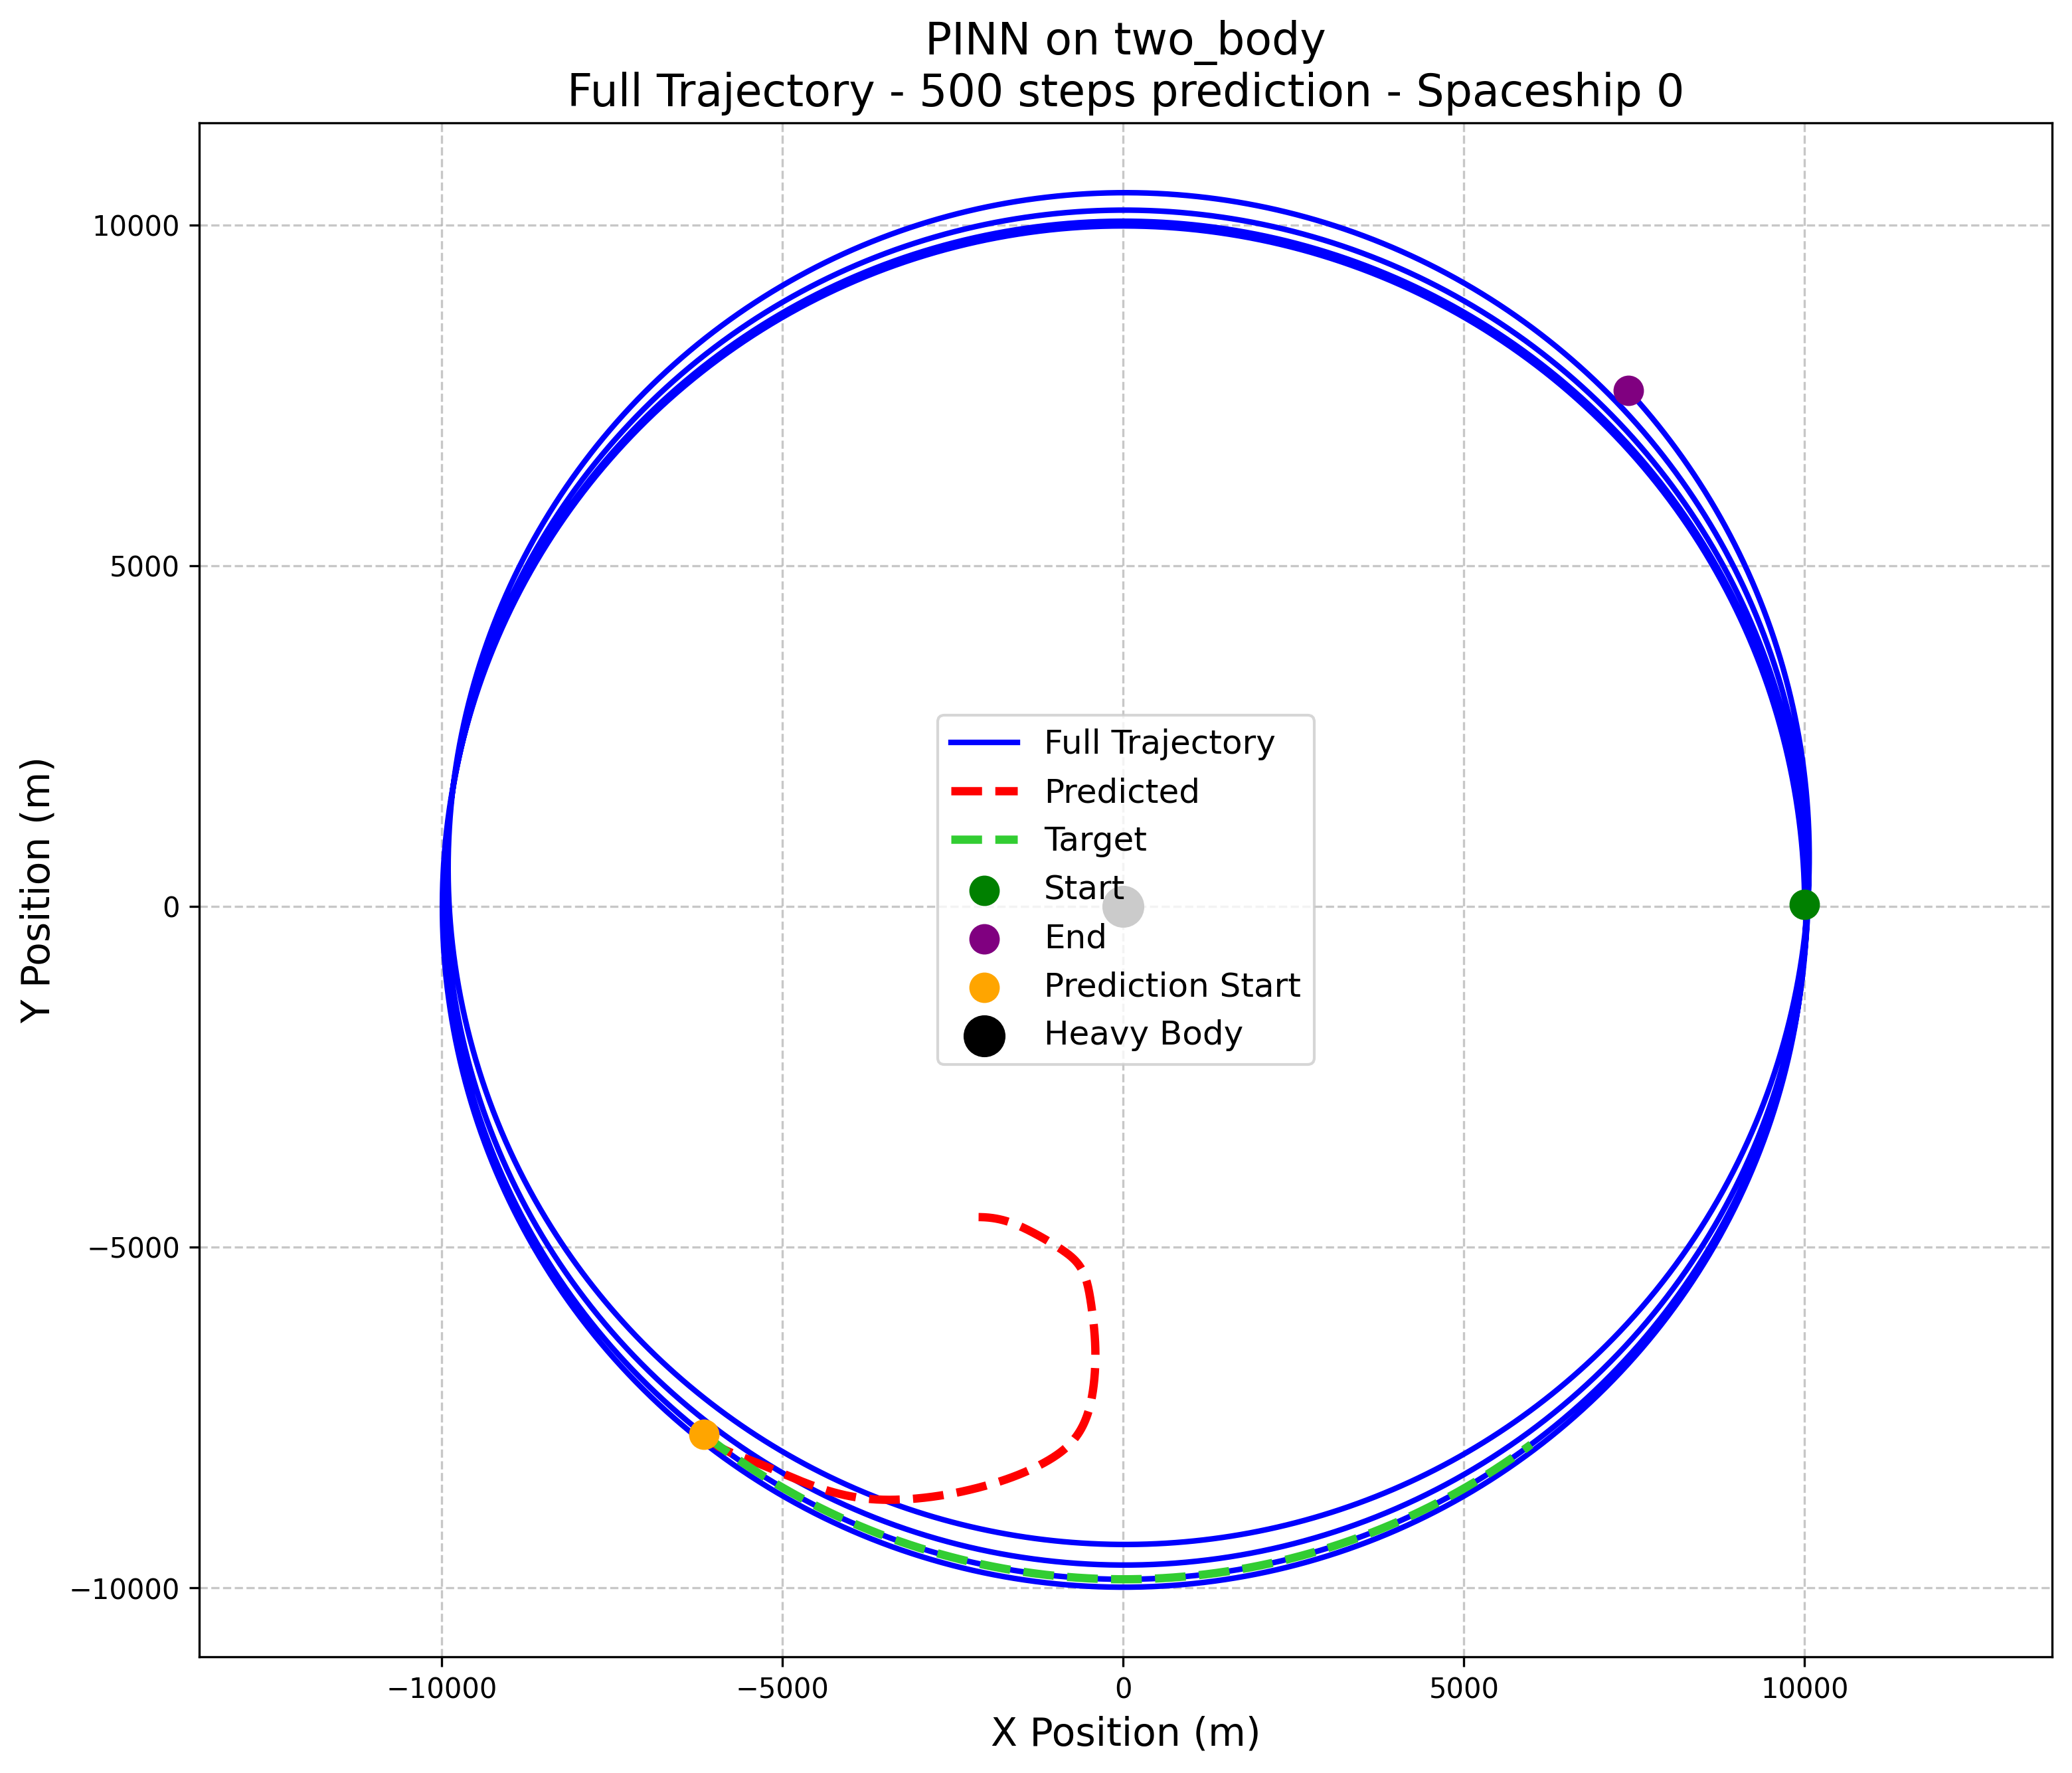
\includegraphics[width=0.27\textwidth]{../inference_results/train/PINN/two_body/500/full_trajectory_spaceship_0.png} &
      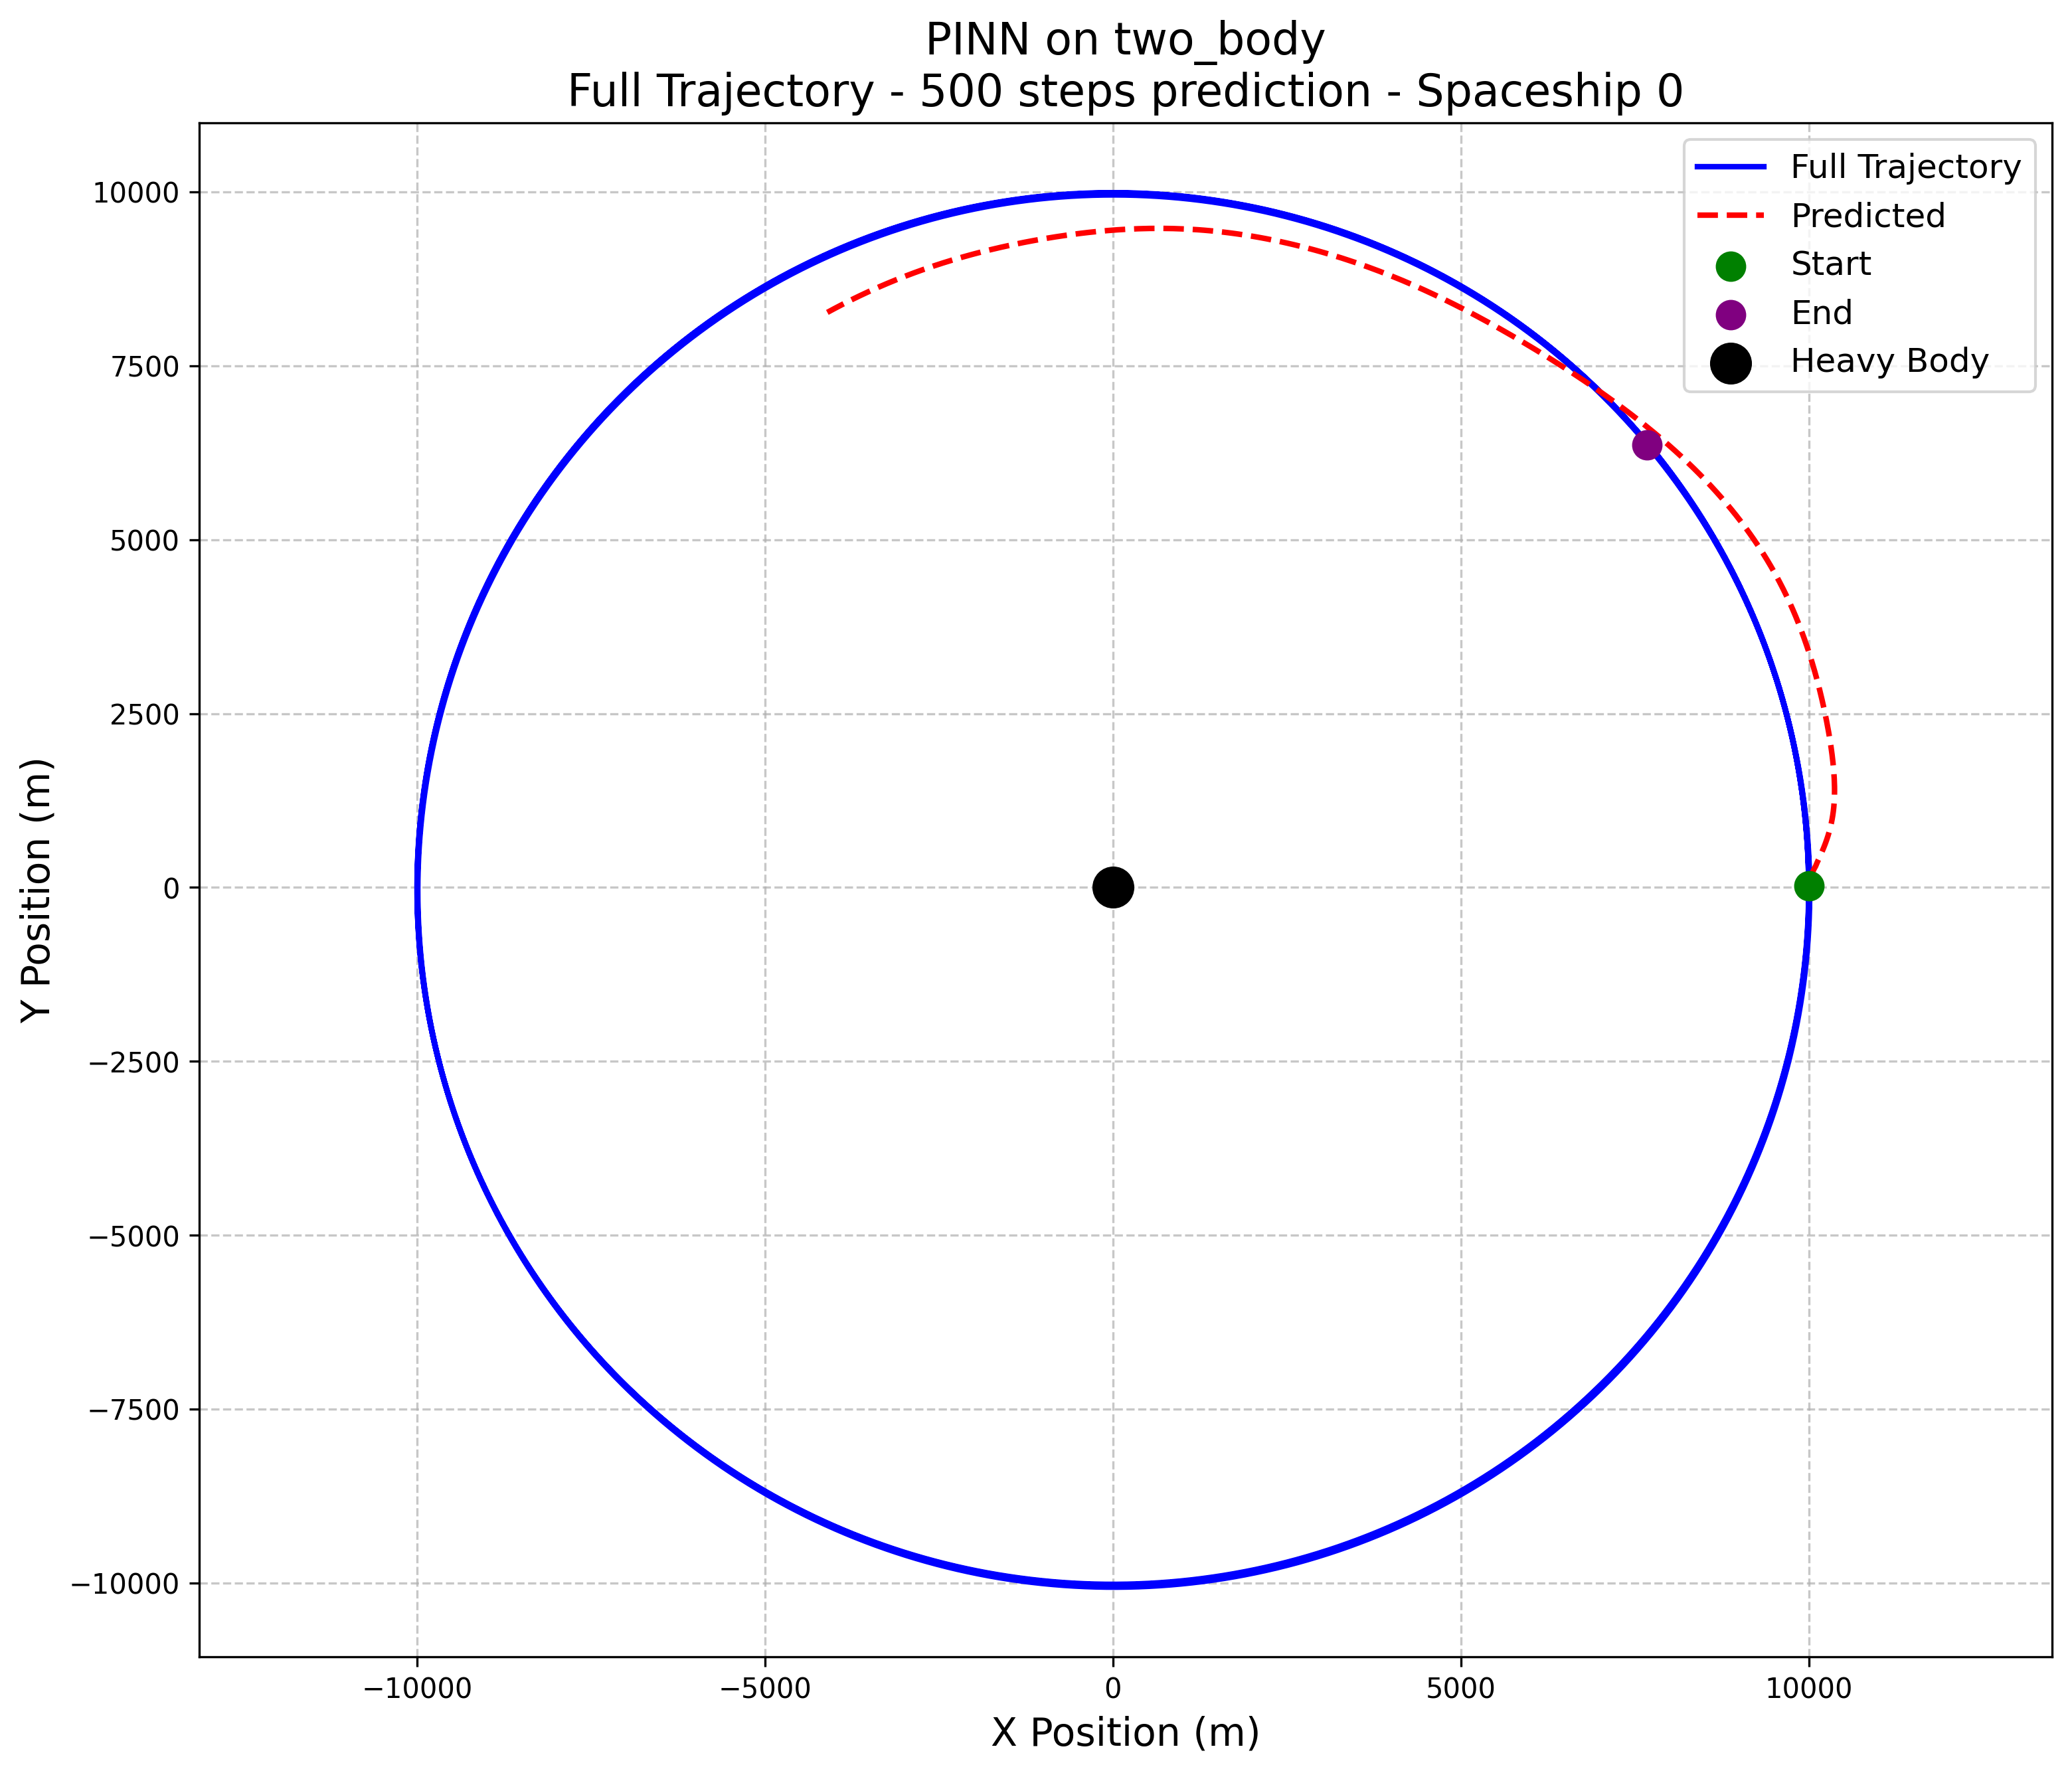
\includegraphics[width=0.27\textwidth]{../inference_results/val/PINN/two_body/500/full_trajectory_spaceship_0.png} &
      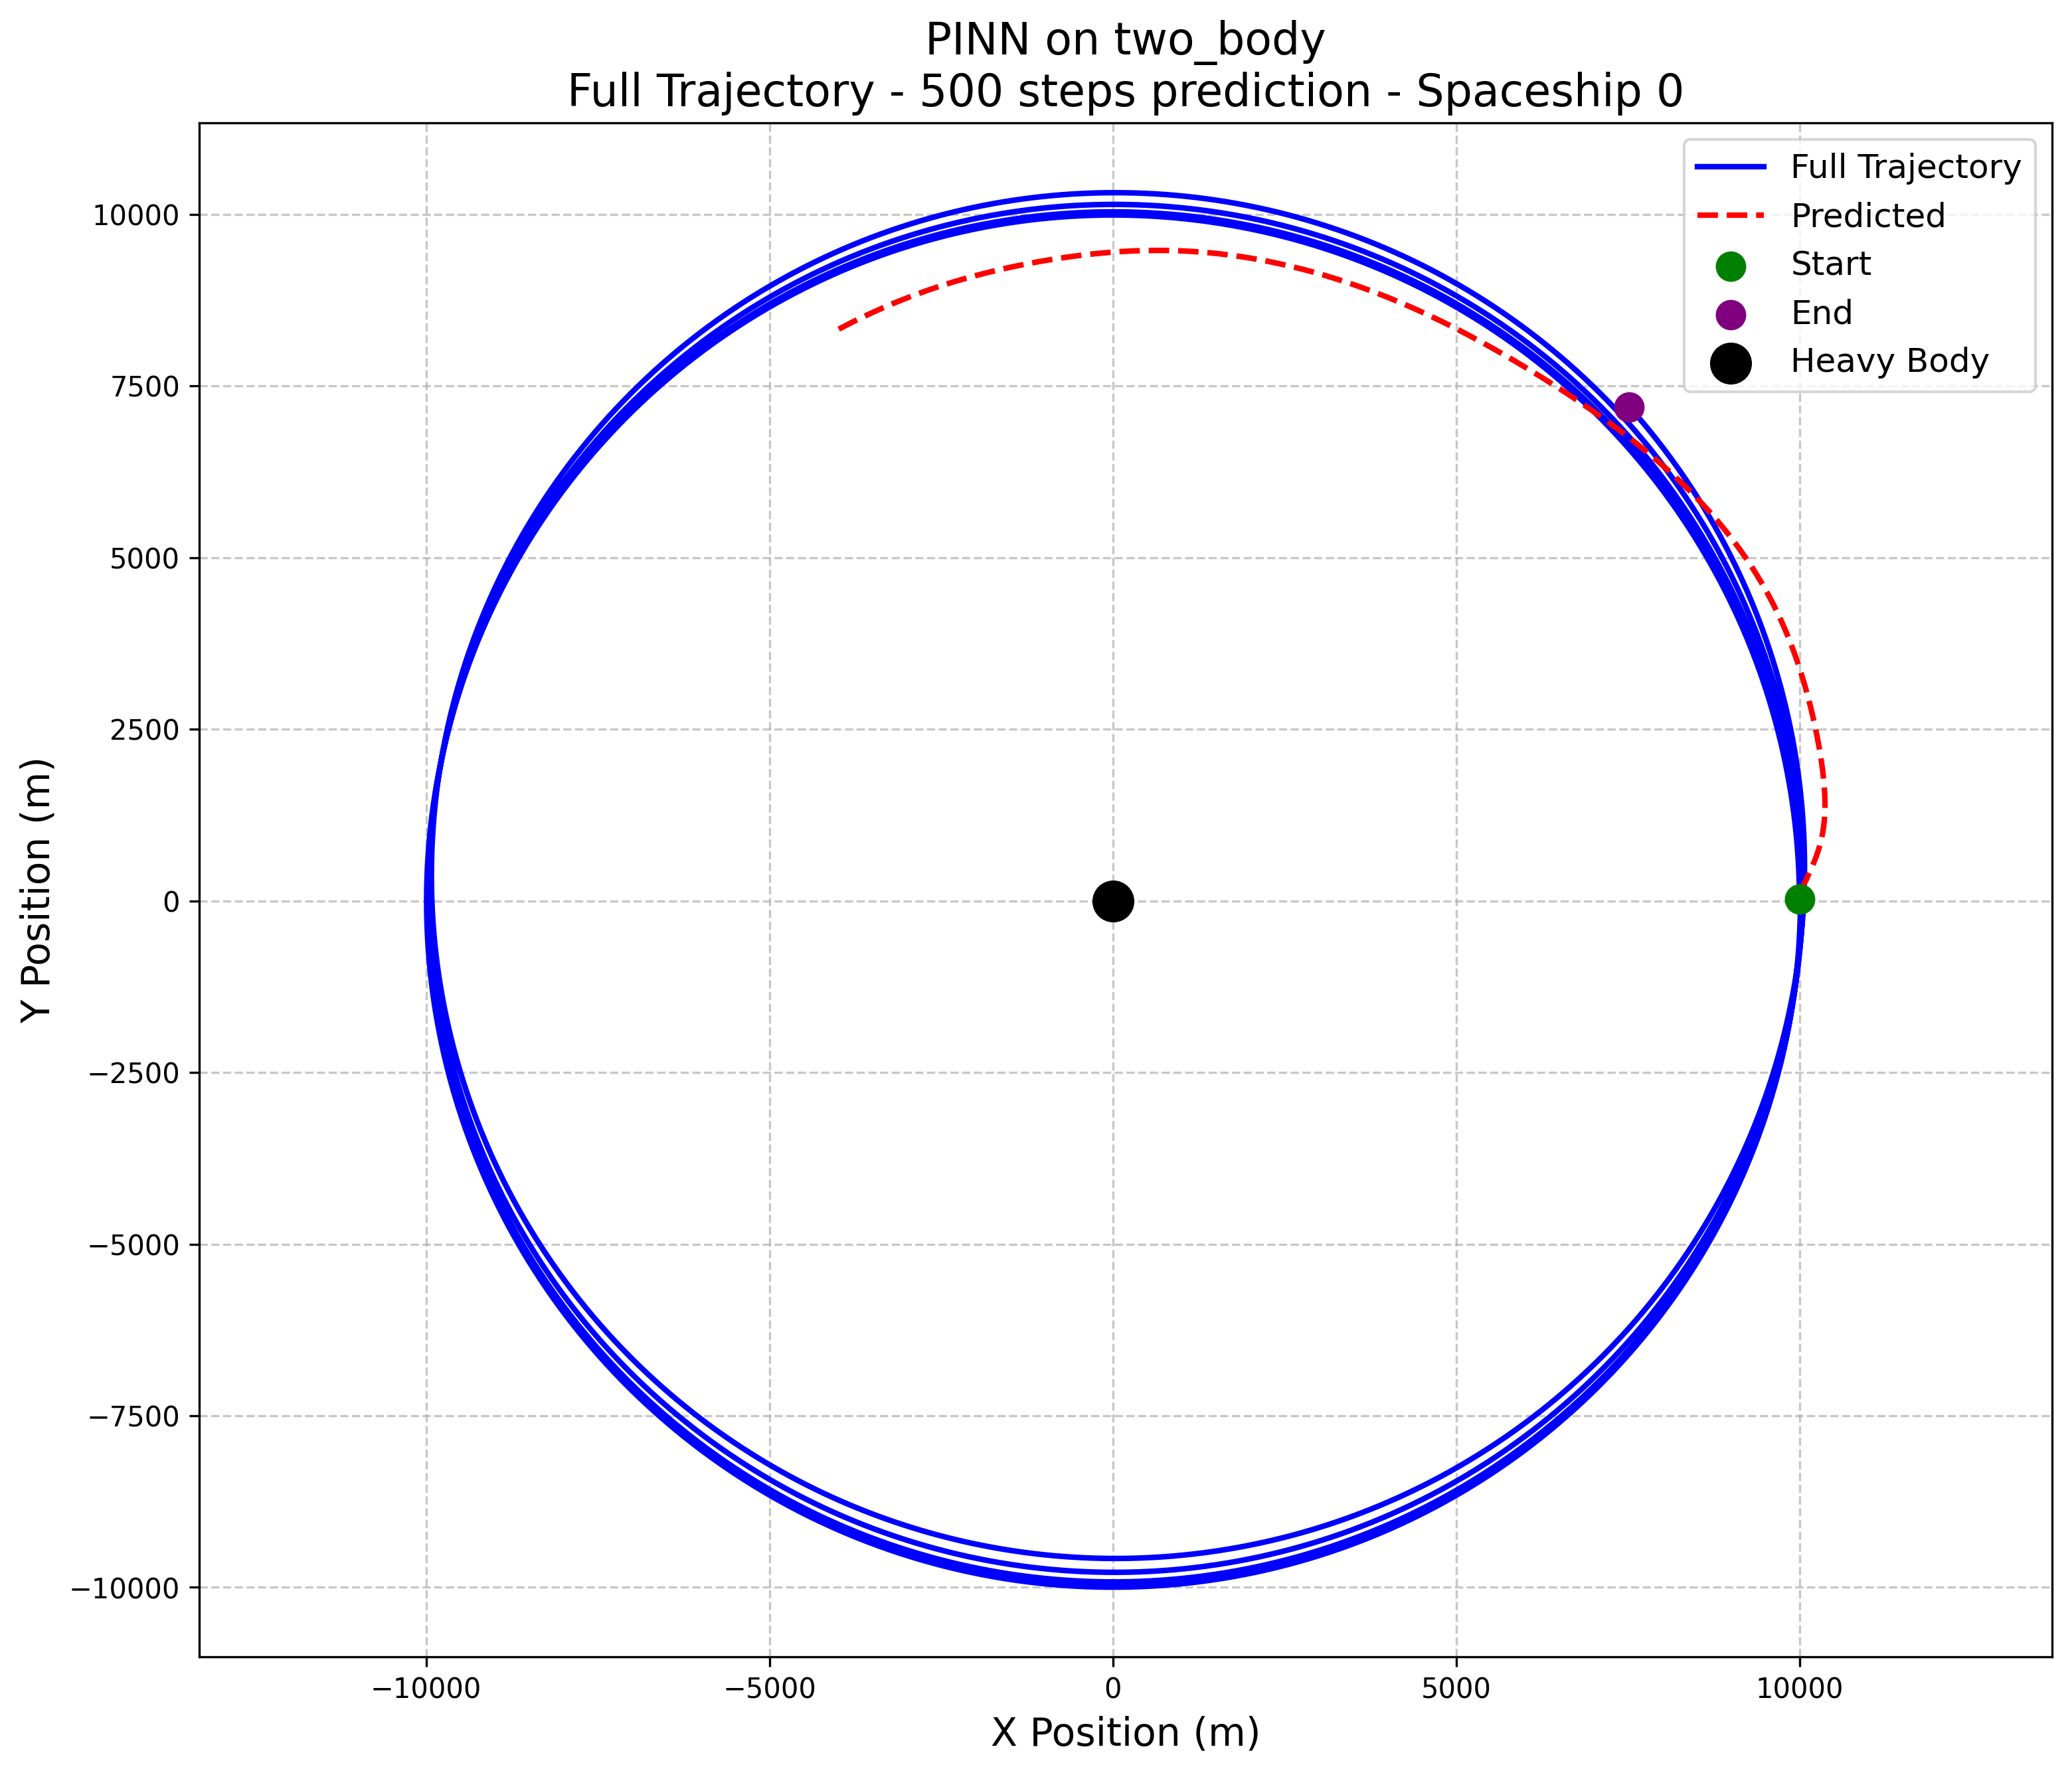
\includegraphics[width=0.27\textwidth]{../inference_results/test/PINN/two_body/500/full_trajectory_spaceship_0.png}
  \end{tabular}
\end{figure}

\section{Two-Body Problem with Increased Acceleration Trajectory Predictions}
\begin{figure}[H]
  \centering
  \caption{Two-Body Problem with Increased Acceleration: Model Predictions vs. Actual Trajectories}
  \label{fig:two_body_acc_predictions}
  \begin{tabular}{cccc}
      & Train & Validation & Test \\
      MLP &
      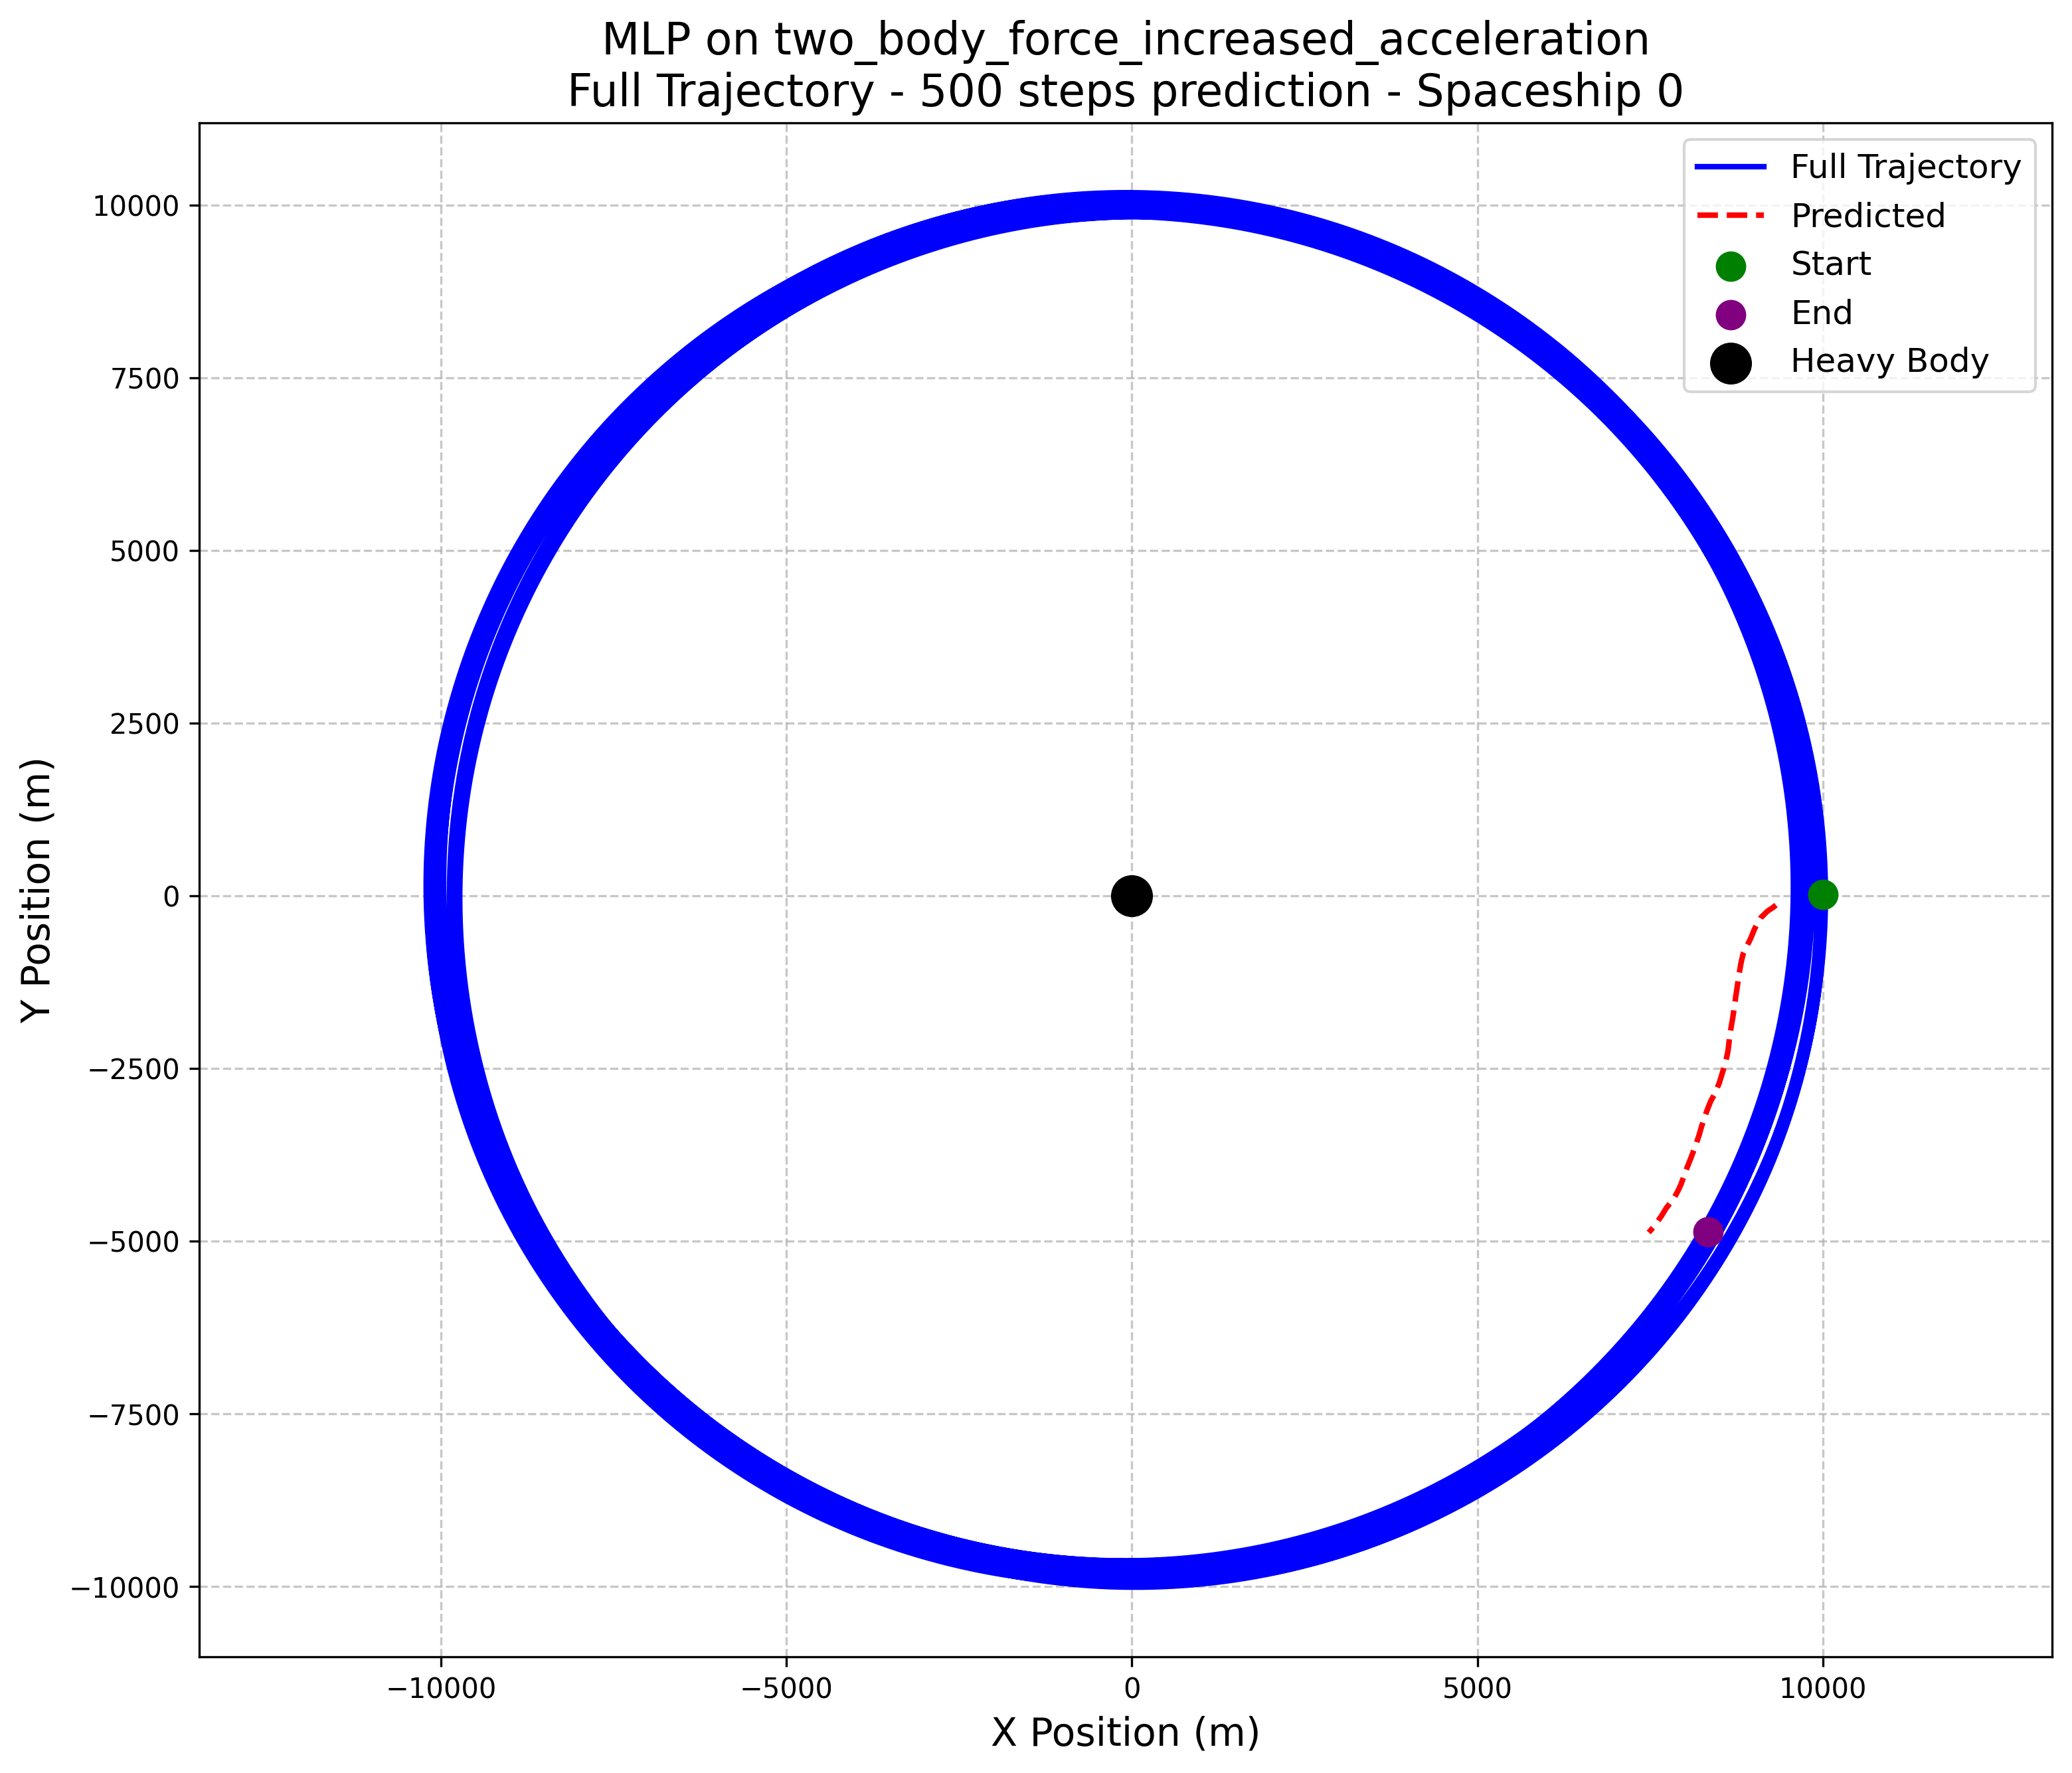
\includegraphics[width=0.27\textwidth]{../inference_results/train/MLP/two_body_force_increased_acceleration/500/full_trajectory_spaceship_0.png} &
      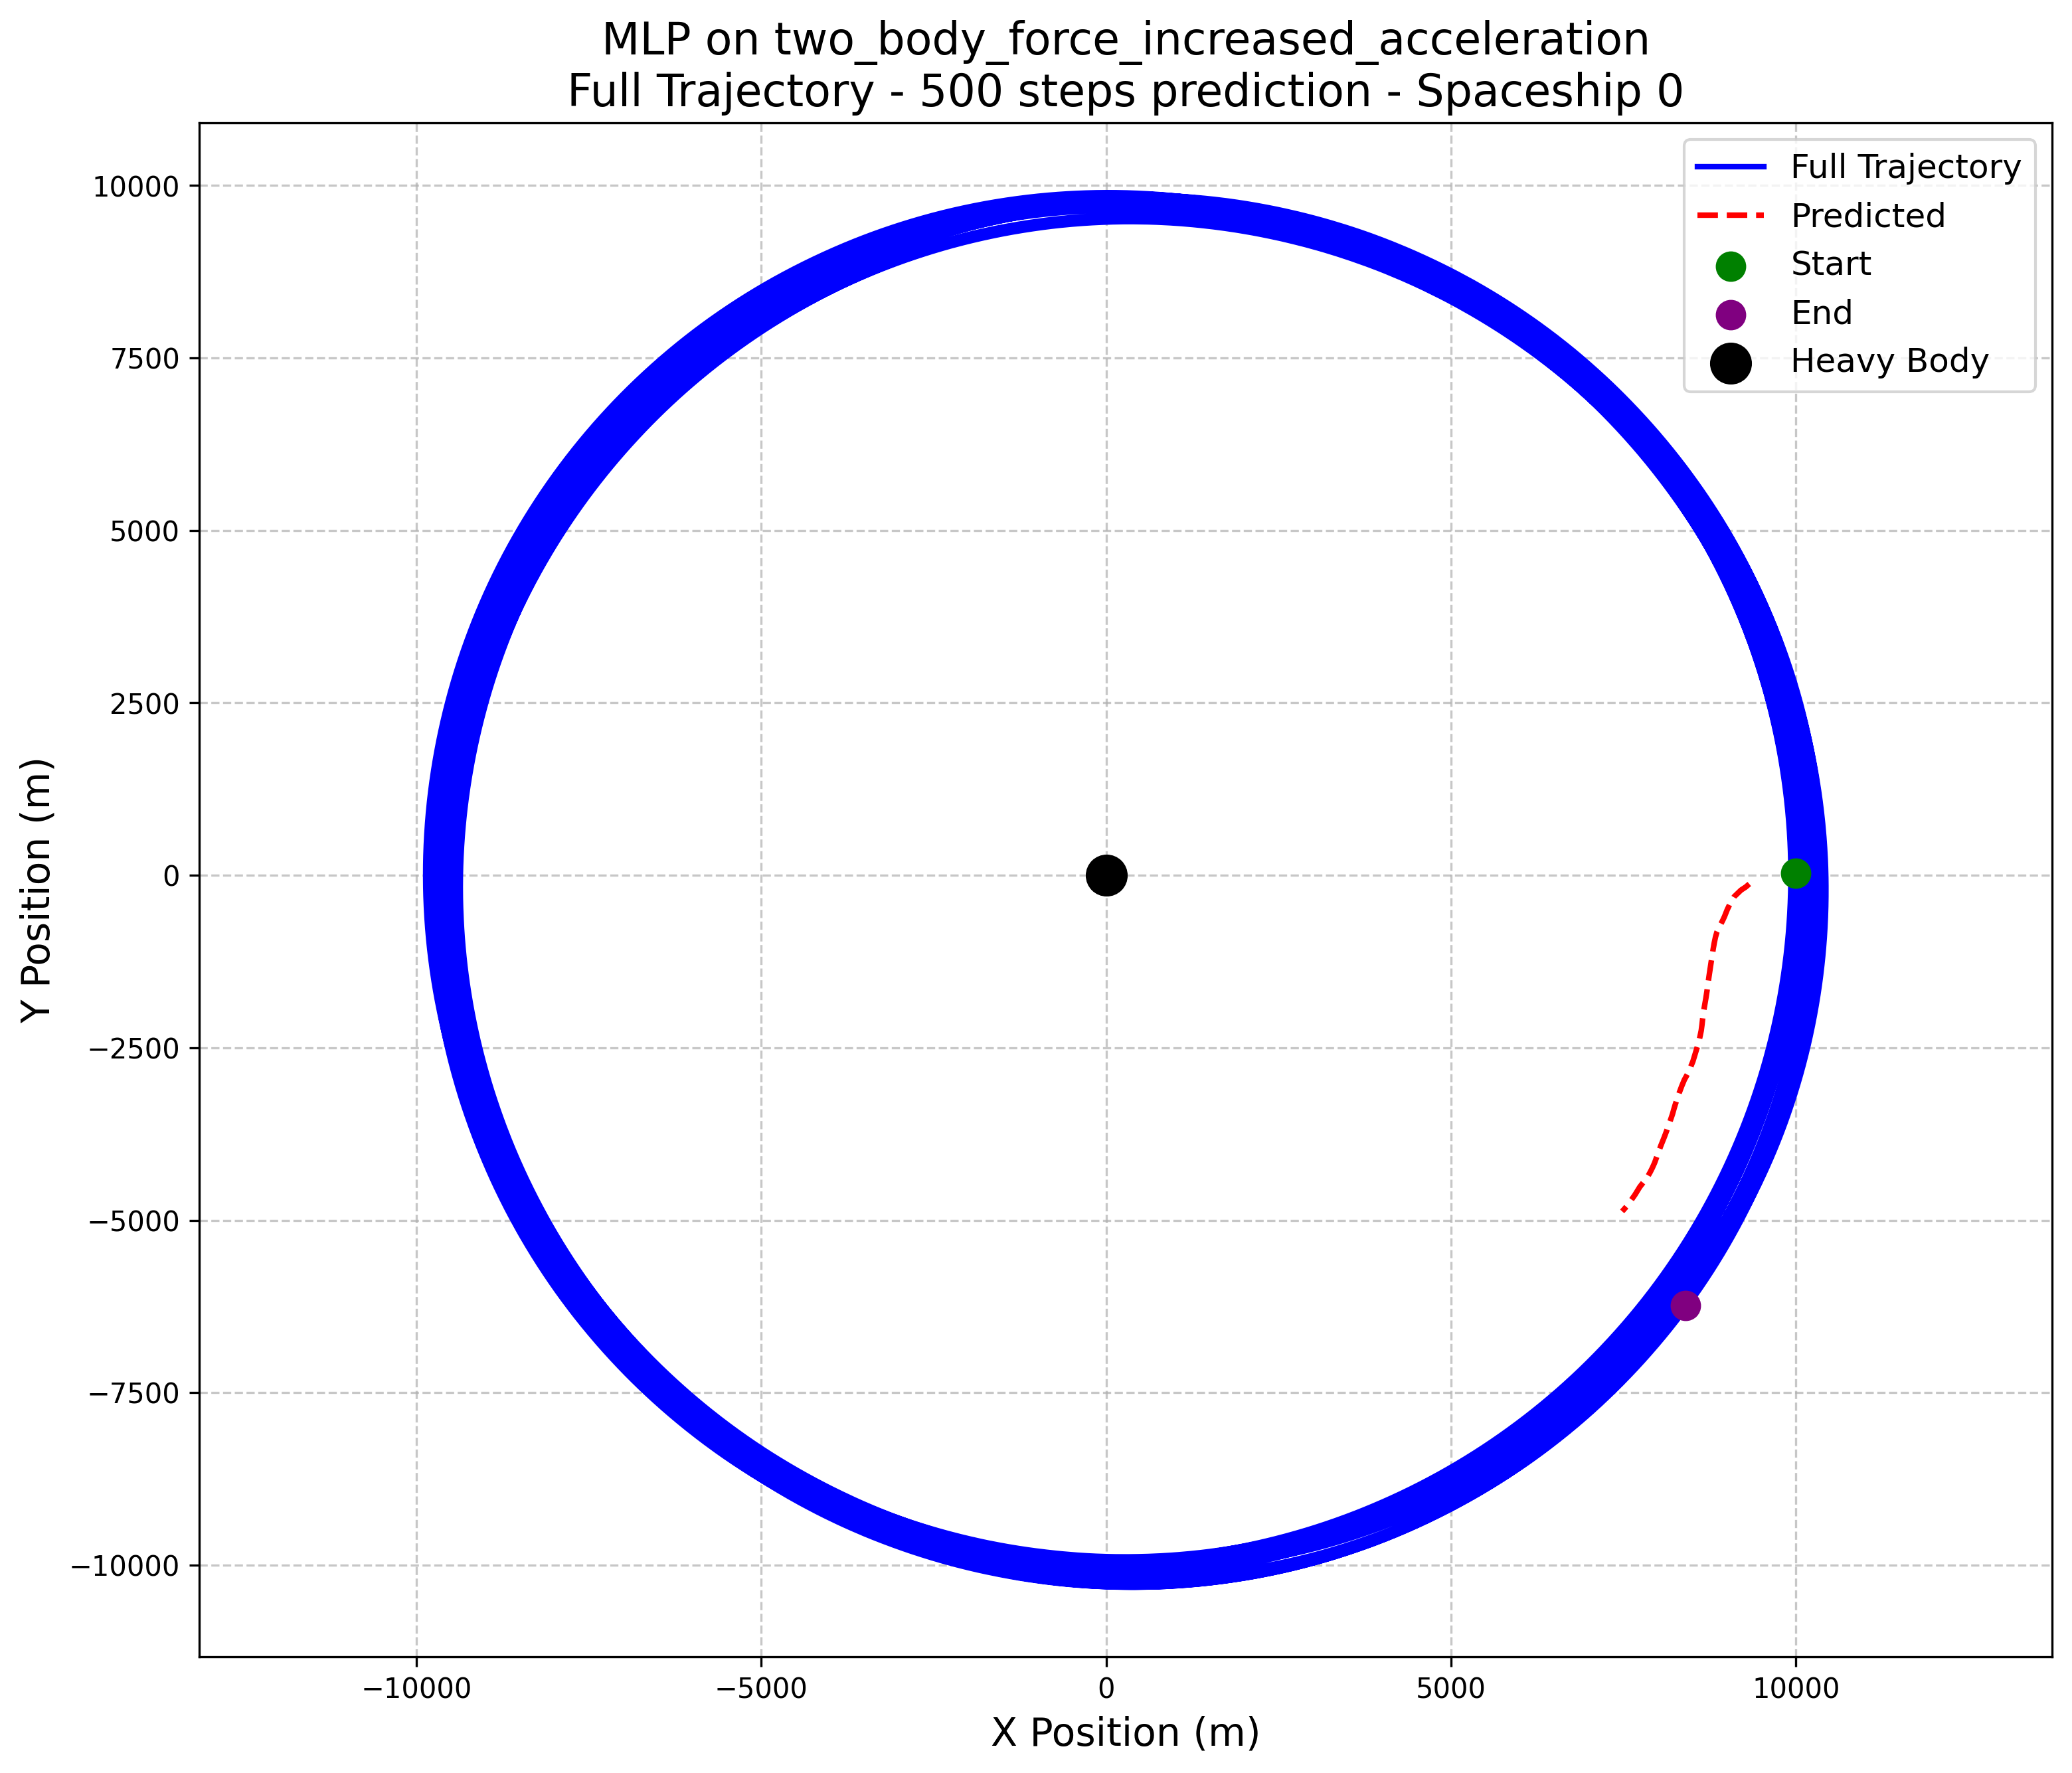
\includegraphics[width=0.27\textwidth]{../inference_results/val/MLP/two_body_force_increased_acceleration/500/full_trajectory_spaceship_0.png} &
      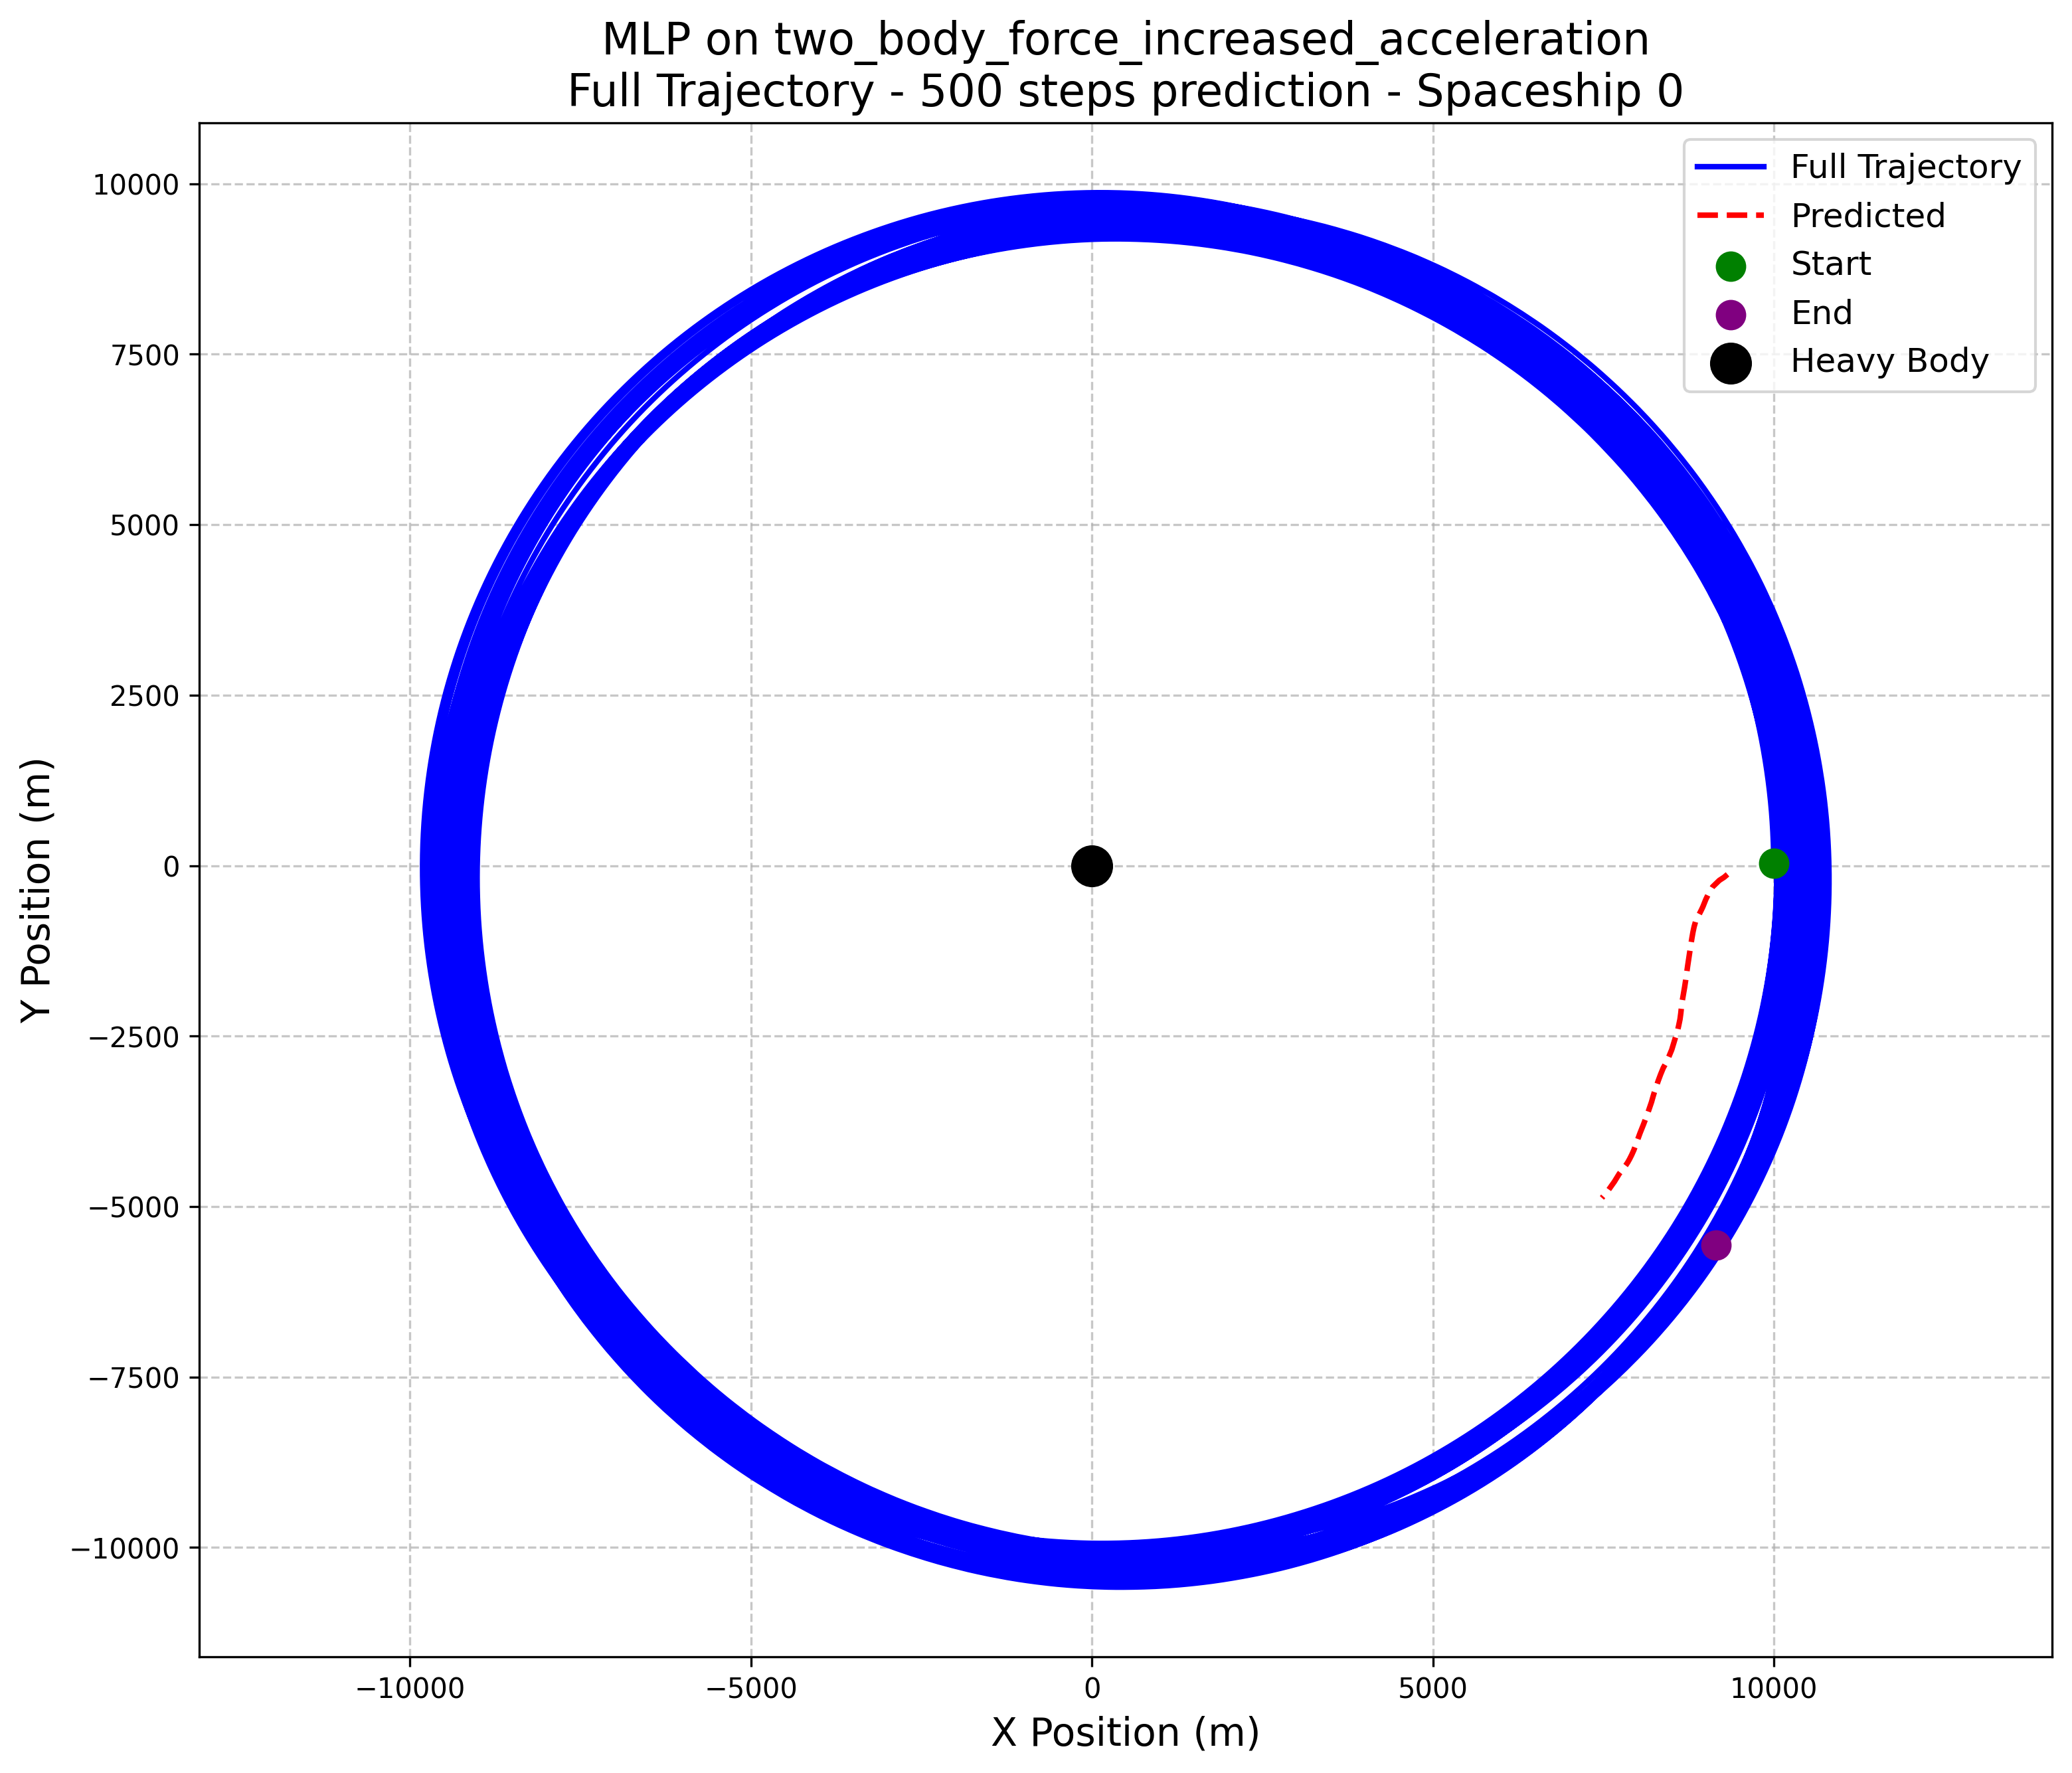
\includegraphics[width=0.27\textwidth]{../inference_results/test/MLP/two_body_force_increased_acceleration/500/full_trajectory_spaceship_0.png} \\
      LSTM &
      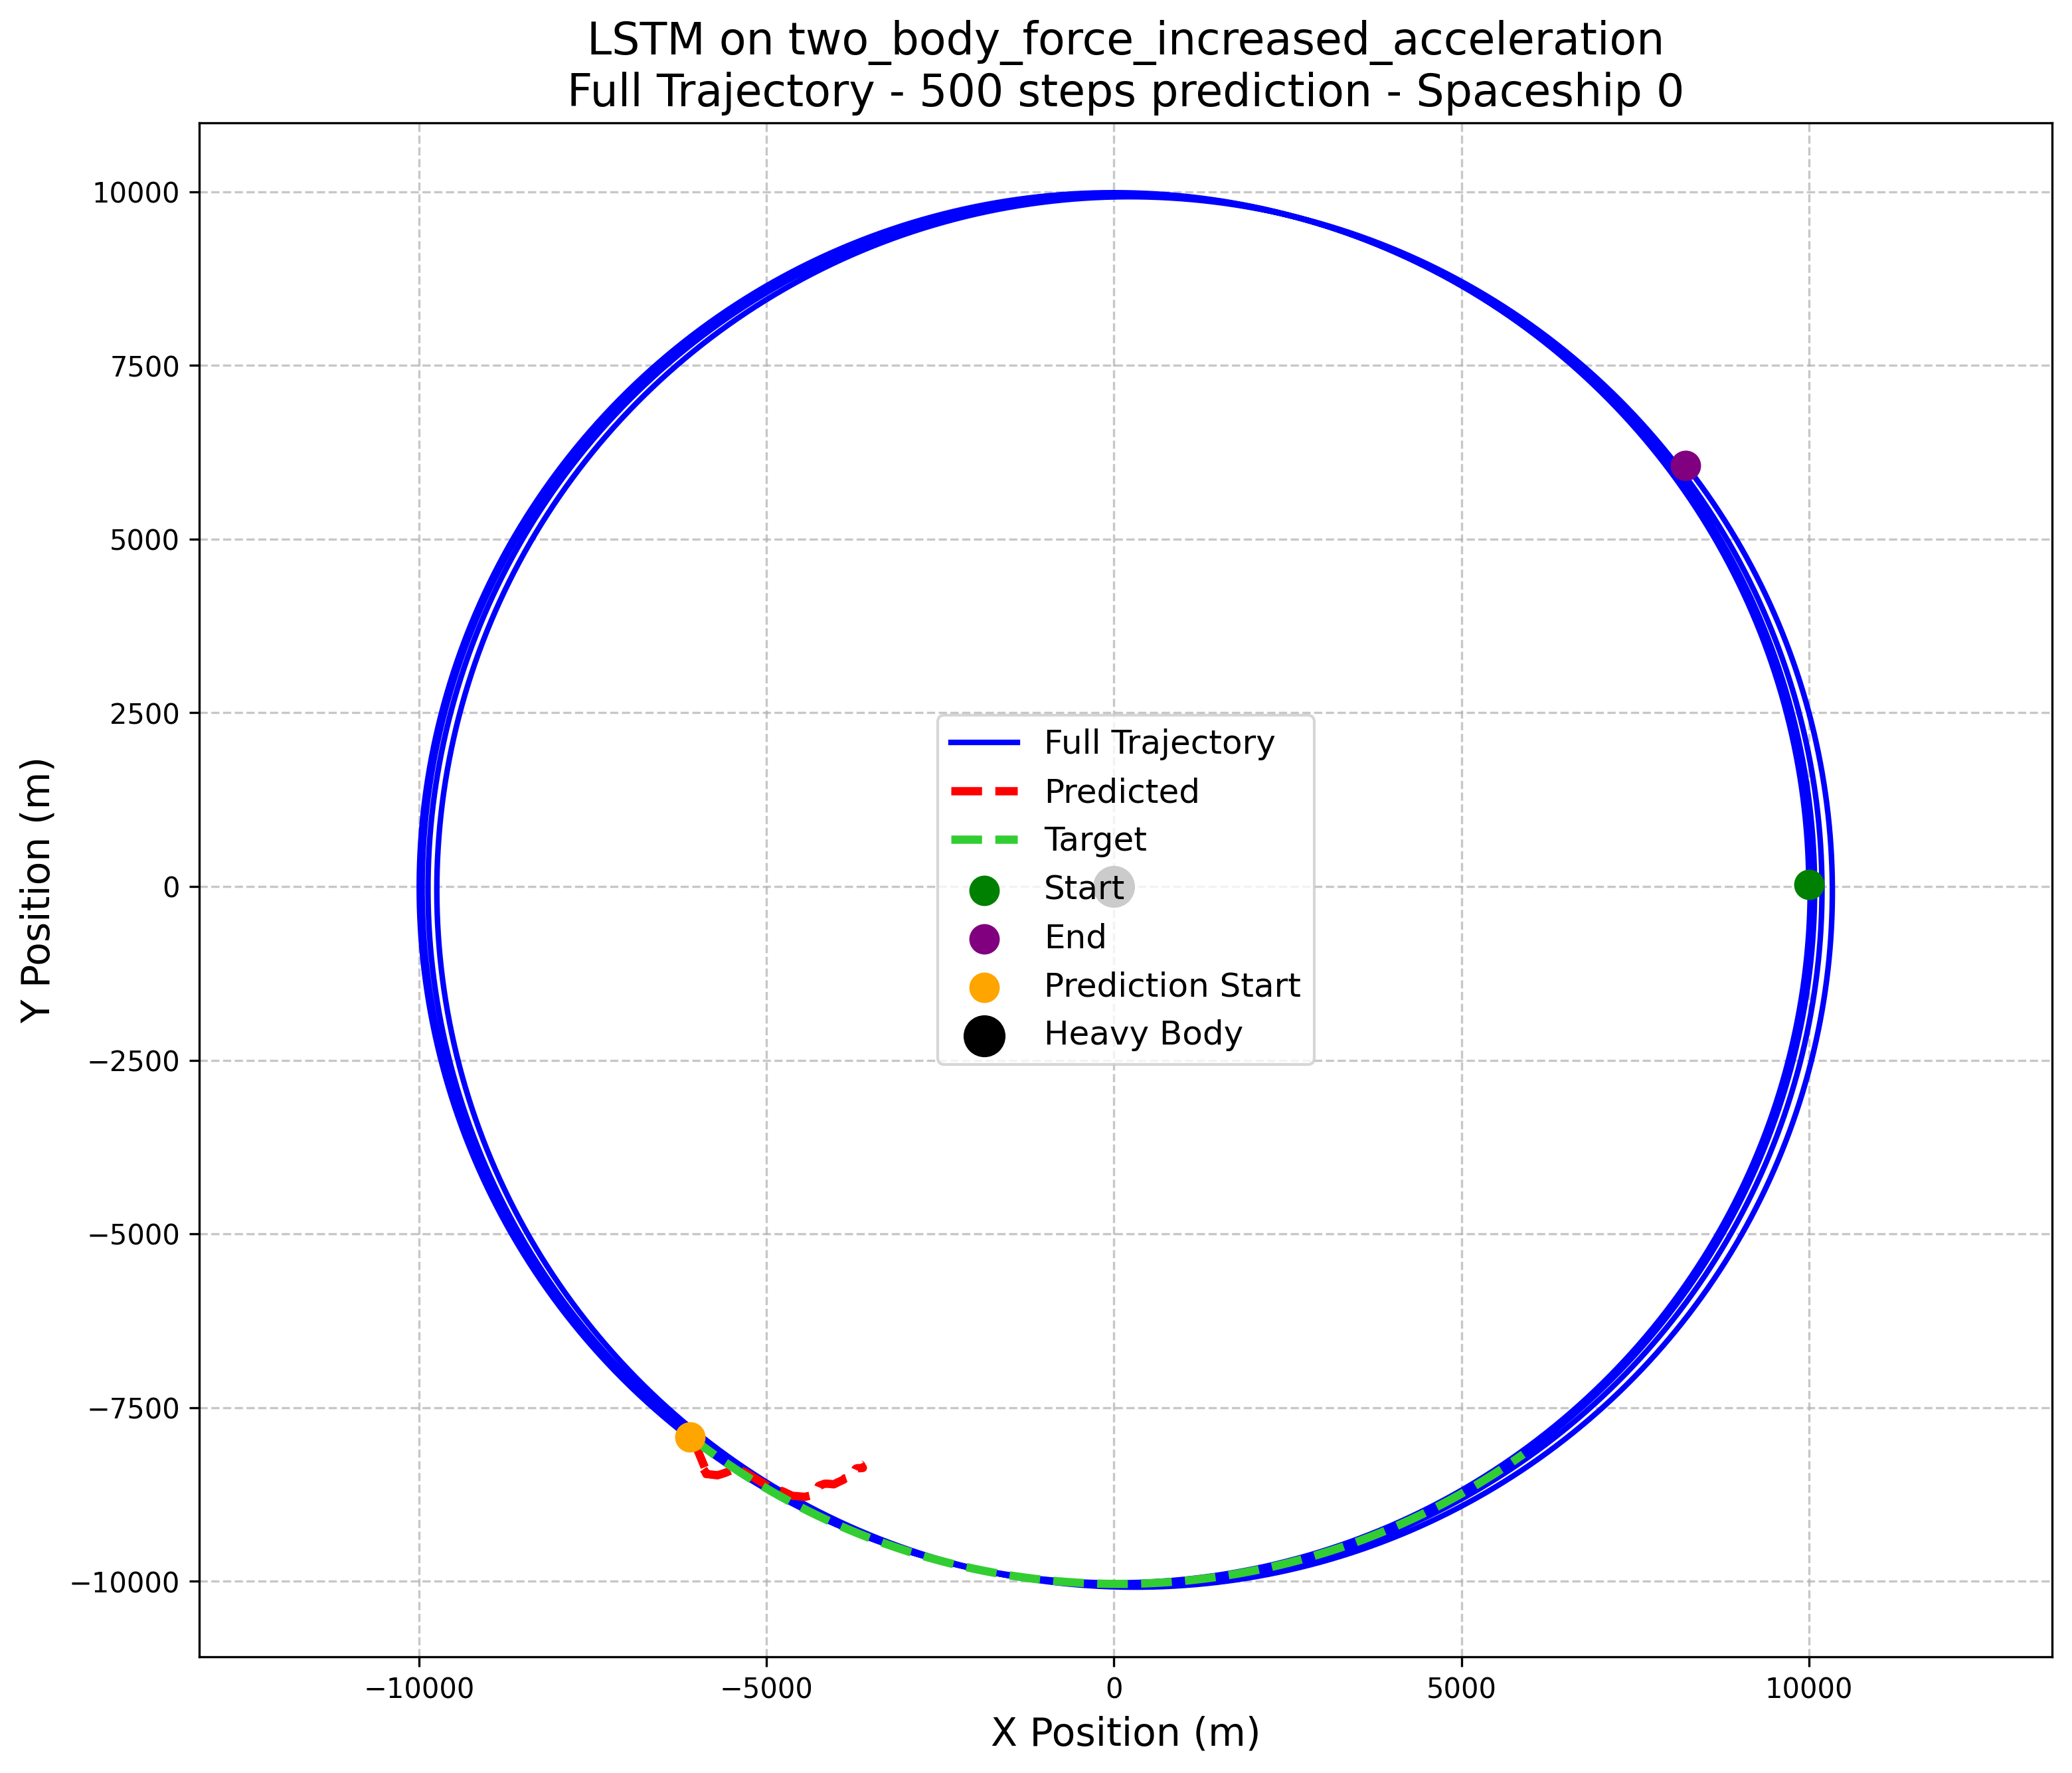
\includegraphics[width=0.27\textwidth]{../inference_results/train/LSTM/two_body_force_increased_acceleration/500/full_trajectory_spaceship_0.png} &
      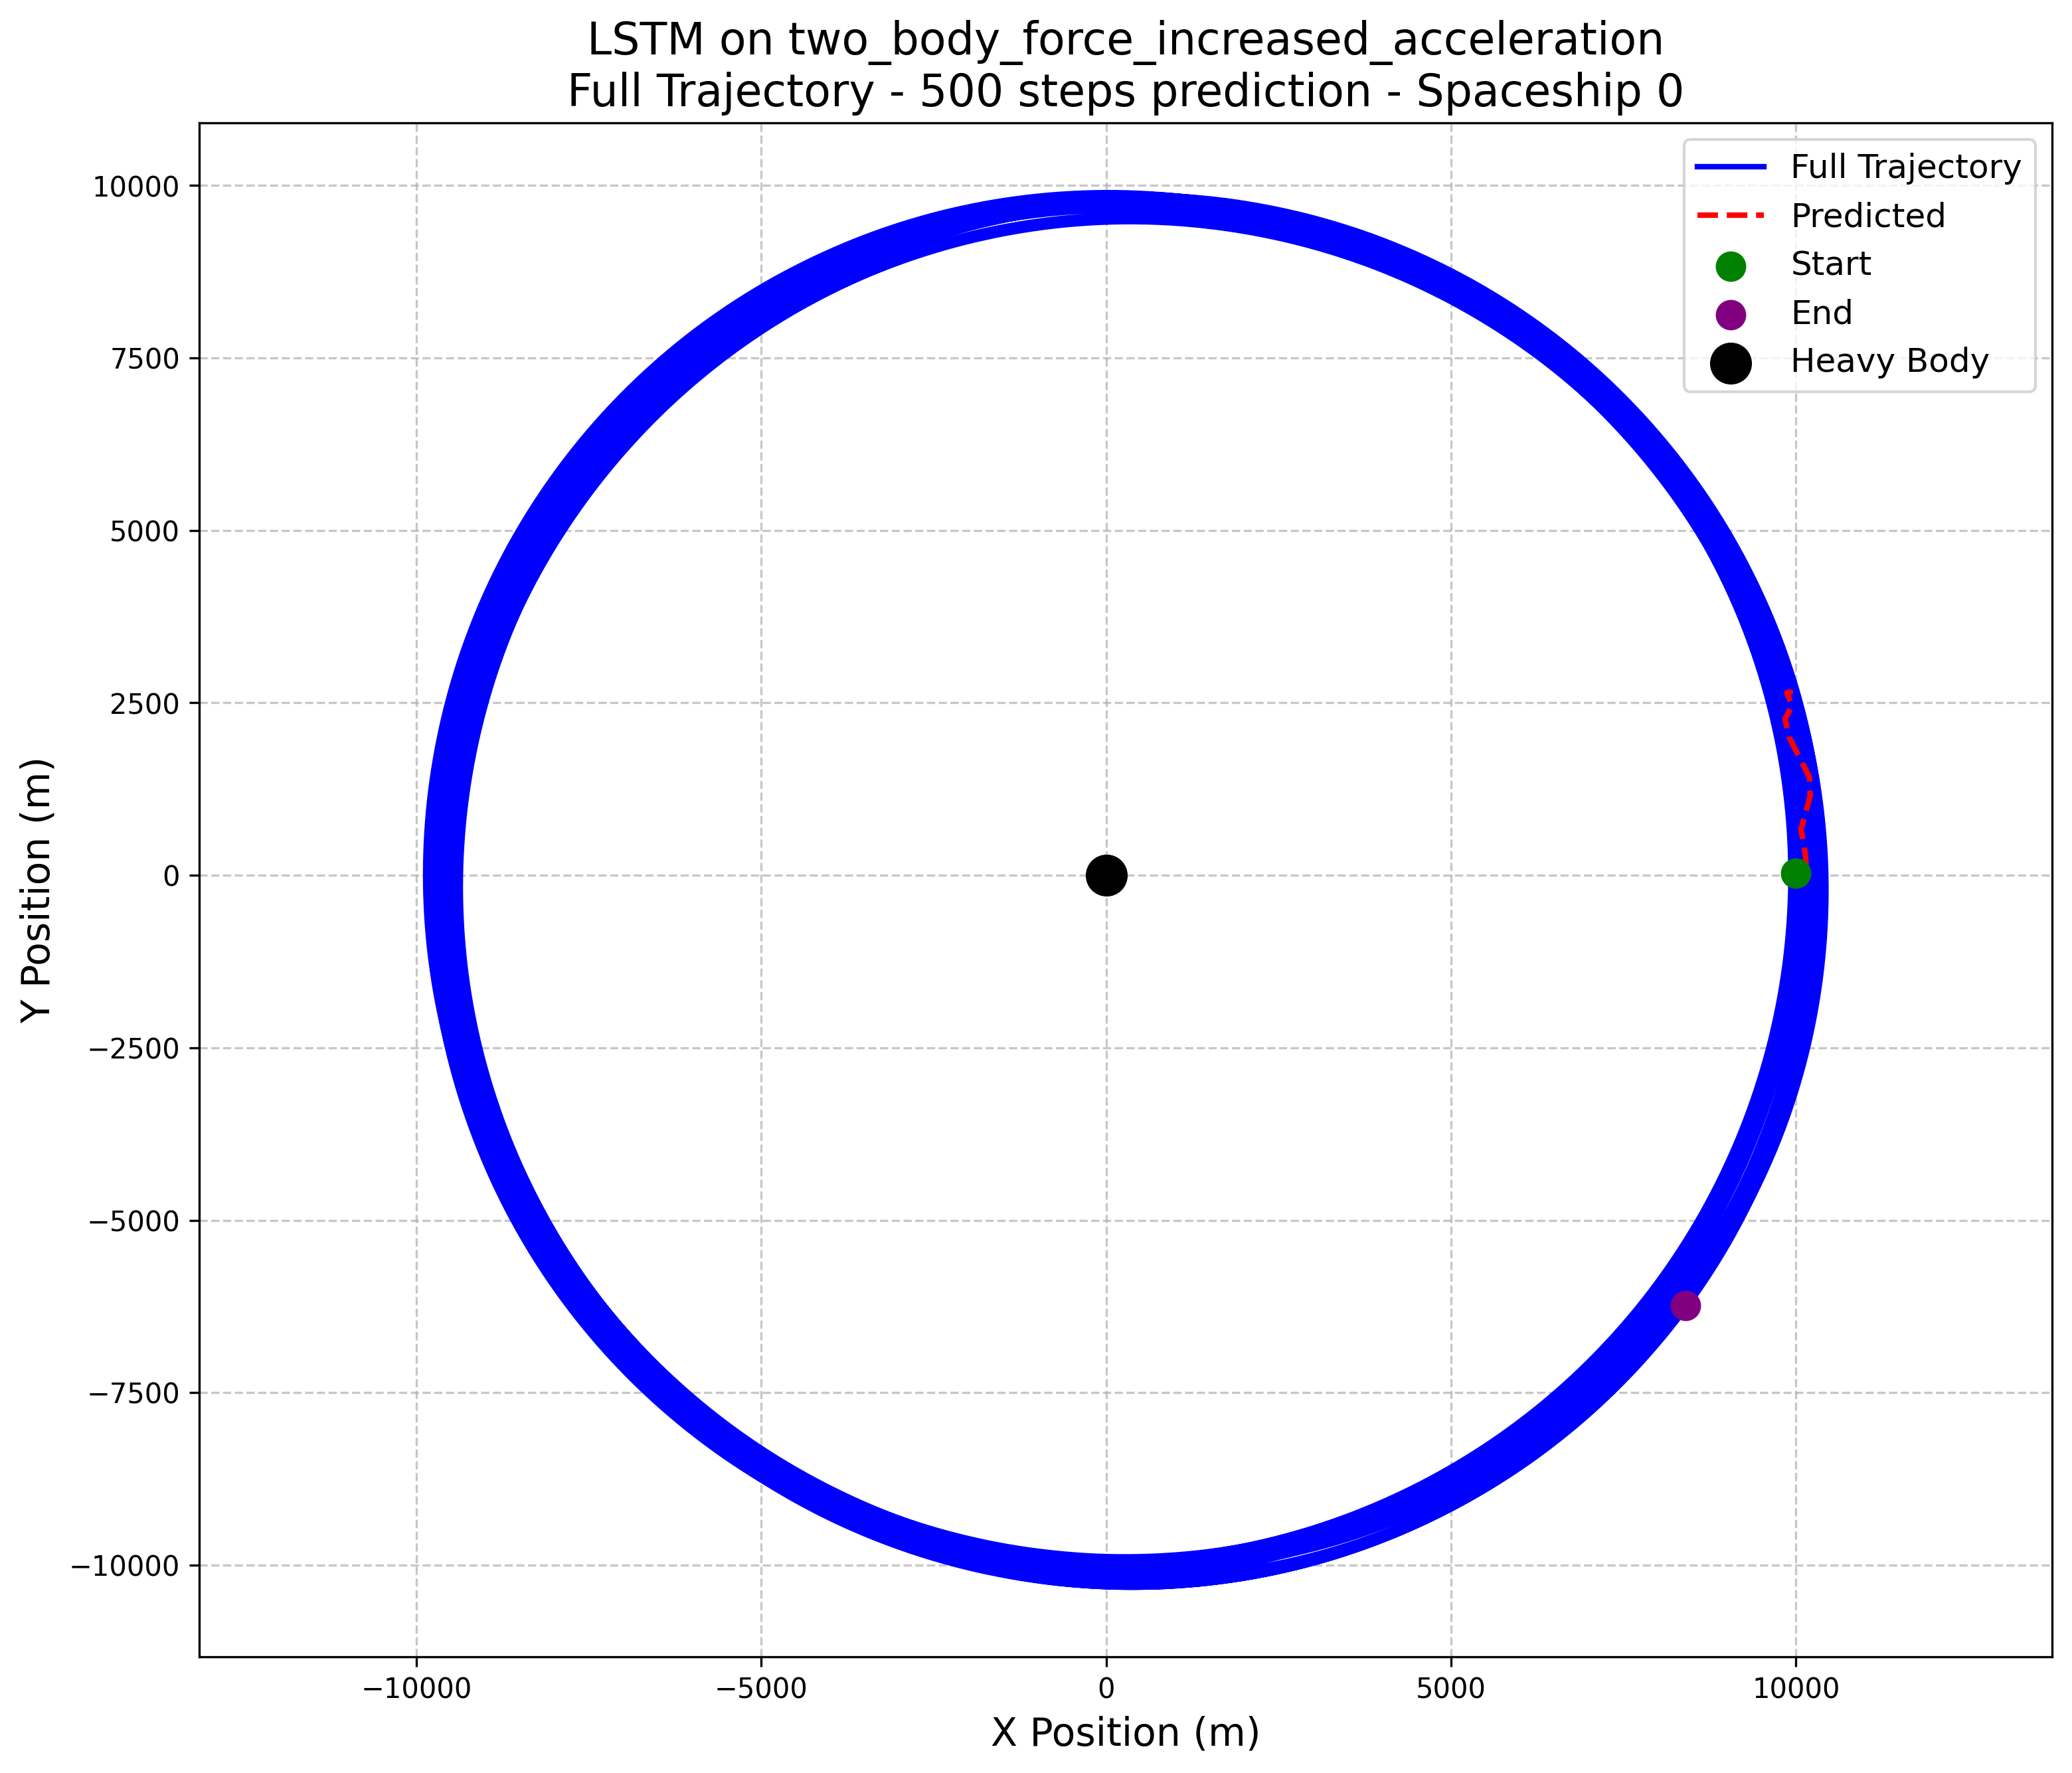
\includegraphics[width=0.27\textwidth]{../inference_results/val/LSTM/two_body_force_increased_acceleration/500/full_trajectory_spaceship_0.png} &
      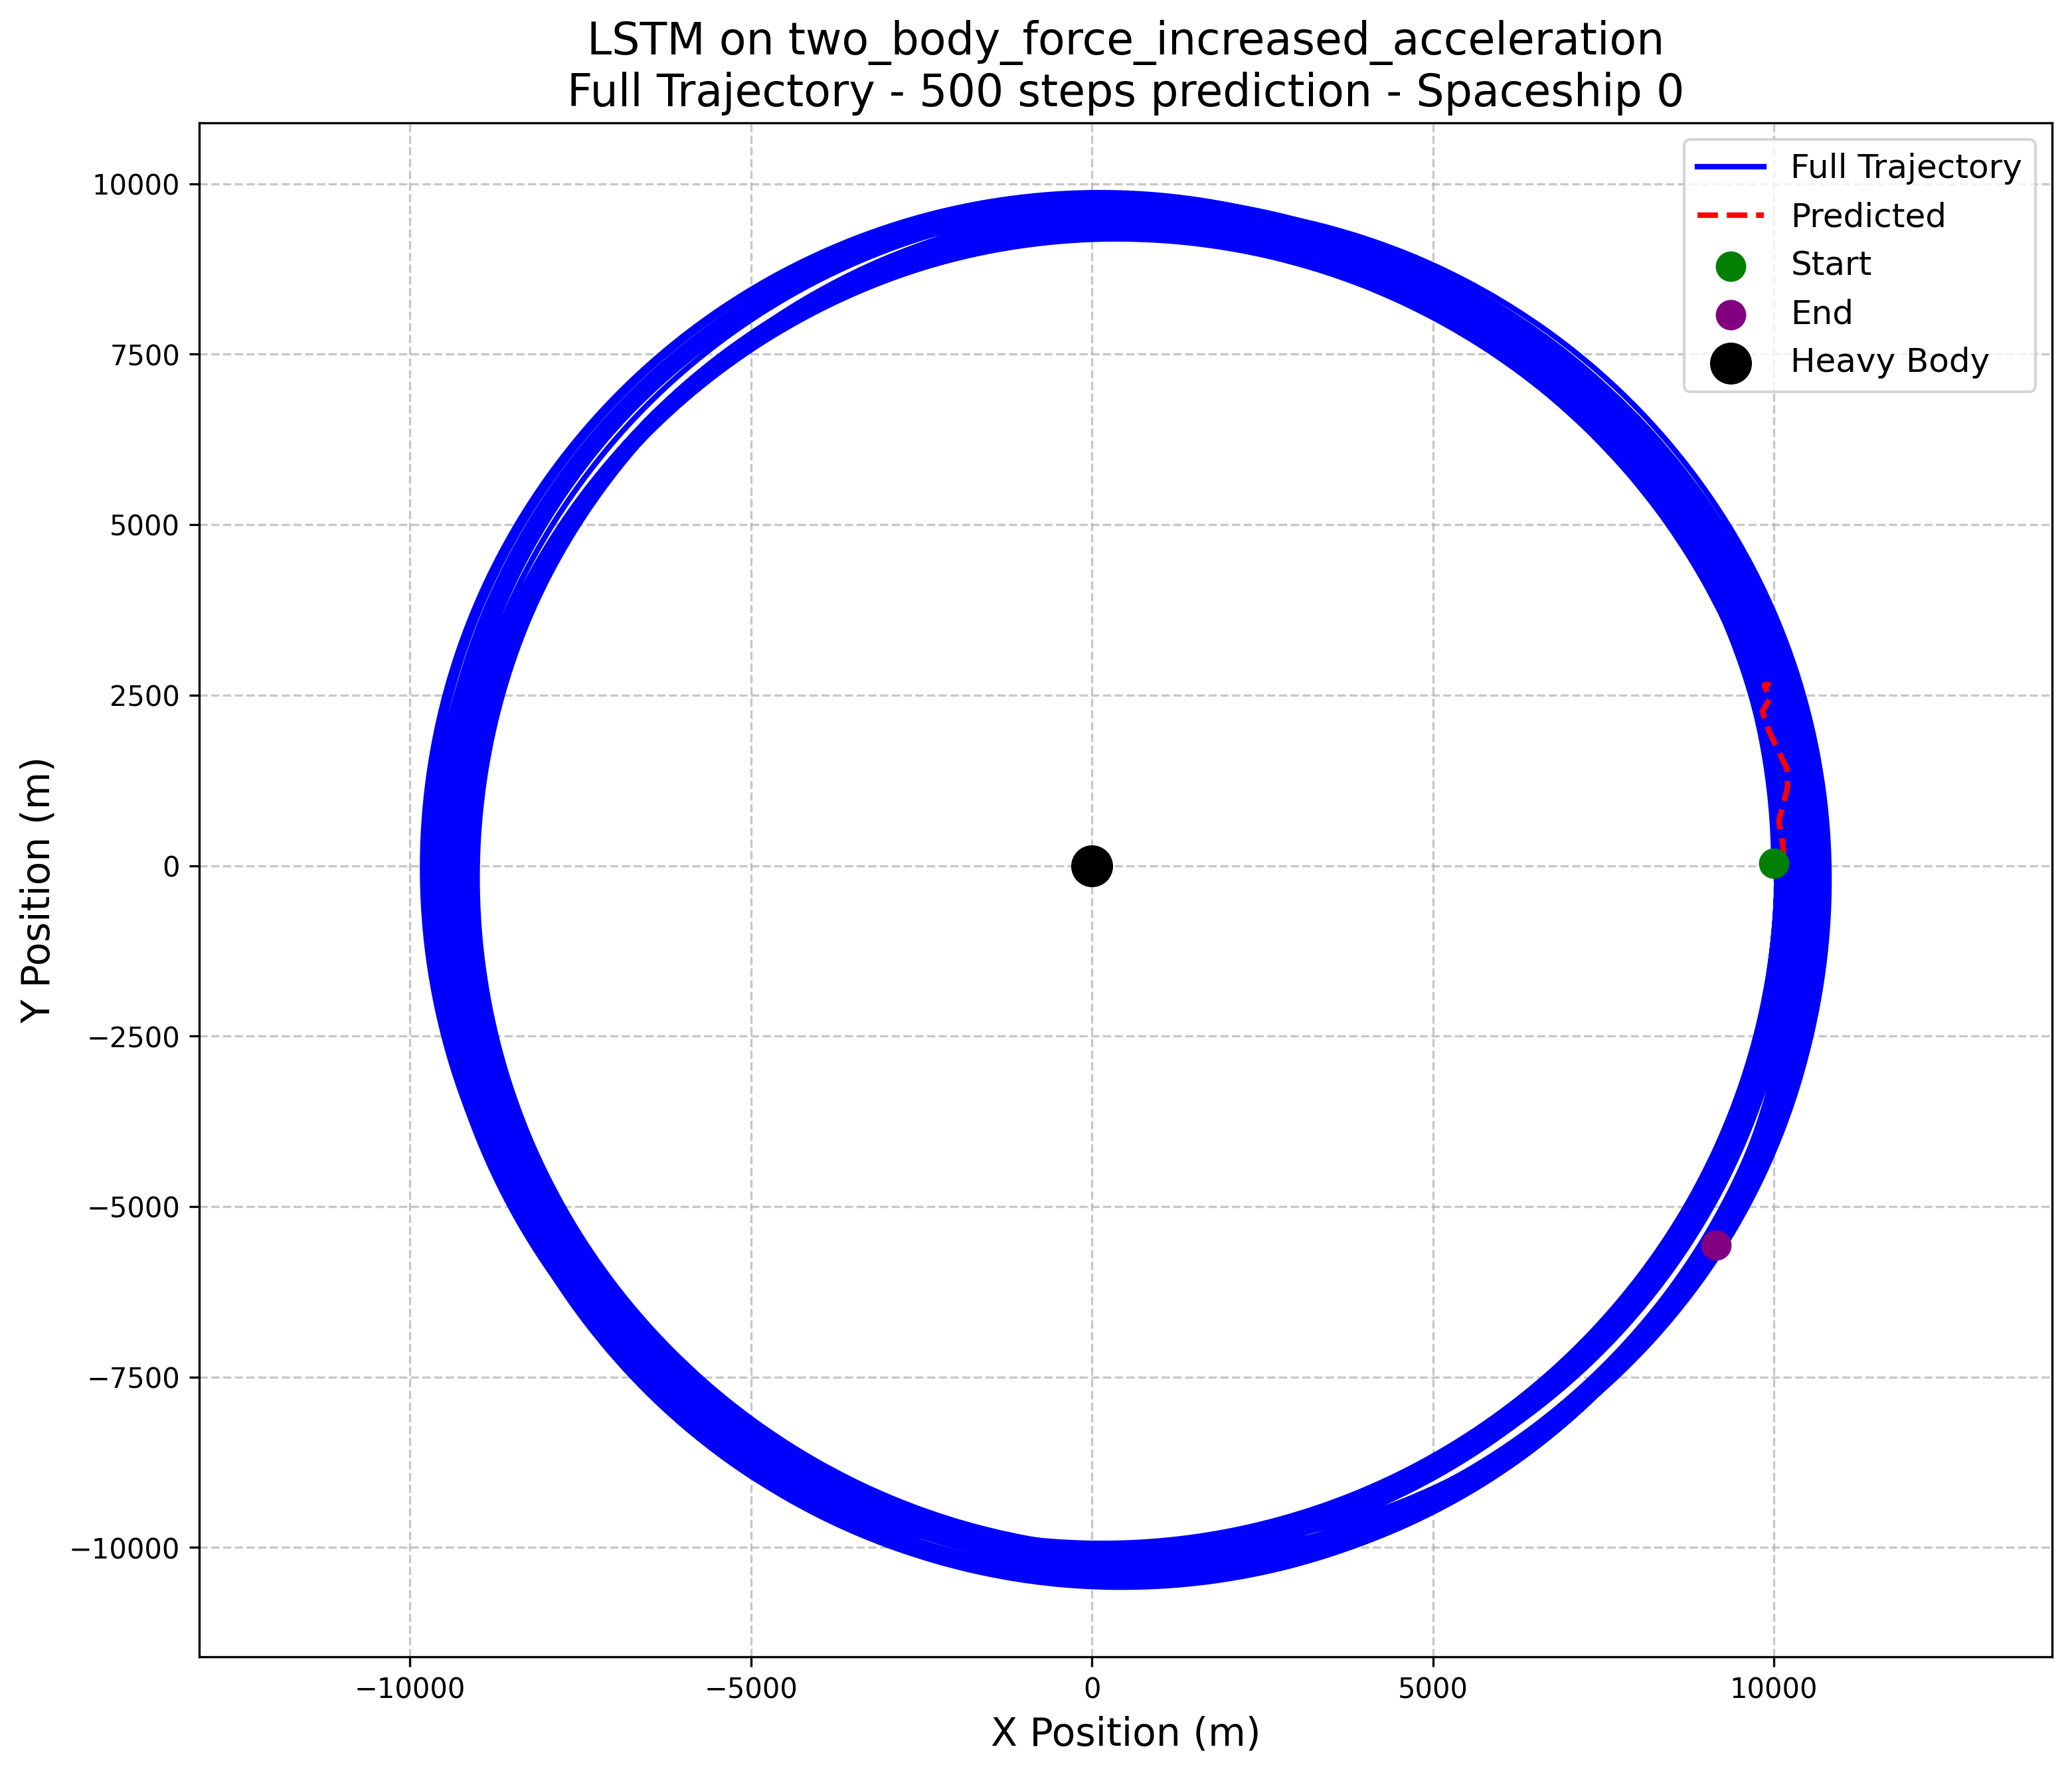
\includegraphics[width=0.27\textwidth]{../inference_results/test/LSTM/two_body_force_increased_acceleration/500/full_trajectory_spaceship_0.png} \\
      PINN &
      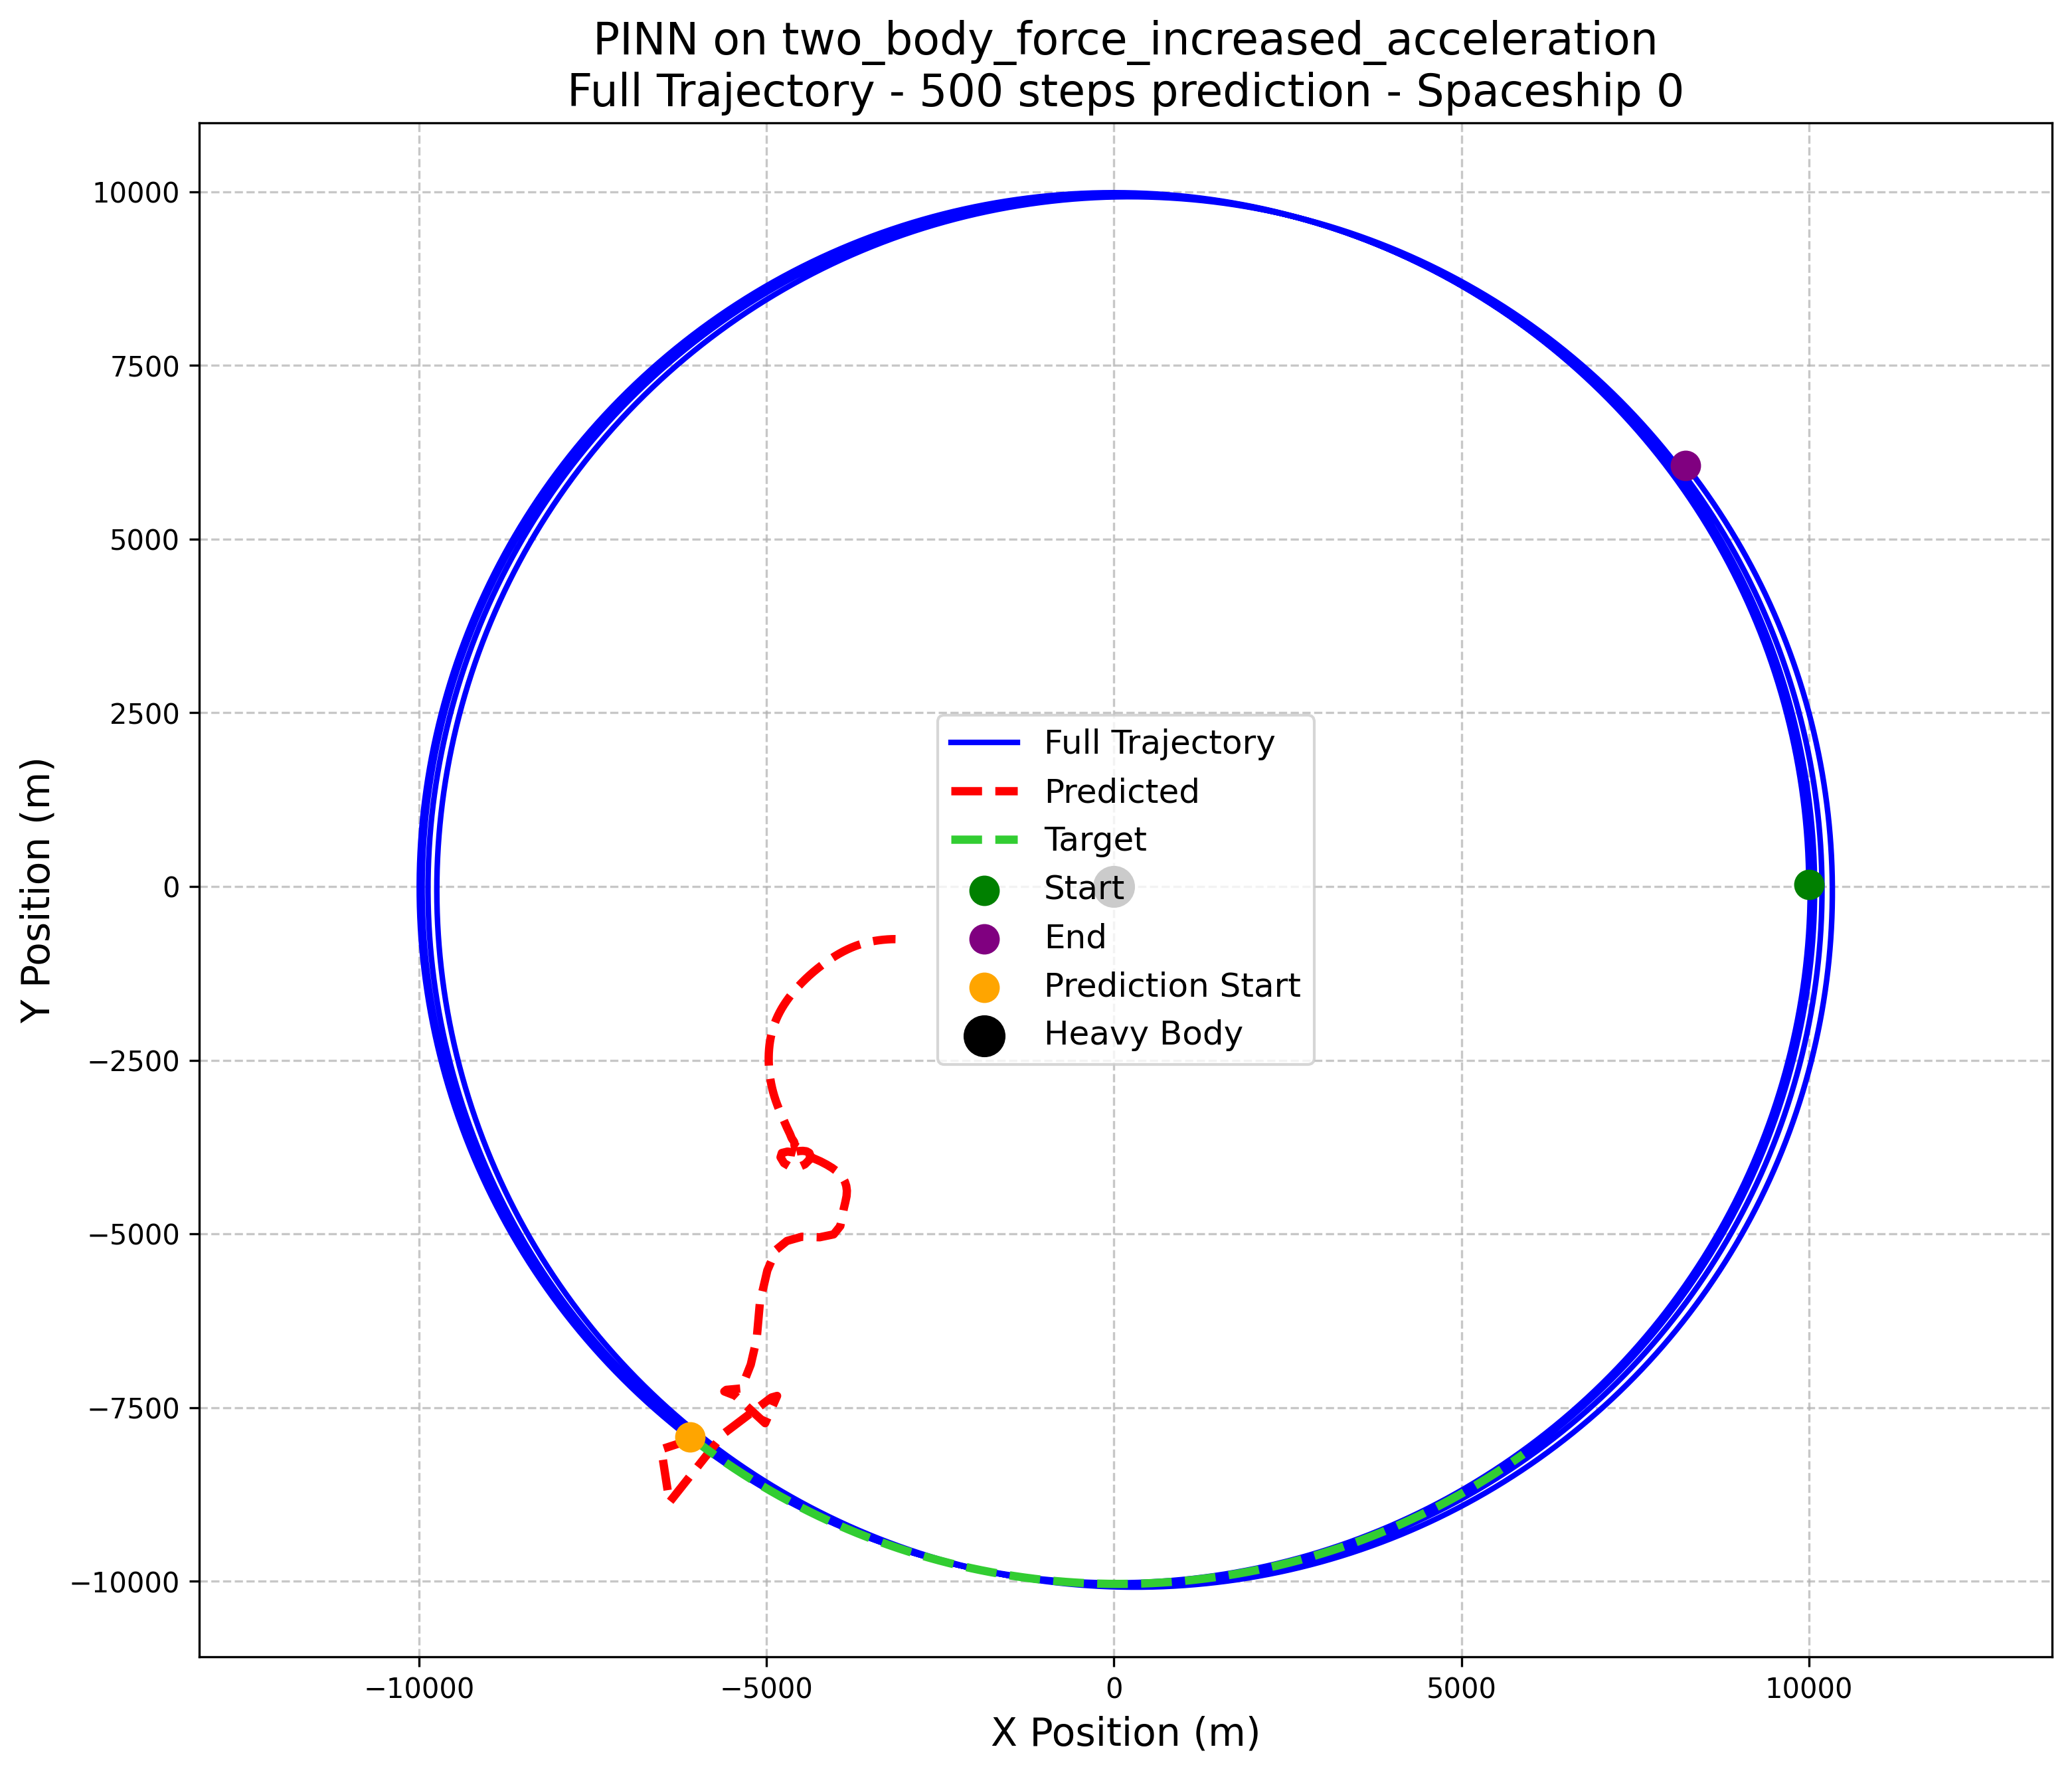
\includegraphics[width=0.27\textwidth]{../inference_results/train/PINN/two_body_force_increased_acceleration/500/full_trajectory_spaceship_0.png} &
      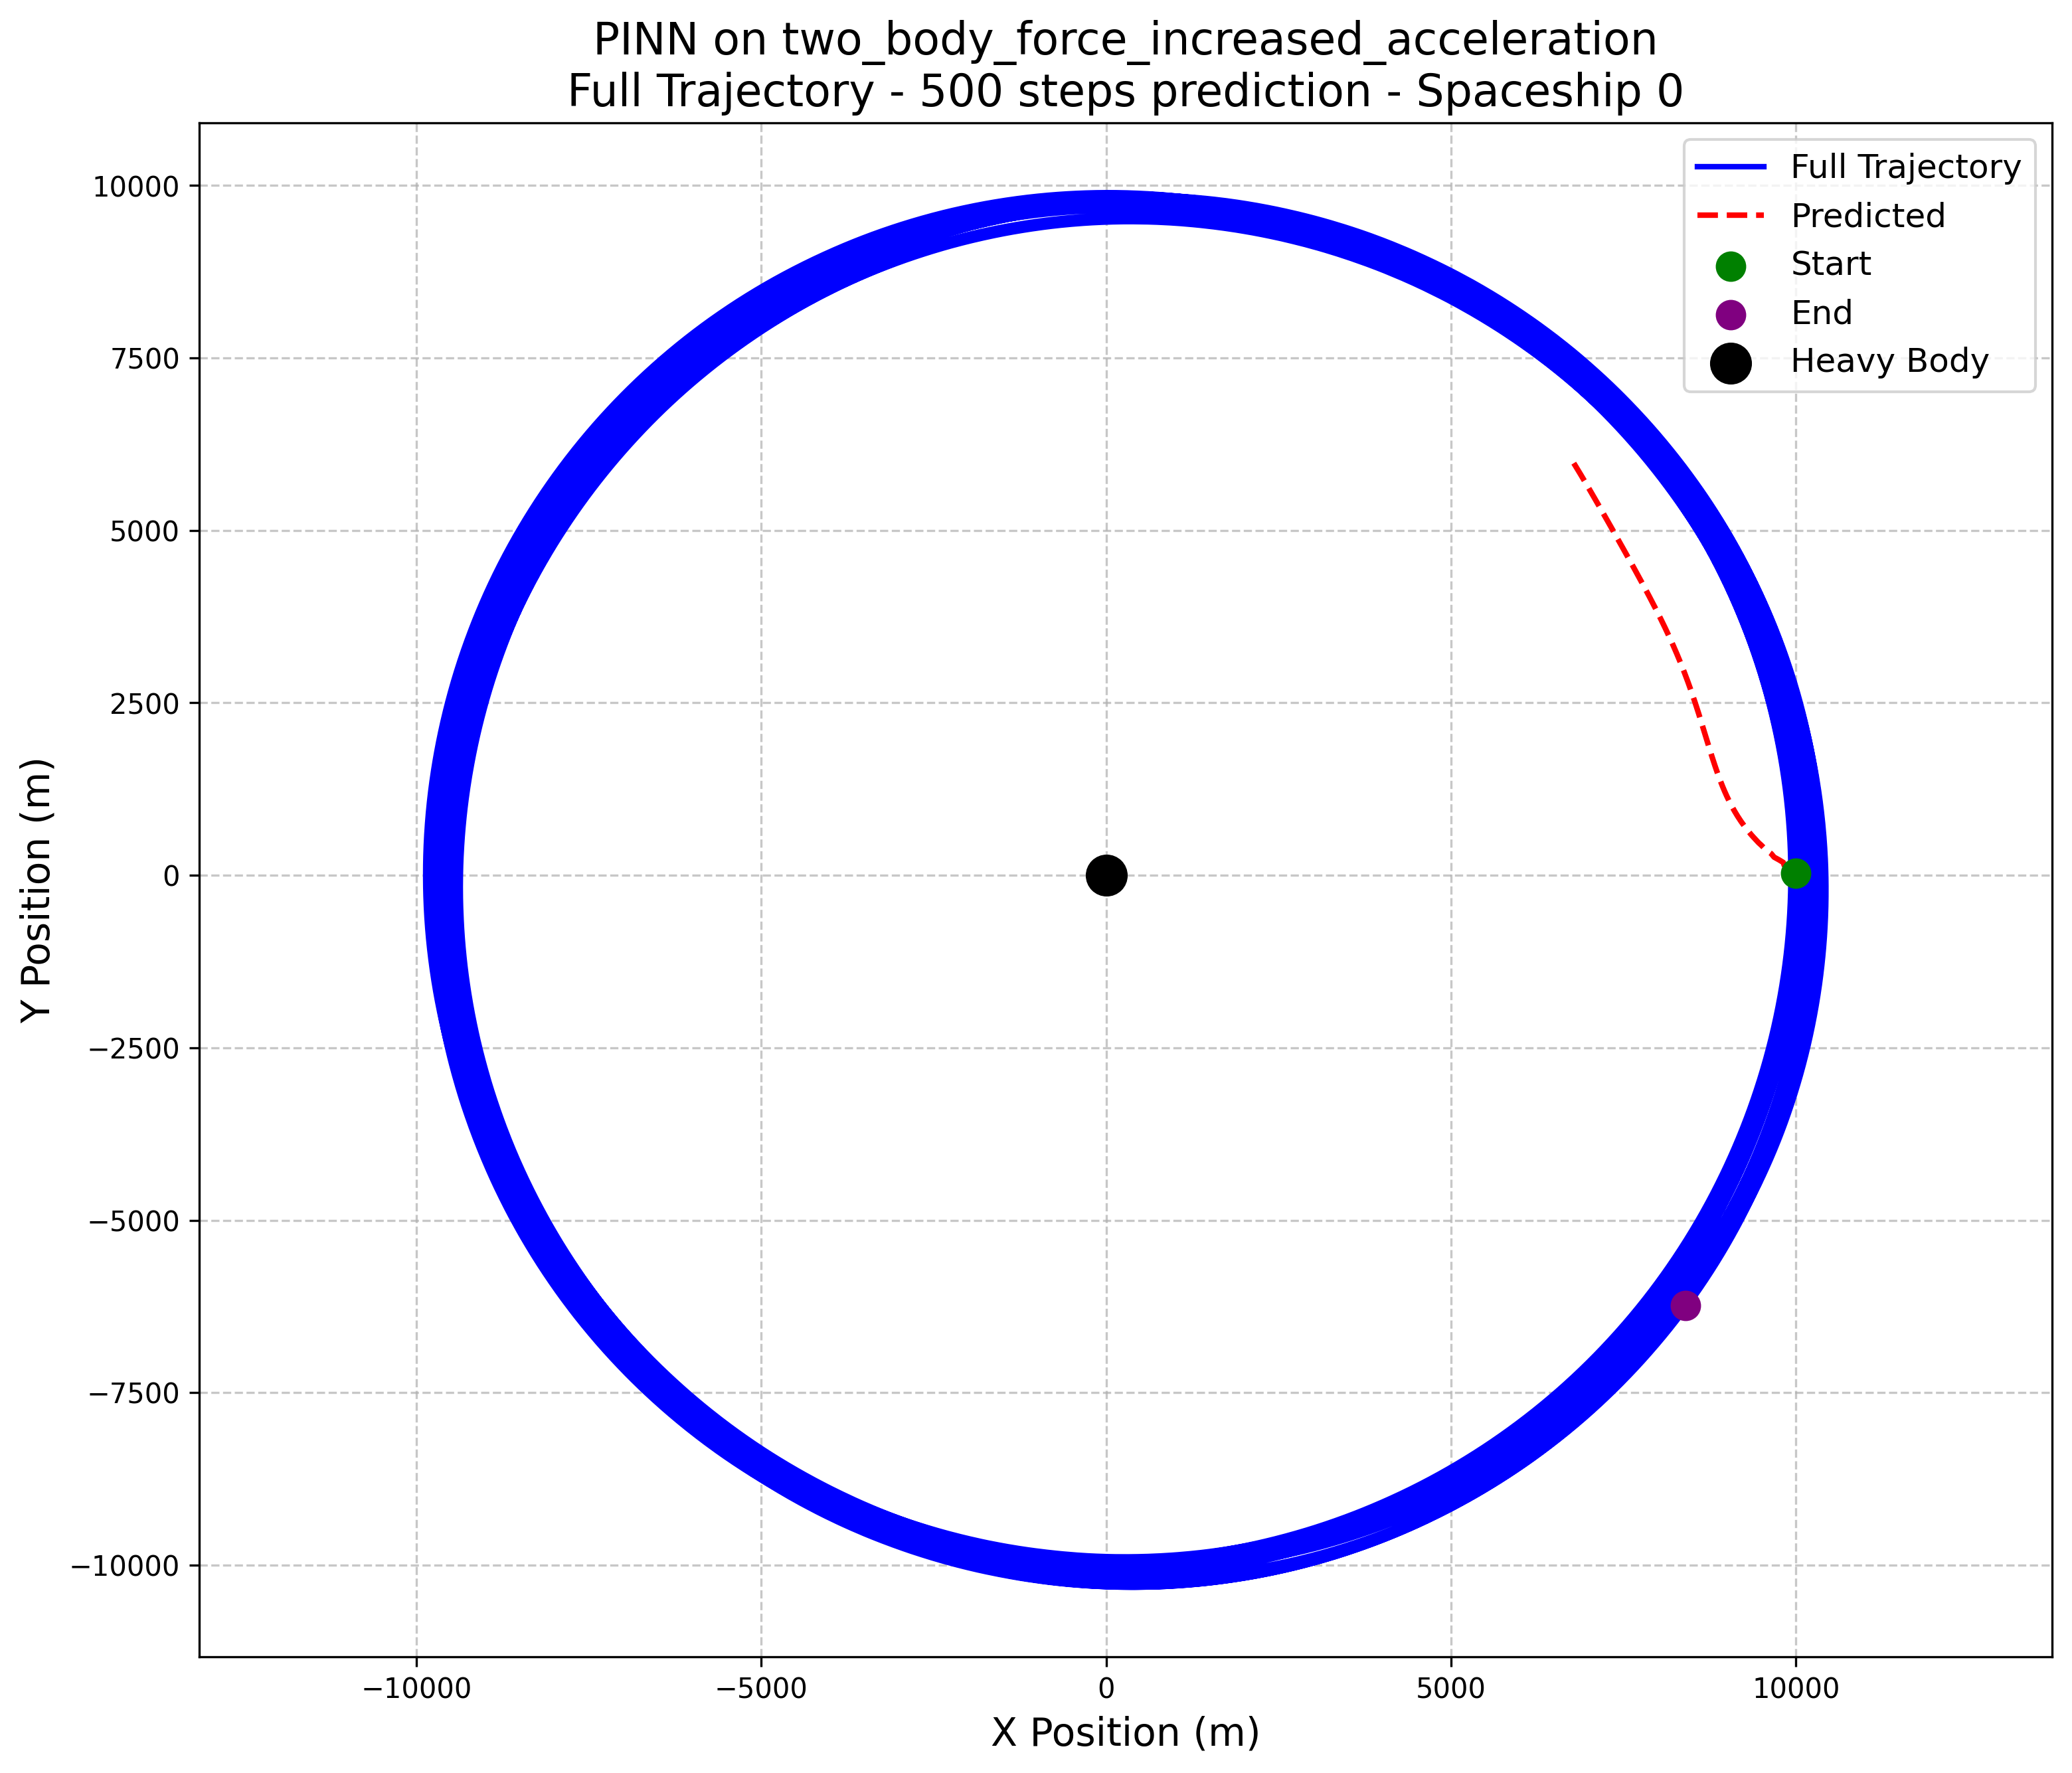
\includegraphics[width=0.27\textwidth]{../inference_results/val/PINN/two_body_force_increased_acceleration/500/full_trajectory_spaceship_0.png} &
      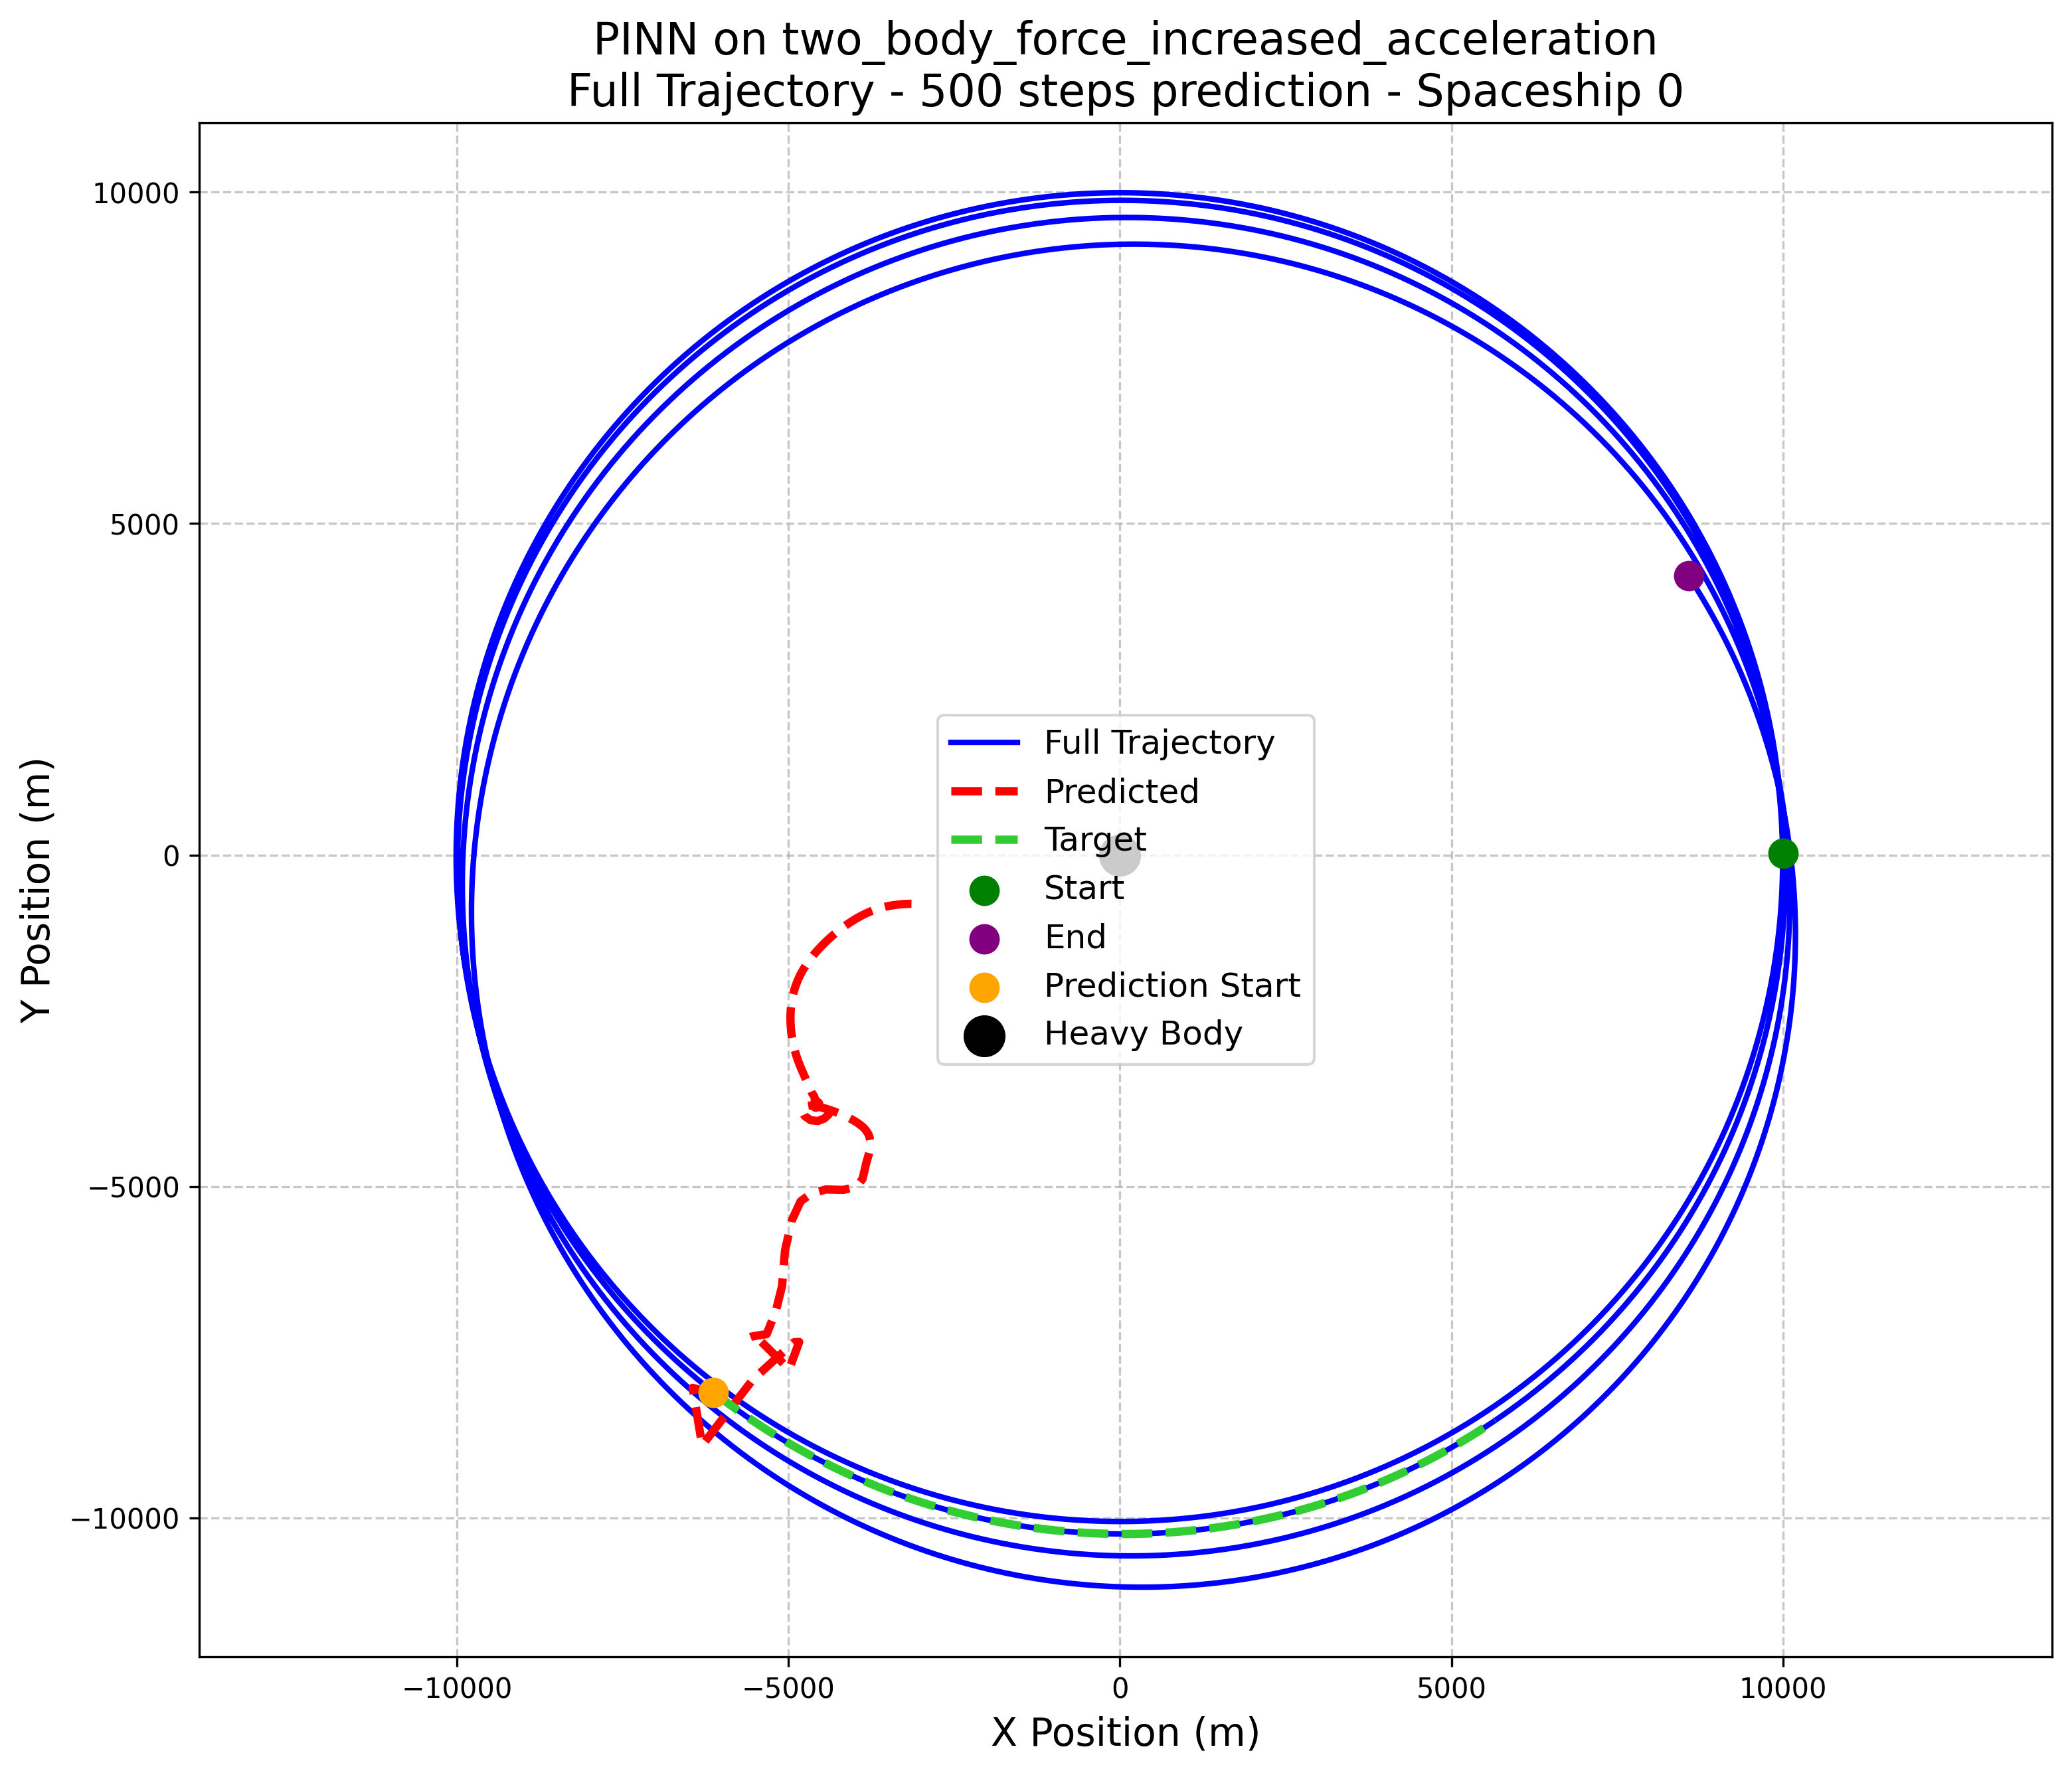
\includegraphics[width=0.27\textwidth]{../inference_results/test/PINN/two_body_force_increased_acceleration/500/full_trajectory_spaceship_0.png}
  \end{tabular}
\end{figure}


\section{Three-Body Problem Trajectory Predictions}
\begin{figure}[H]
  \centering
  \caption{Three-Body Problem: Model Predictions vs. Actual Trajectories}
  \label{fig:three_body_predictions}
  \begin{tabular}{cccc}
      & Train & Validation & Test \\
      MLP &
      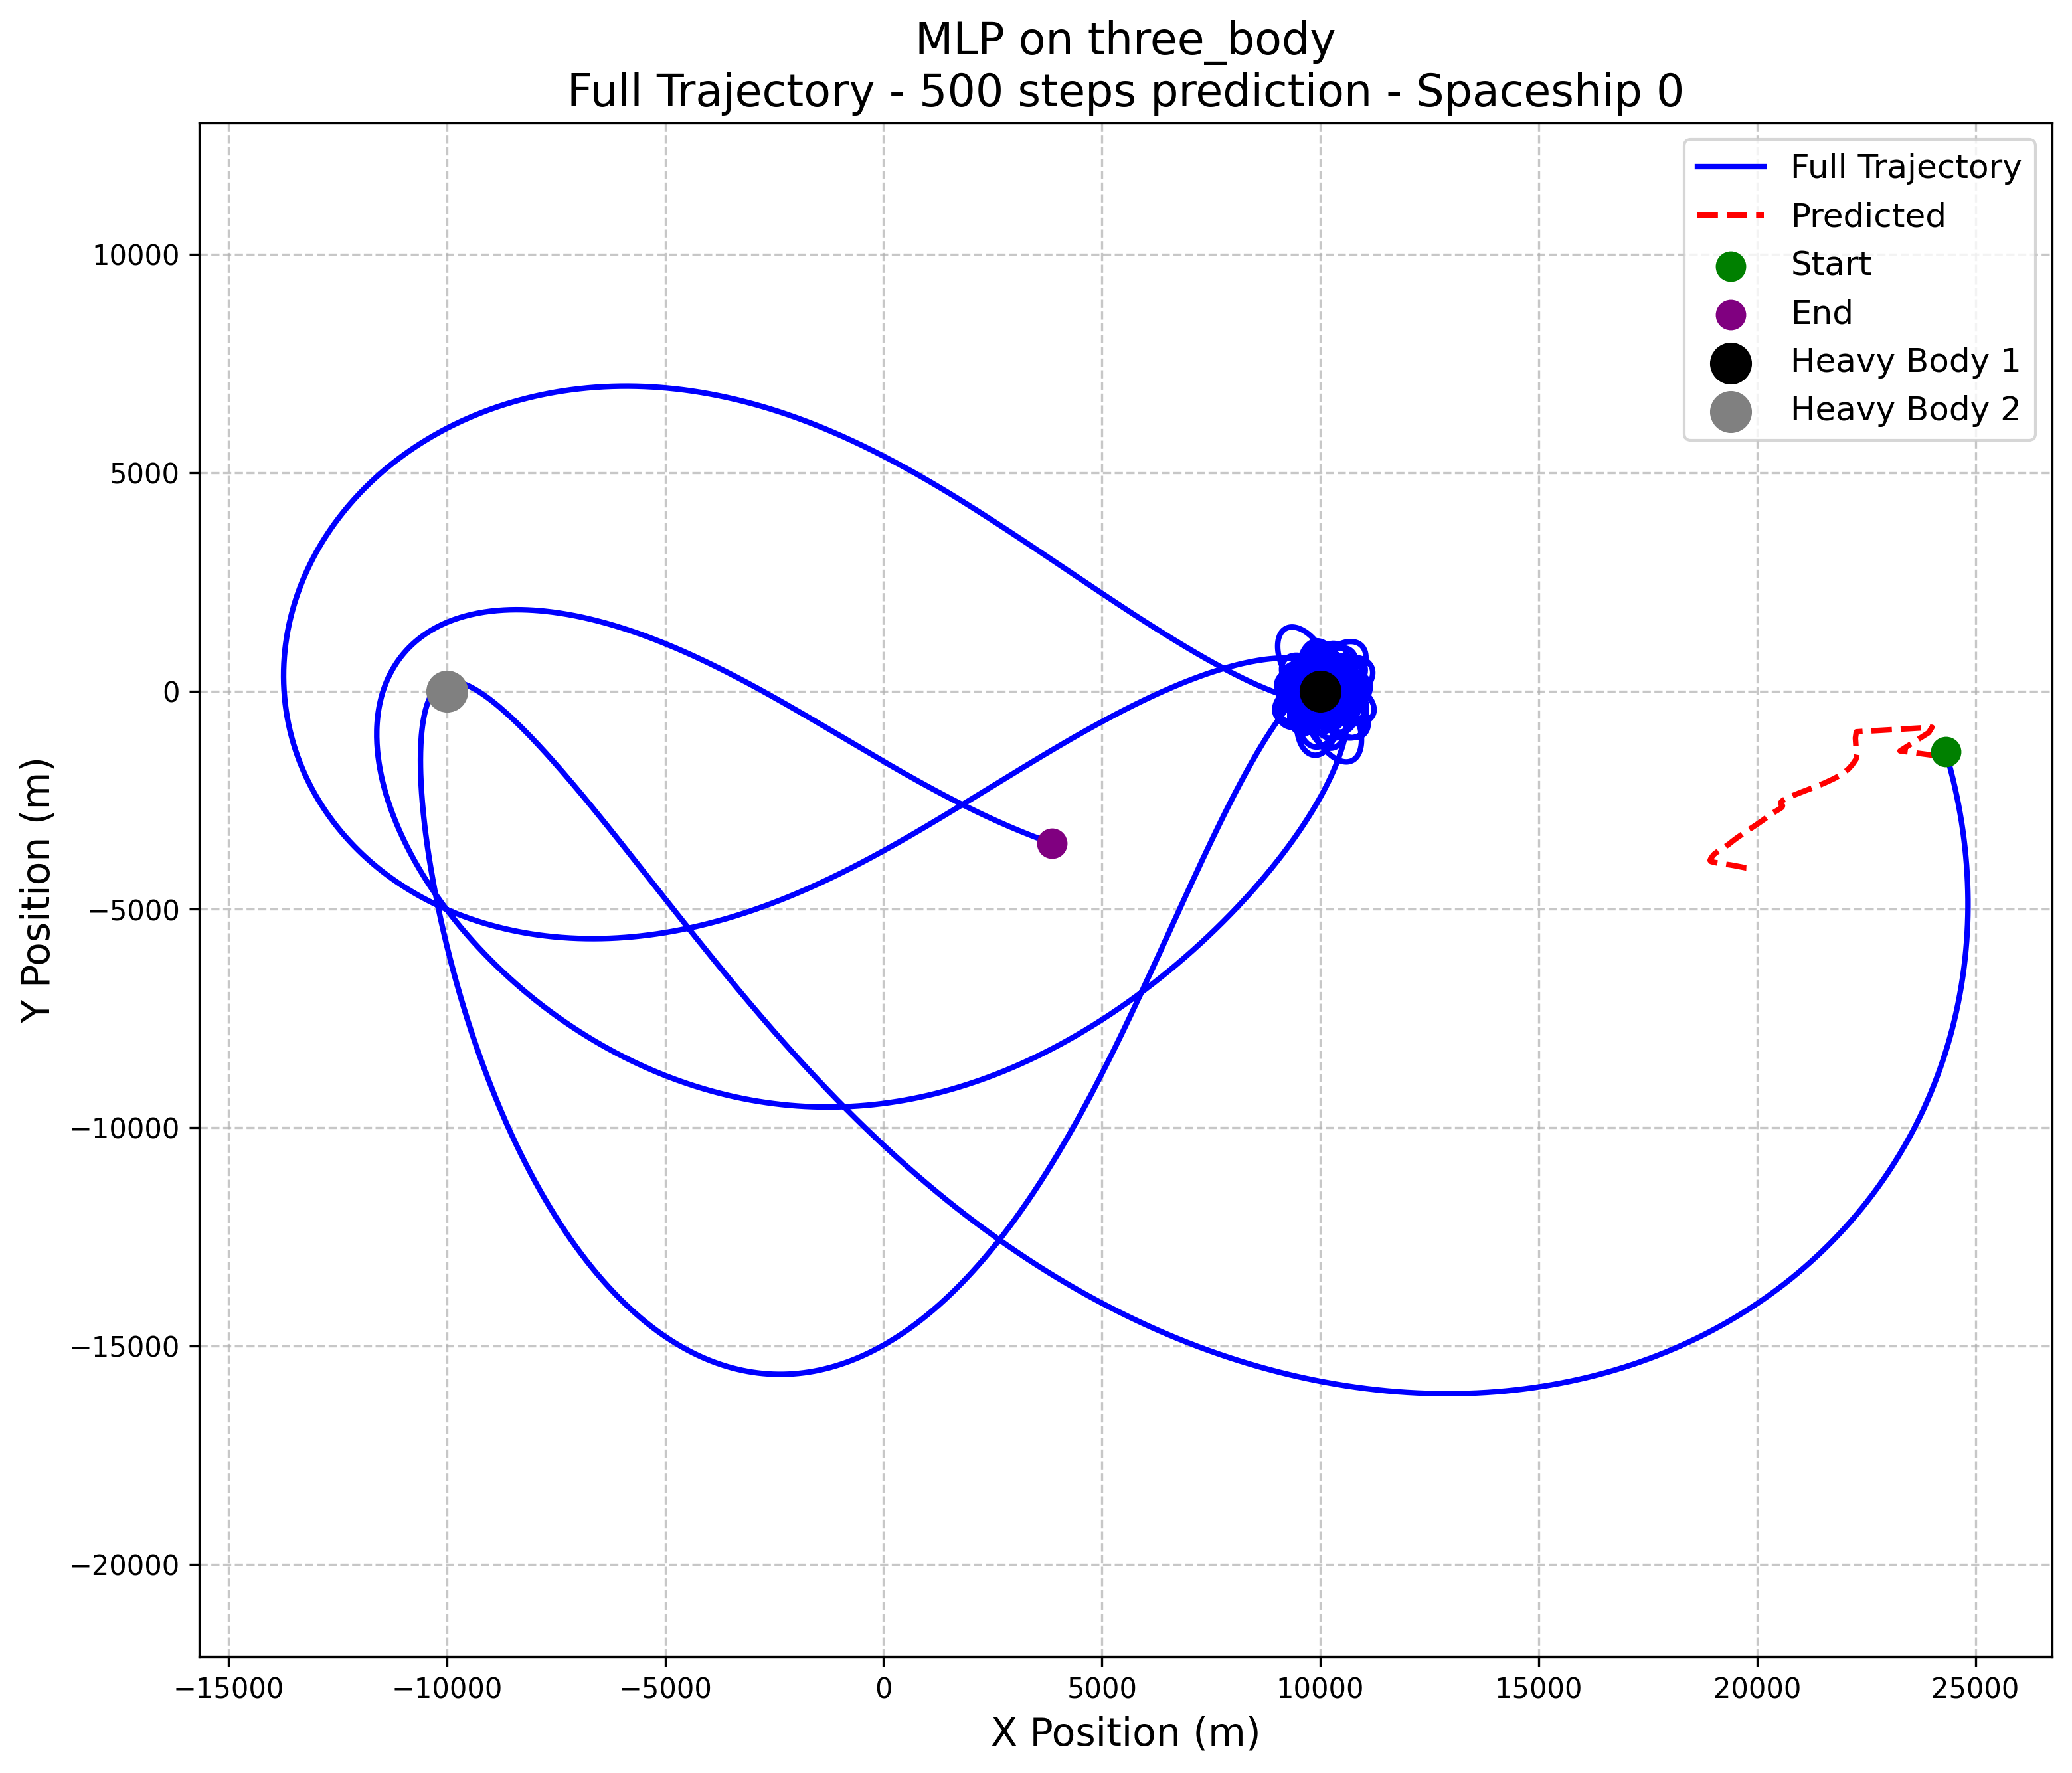
\includegraphics[width=0.27\textwidth]{../inference_results/train/MLP/three_body/500/full_trajectory_spaceship_0.png} &
      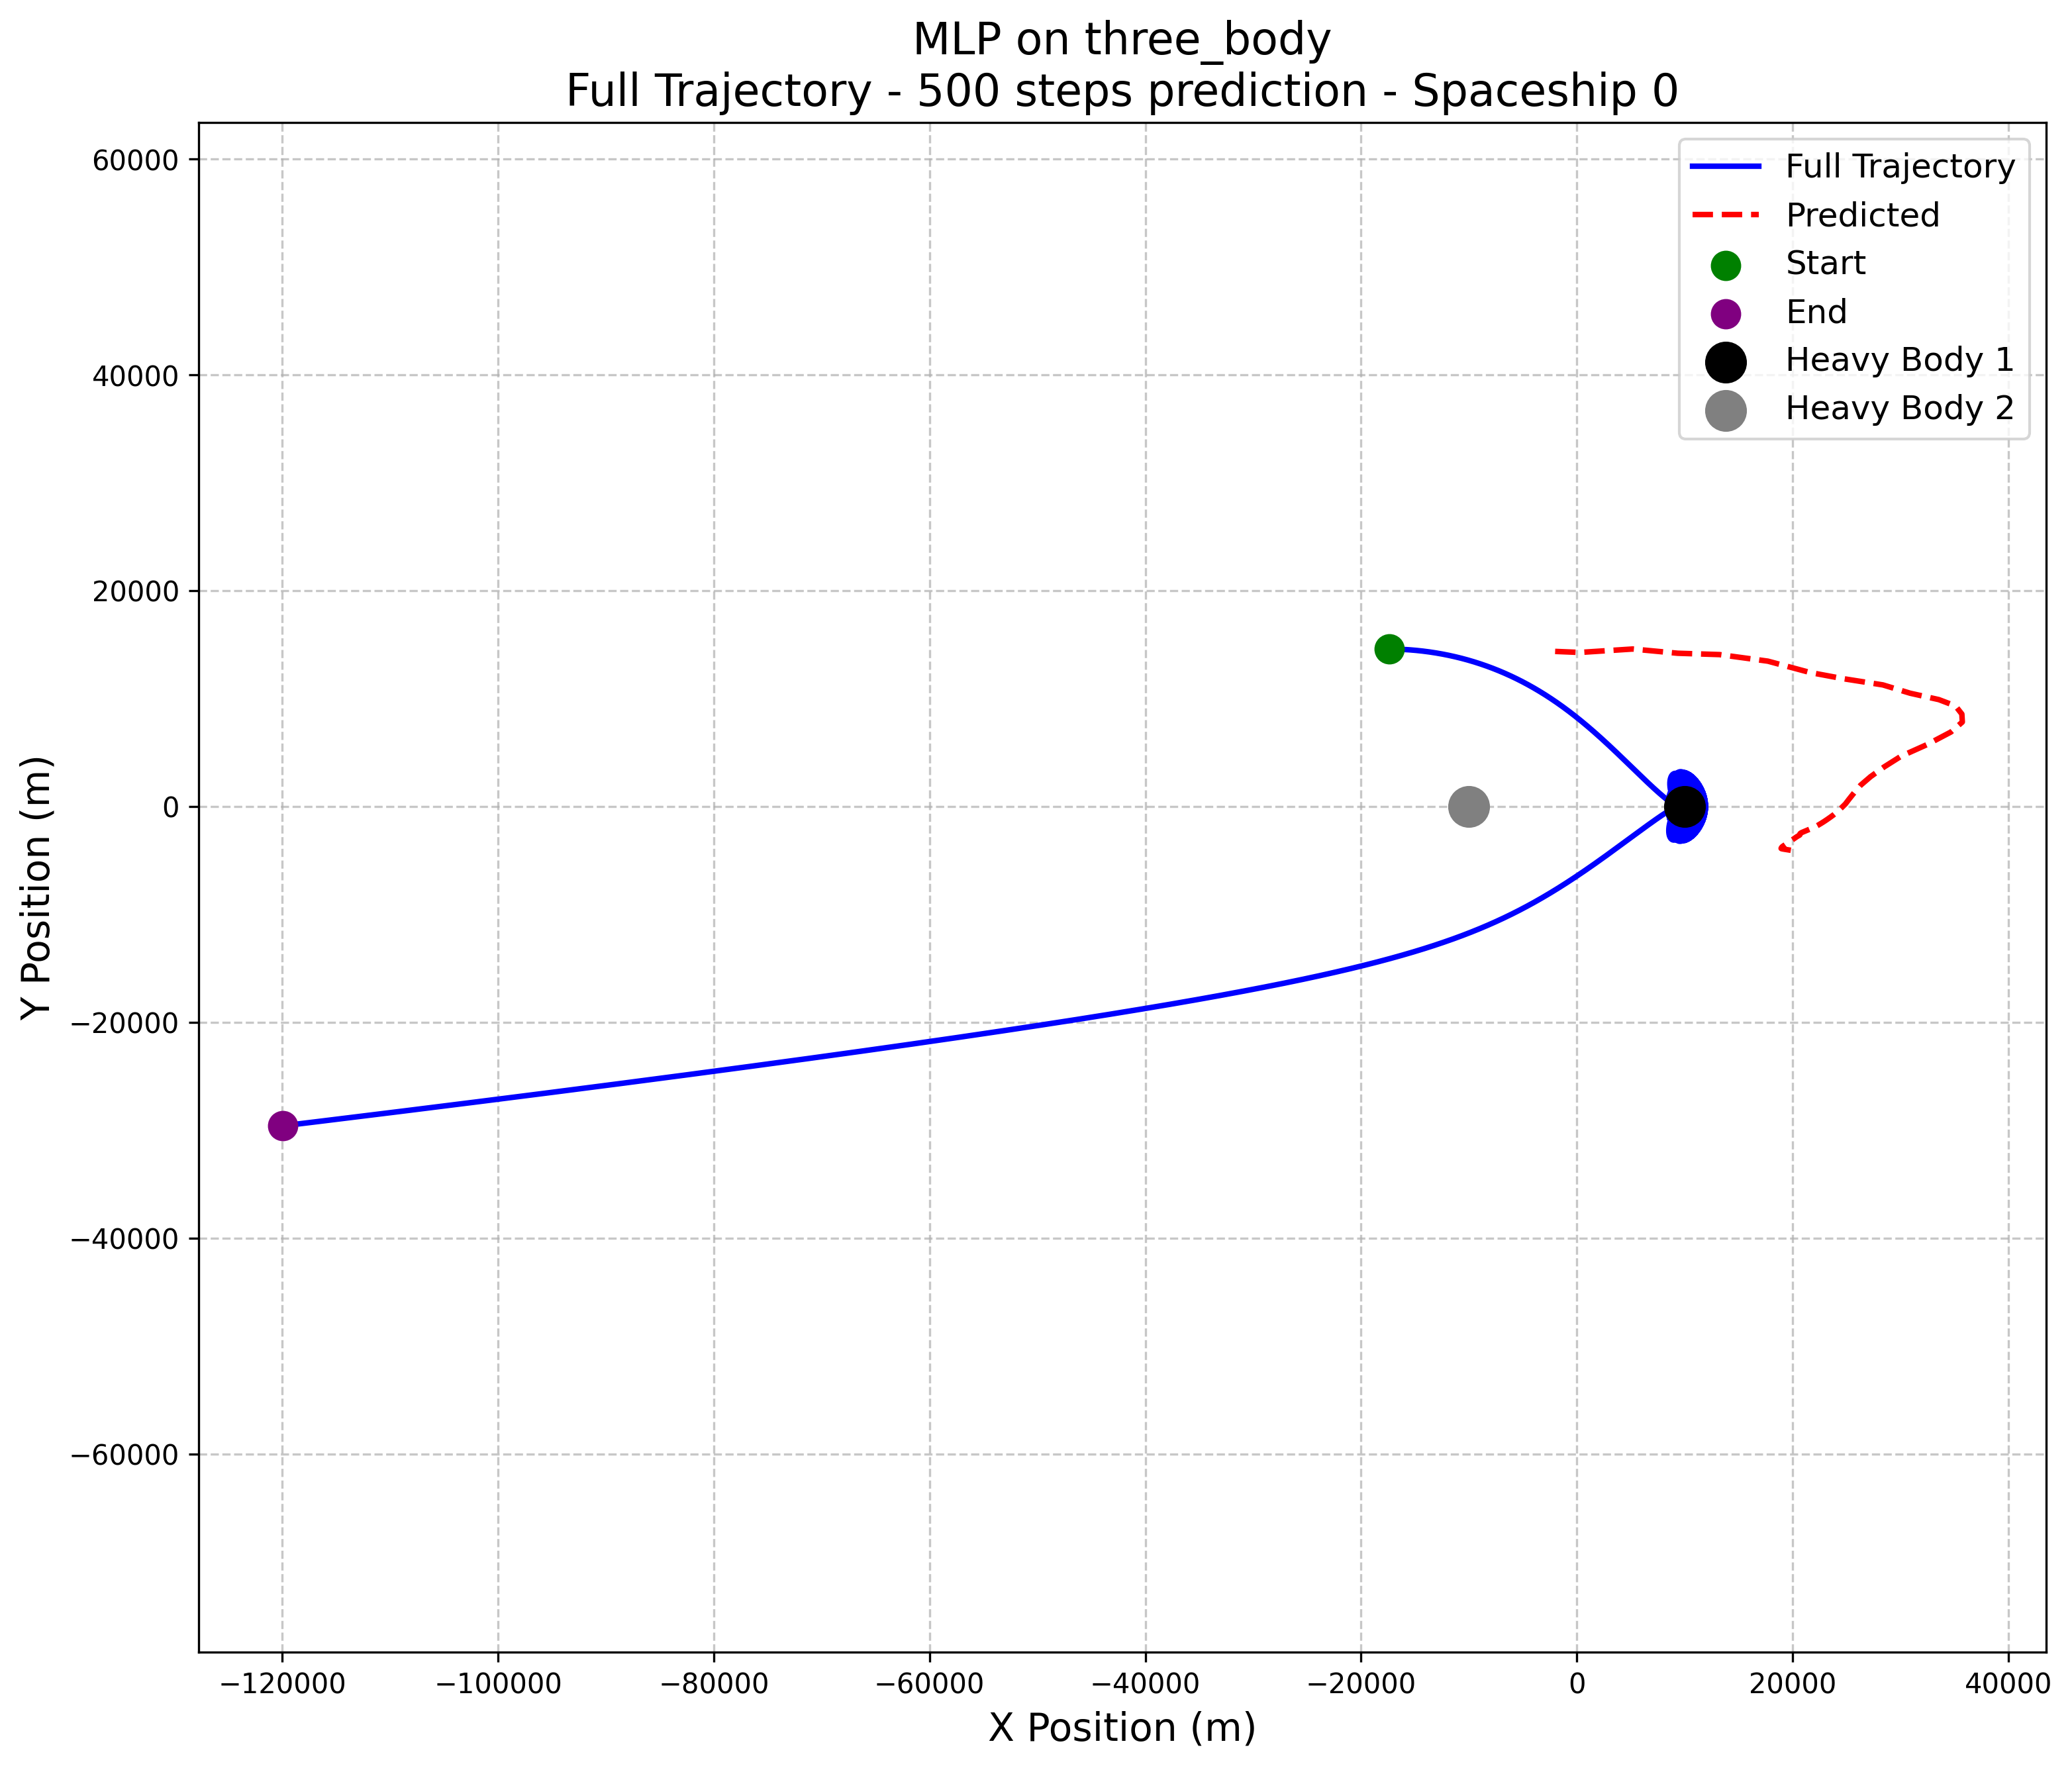
\includegraphics[width=0.27\textwidth]{../inference_results/val/MLP/three_body/500/full_trajectory_spaceship_0.png} &
      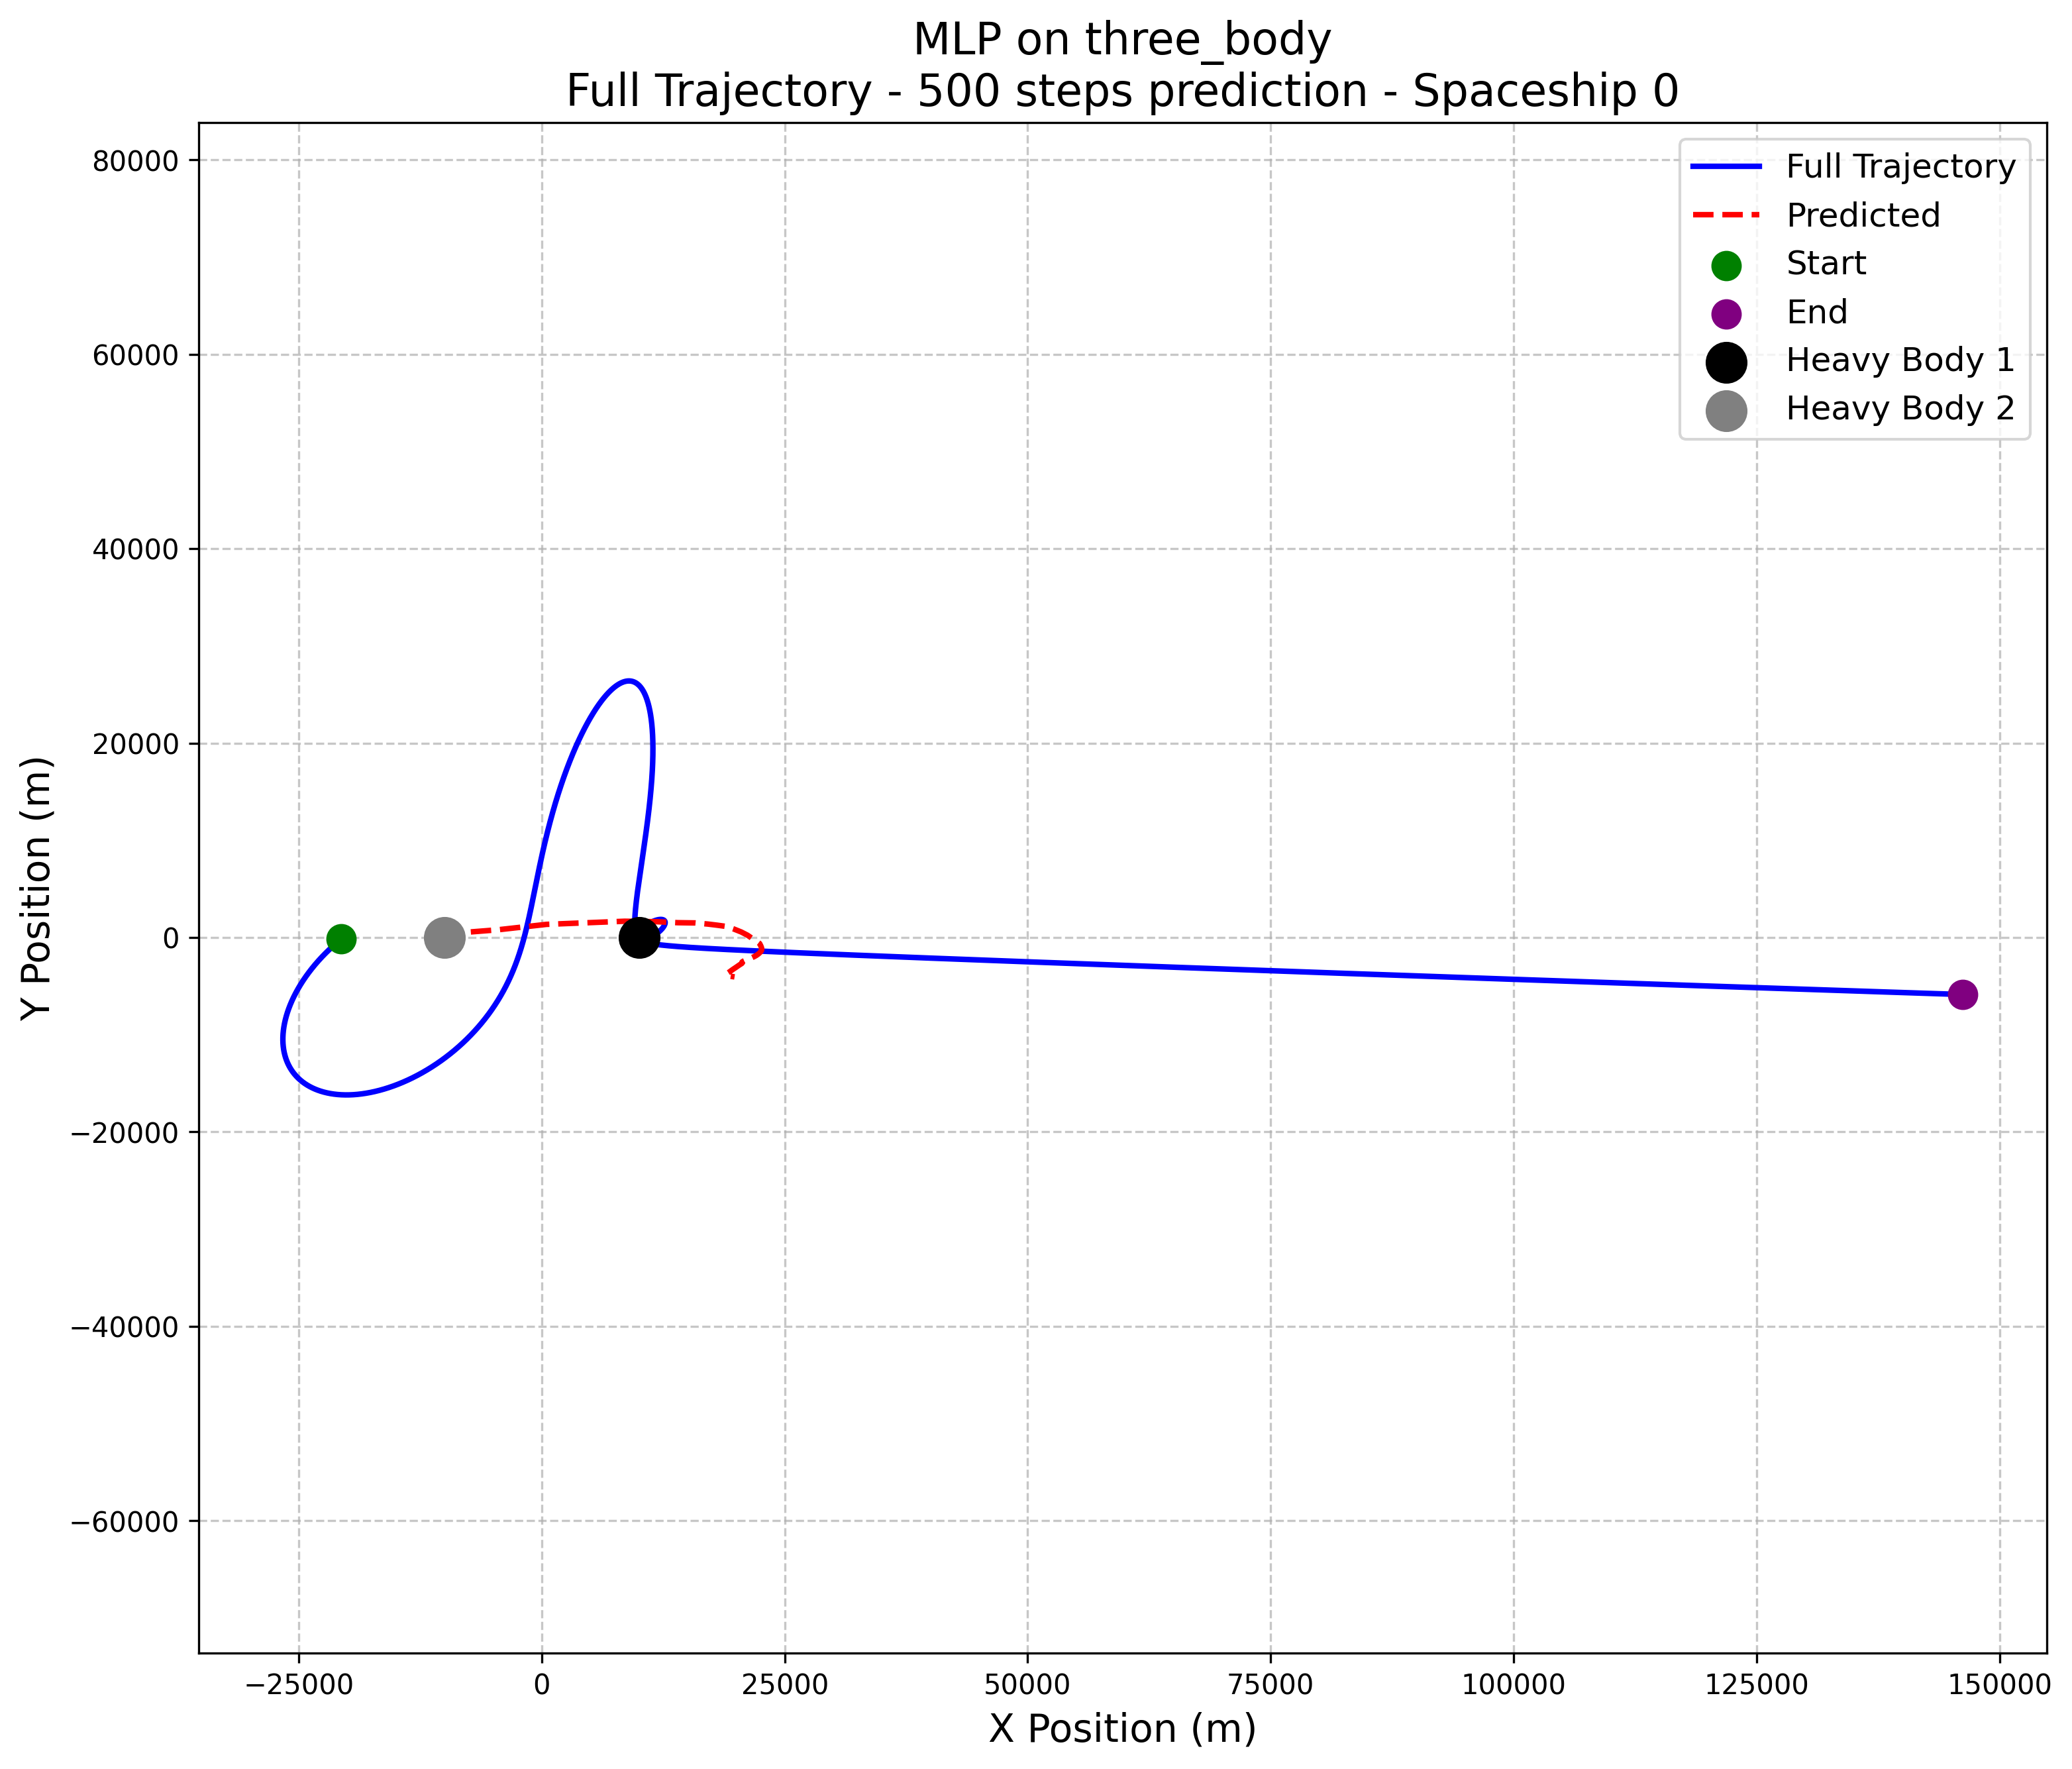
\includegraphics[width=0.27\textwidth]{../inference_results/test/MLP/three_body/500/full_trajectory_spaceship_0.png} \\
      LSTM &
      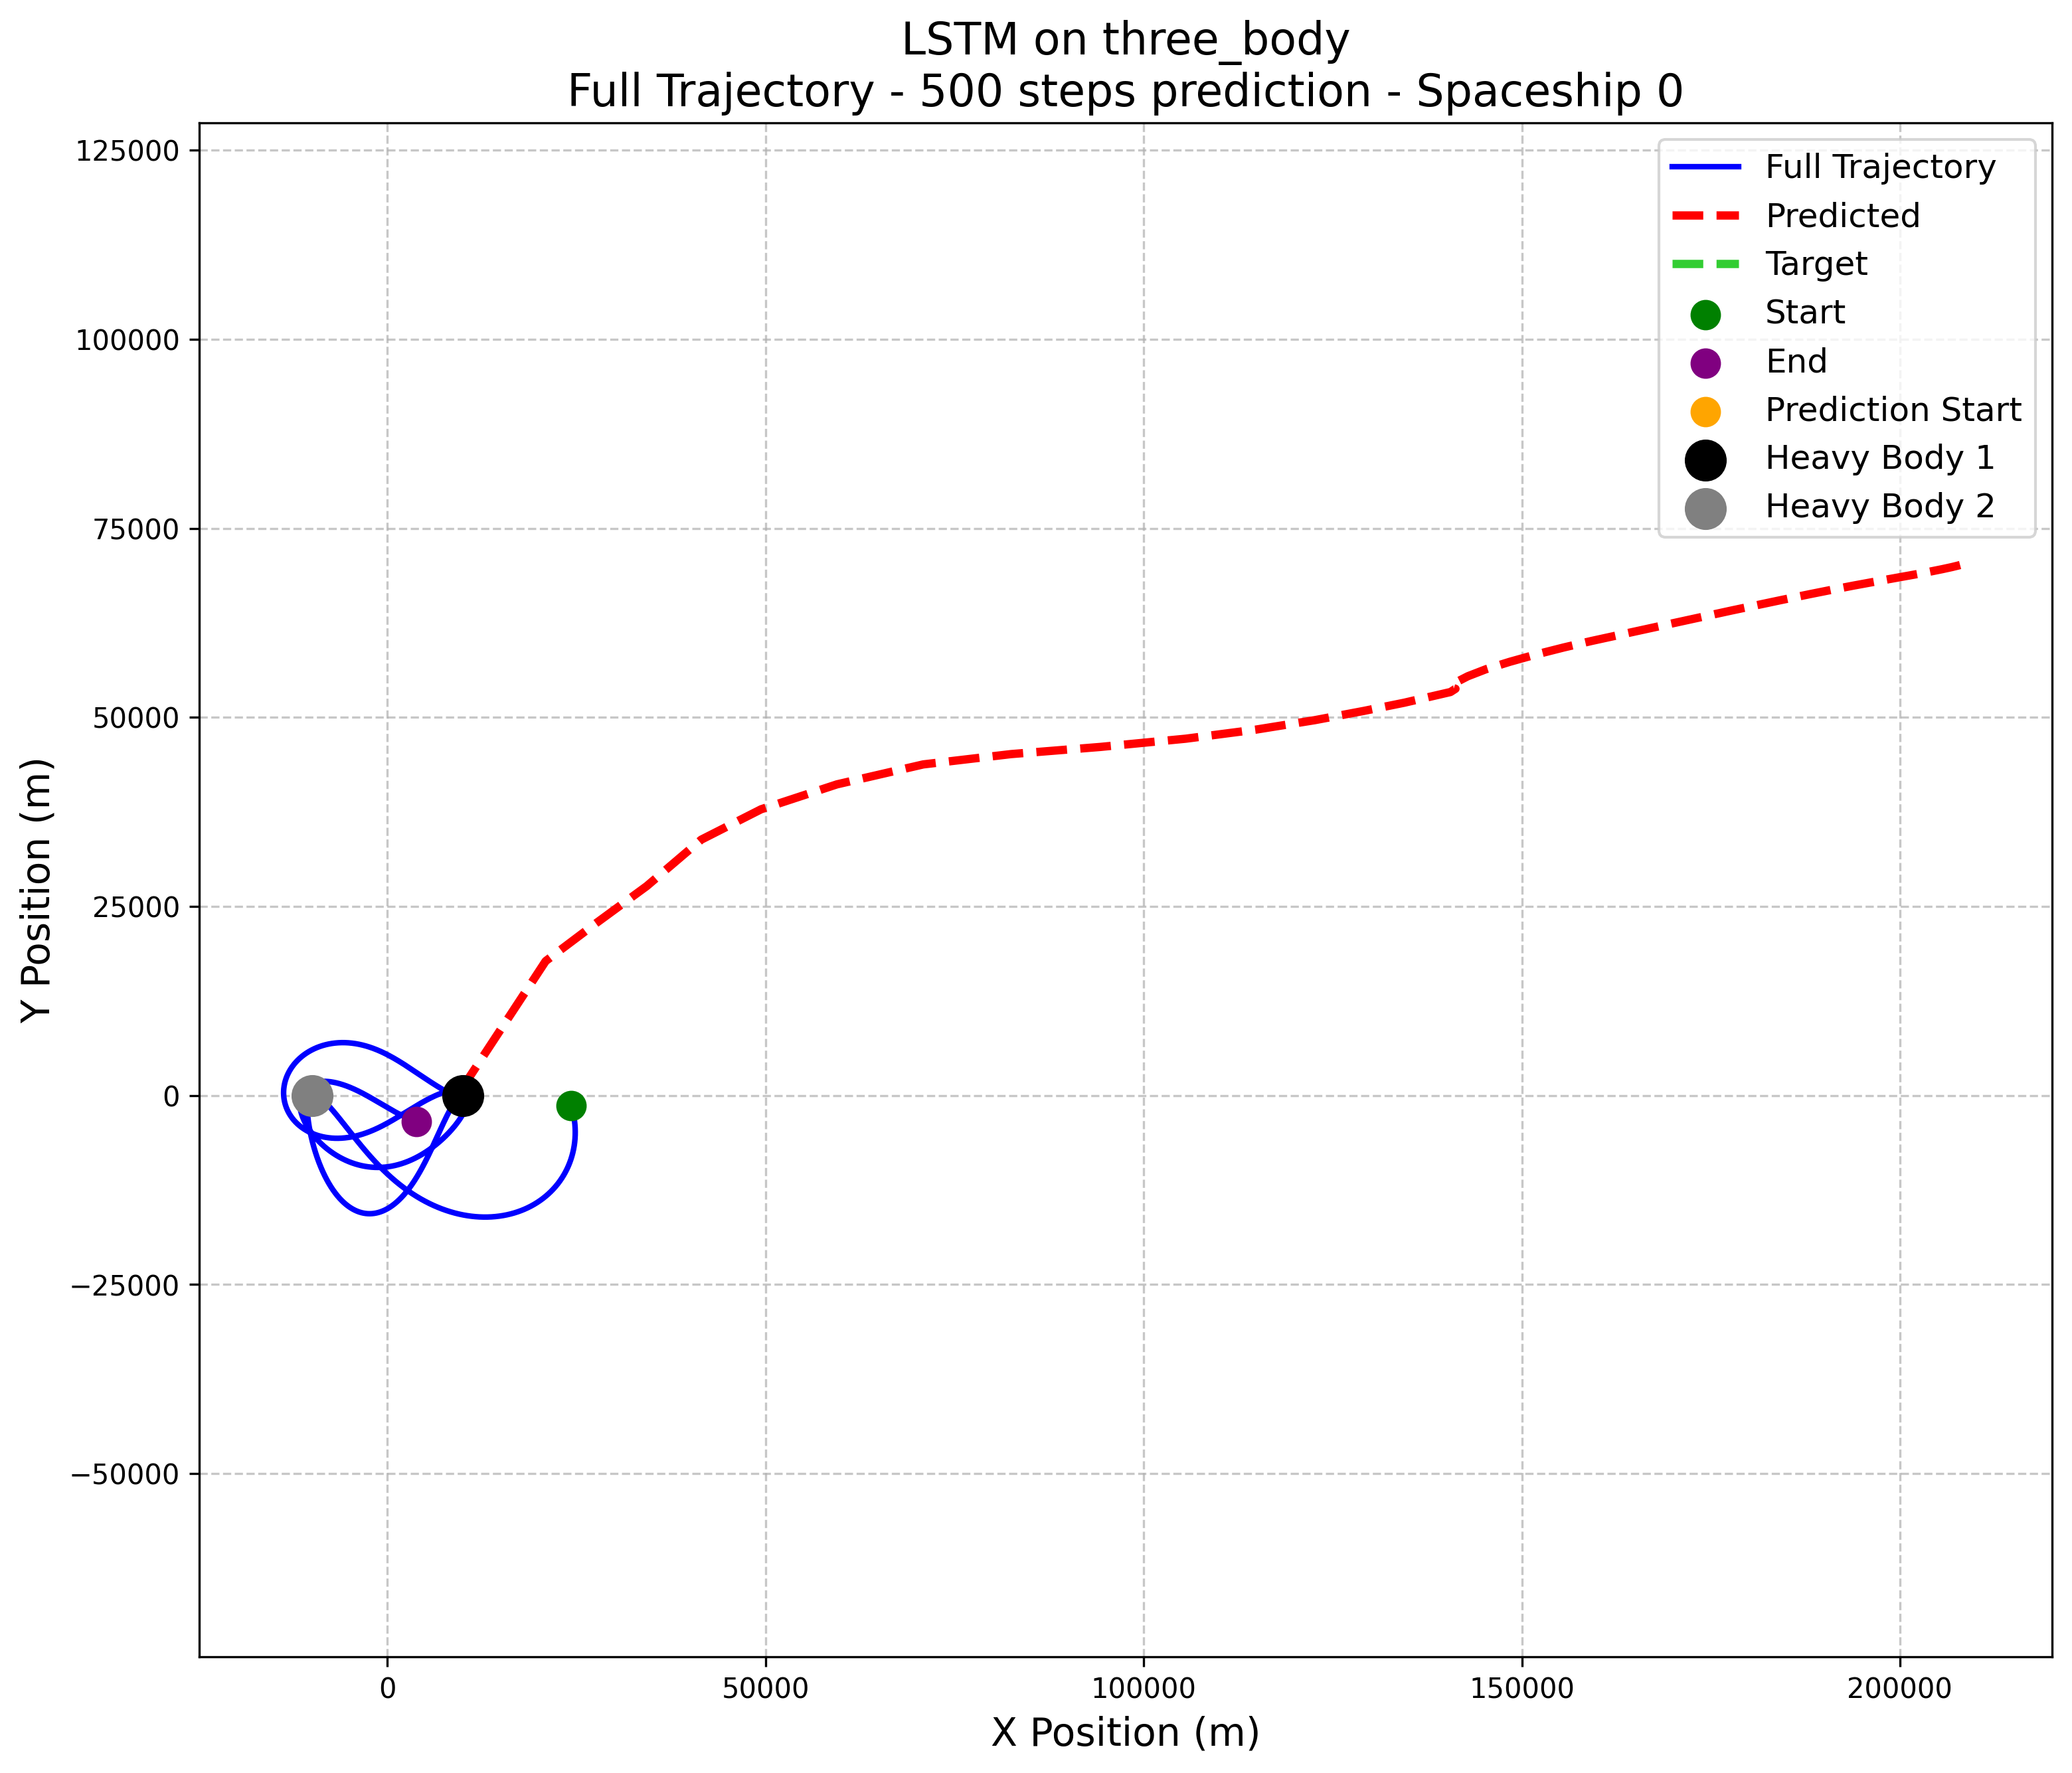
\includegraphics[width=0.27\textwidth]{../inference_results/train/LSTM/three_body/500/full_trajectory_spaceship_0.png} &
      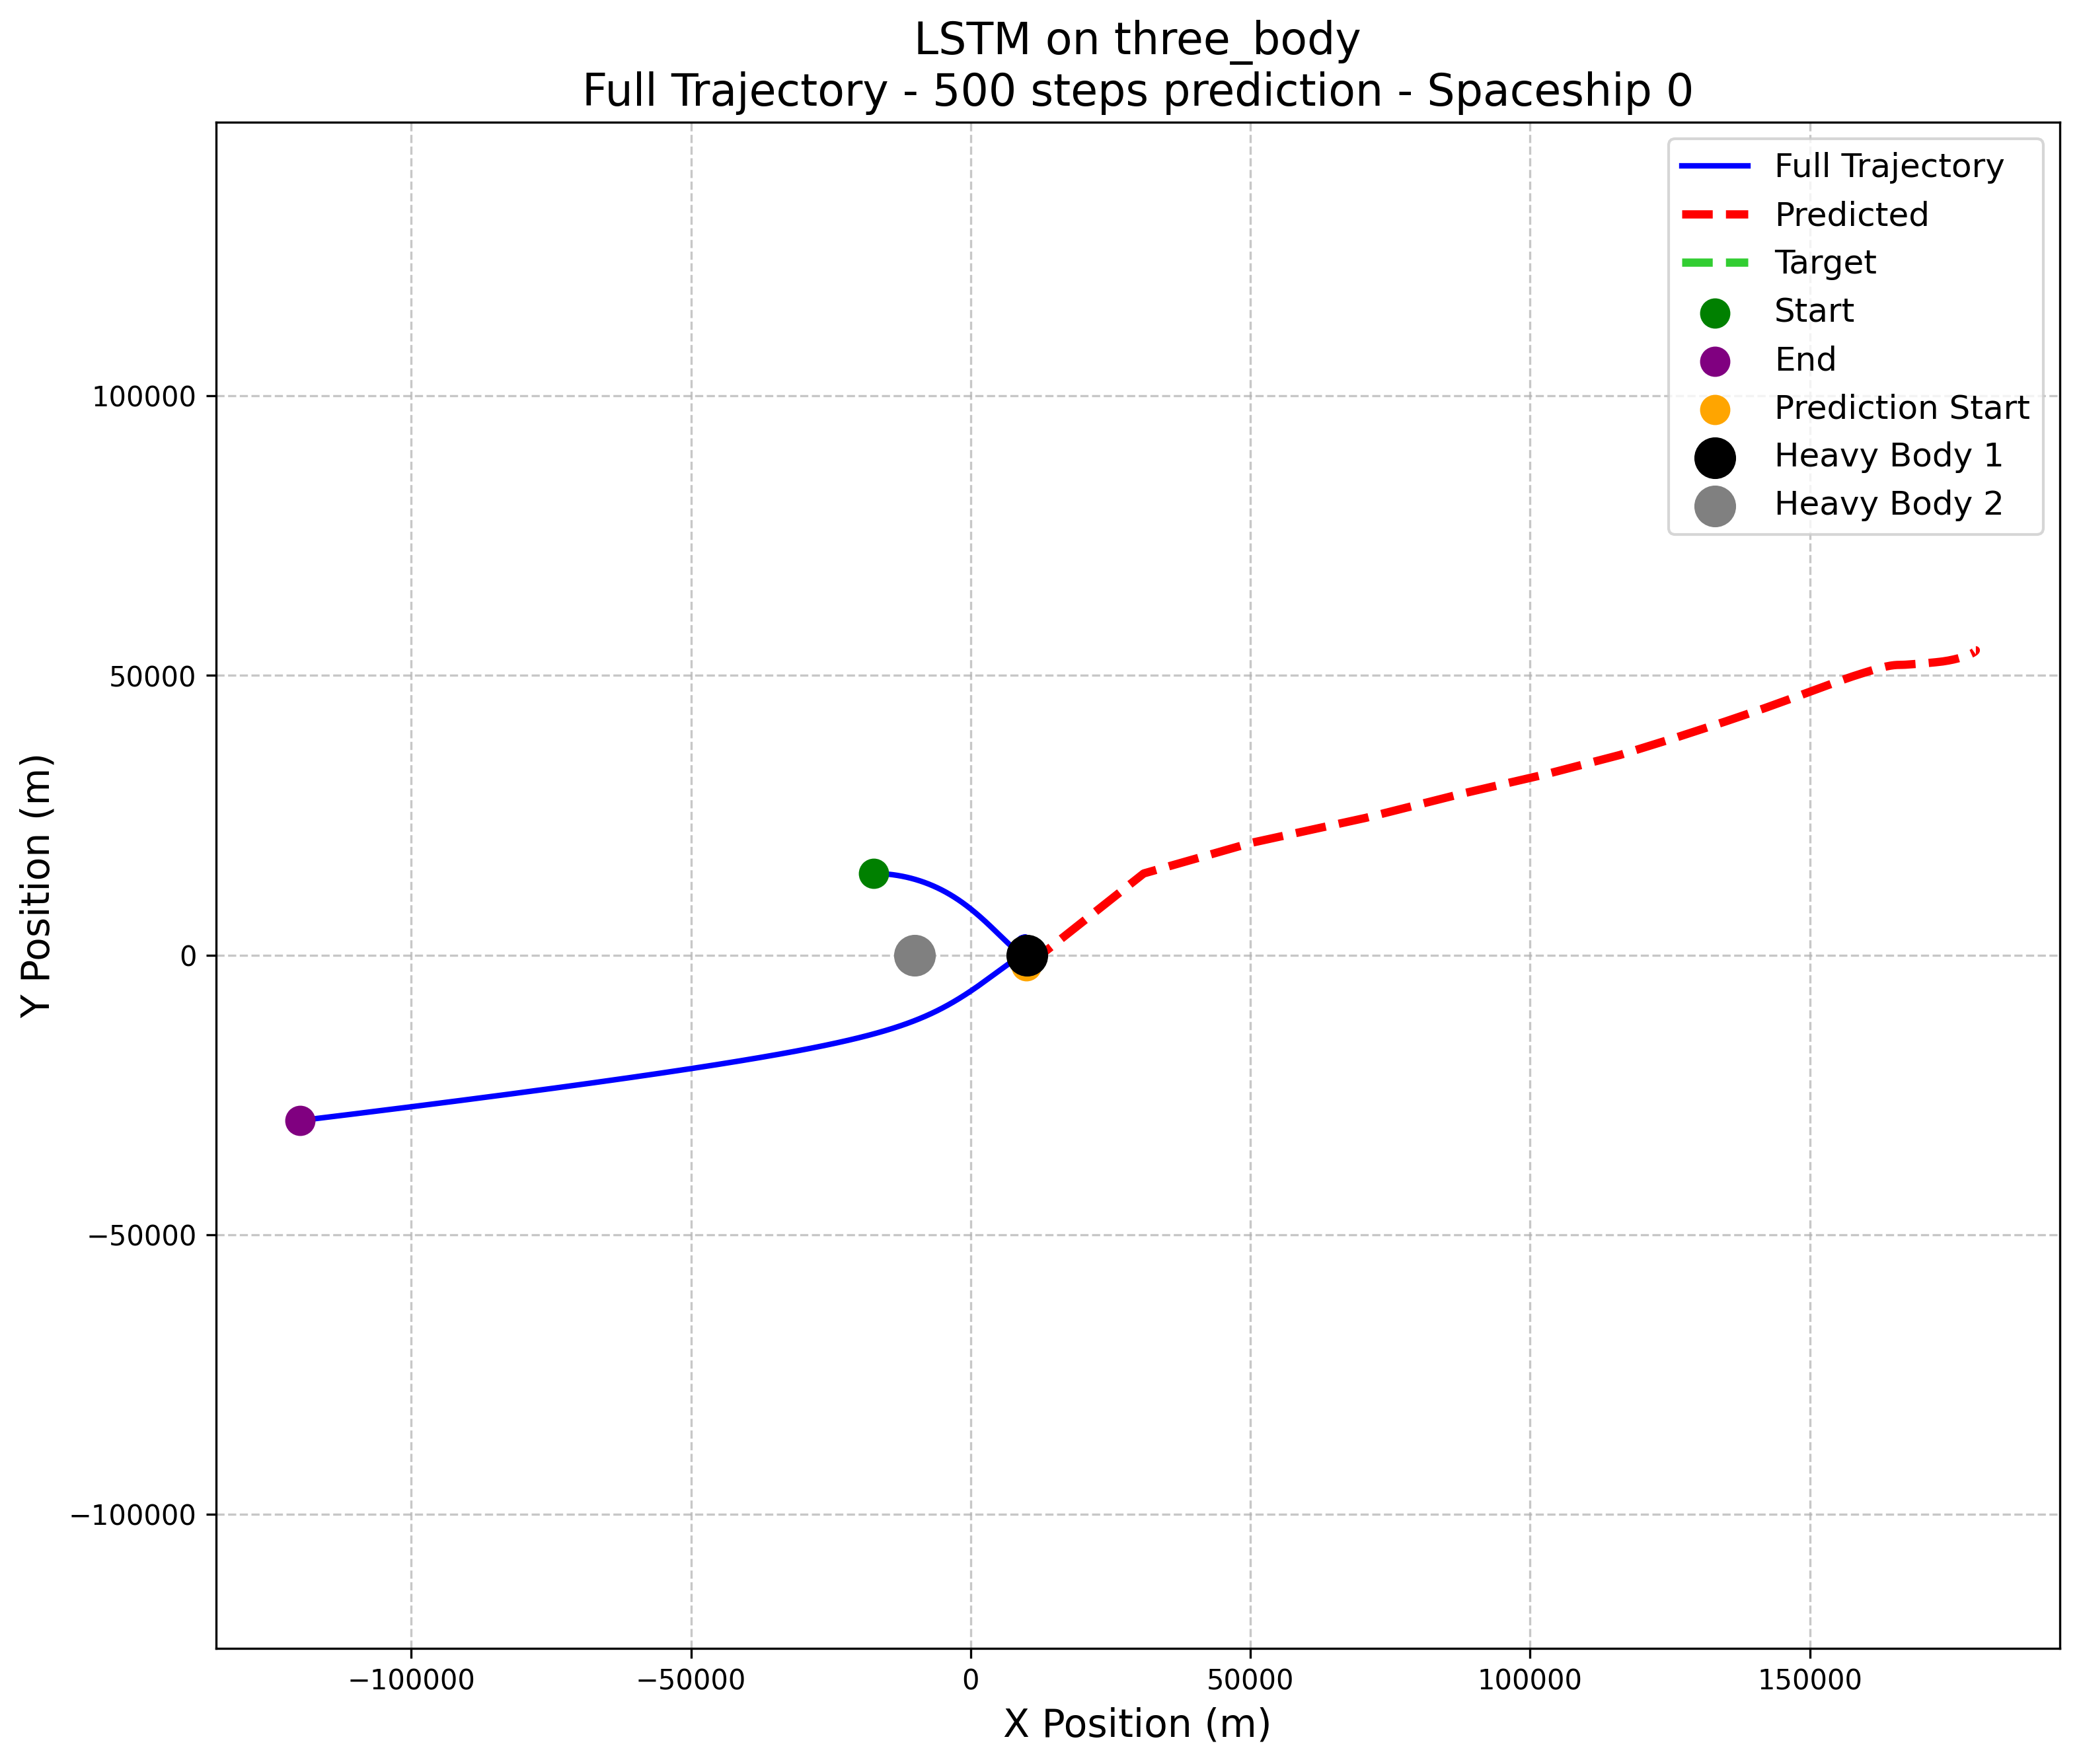
\includegraphics[width=0.27\textwidth]{../inference_results/val/LSTM/three_body/500/full_trajectory_spaceship_0.png} &
      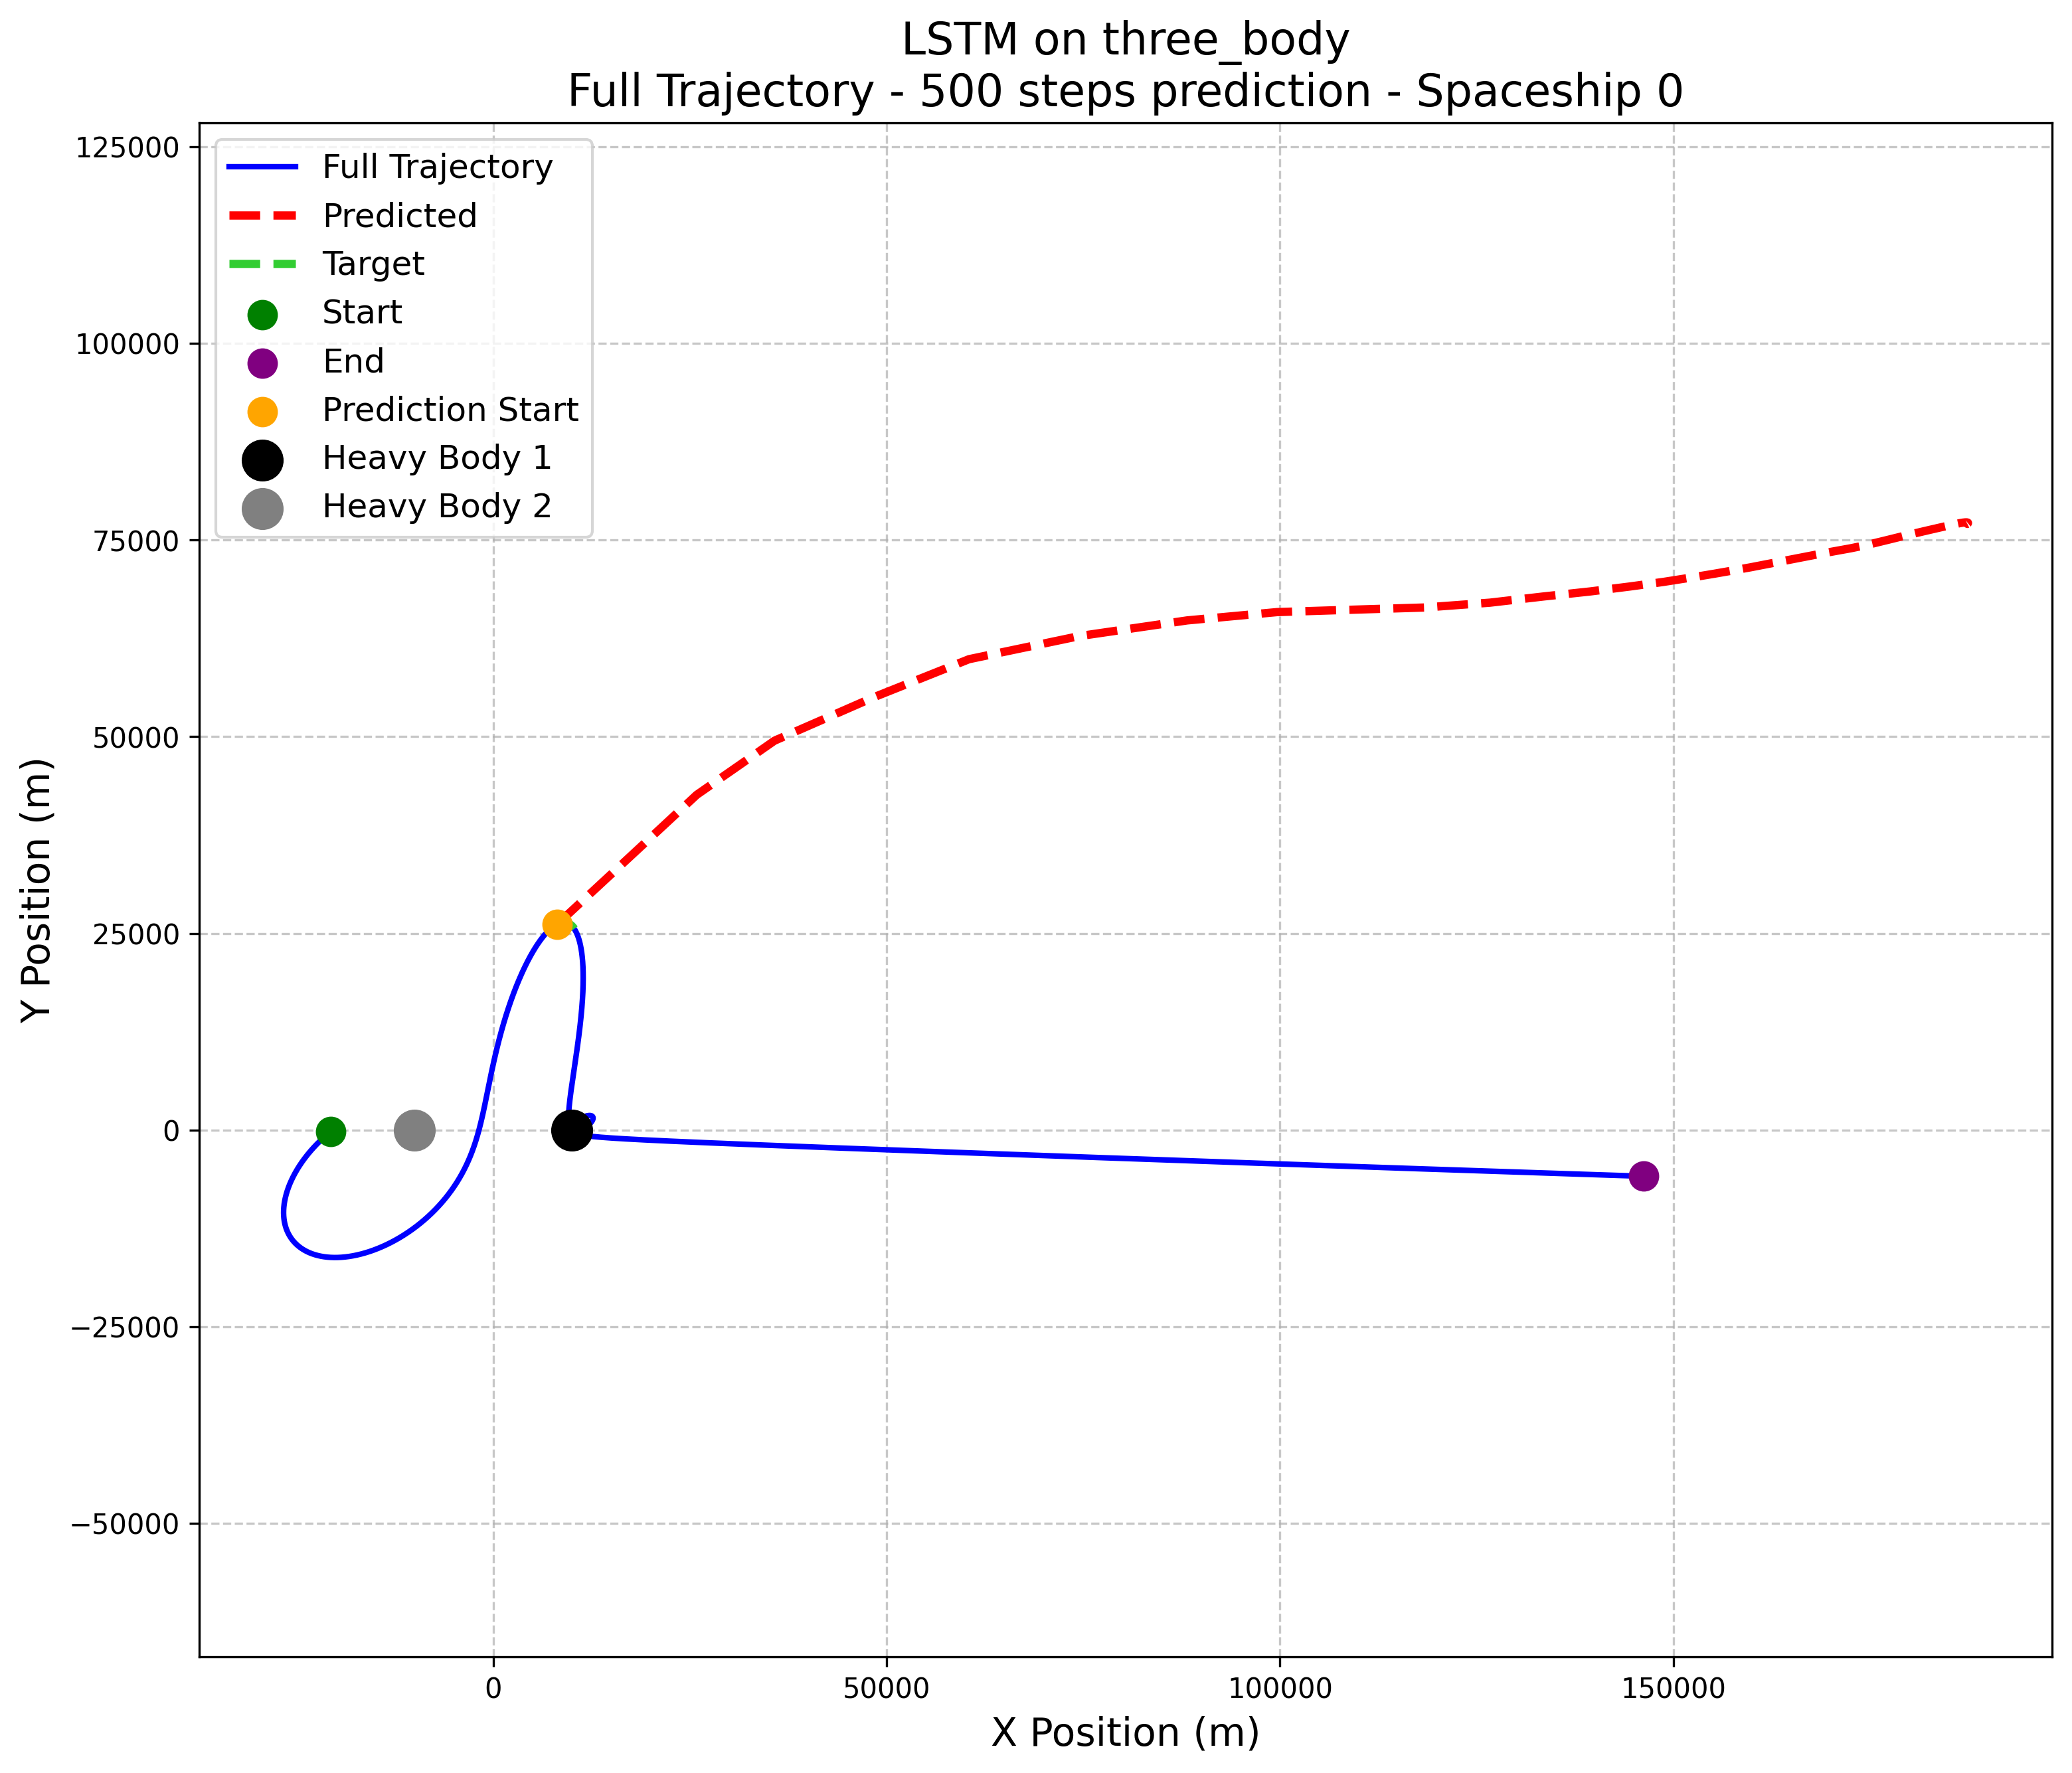
\includegraphics[width=0.27\textwidth]{../inference_results/test/LSTM/three_body/500/full_trajectory_spaceship_0.png} \\
      PINN &
      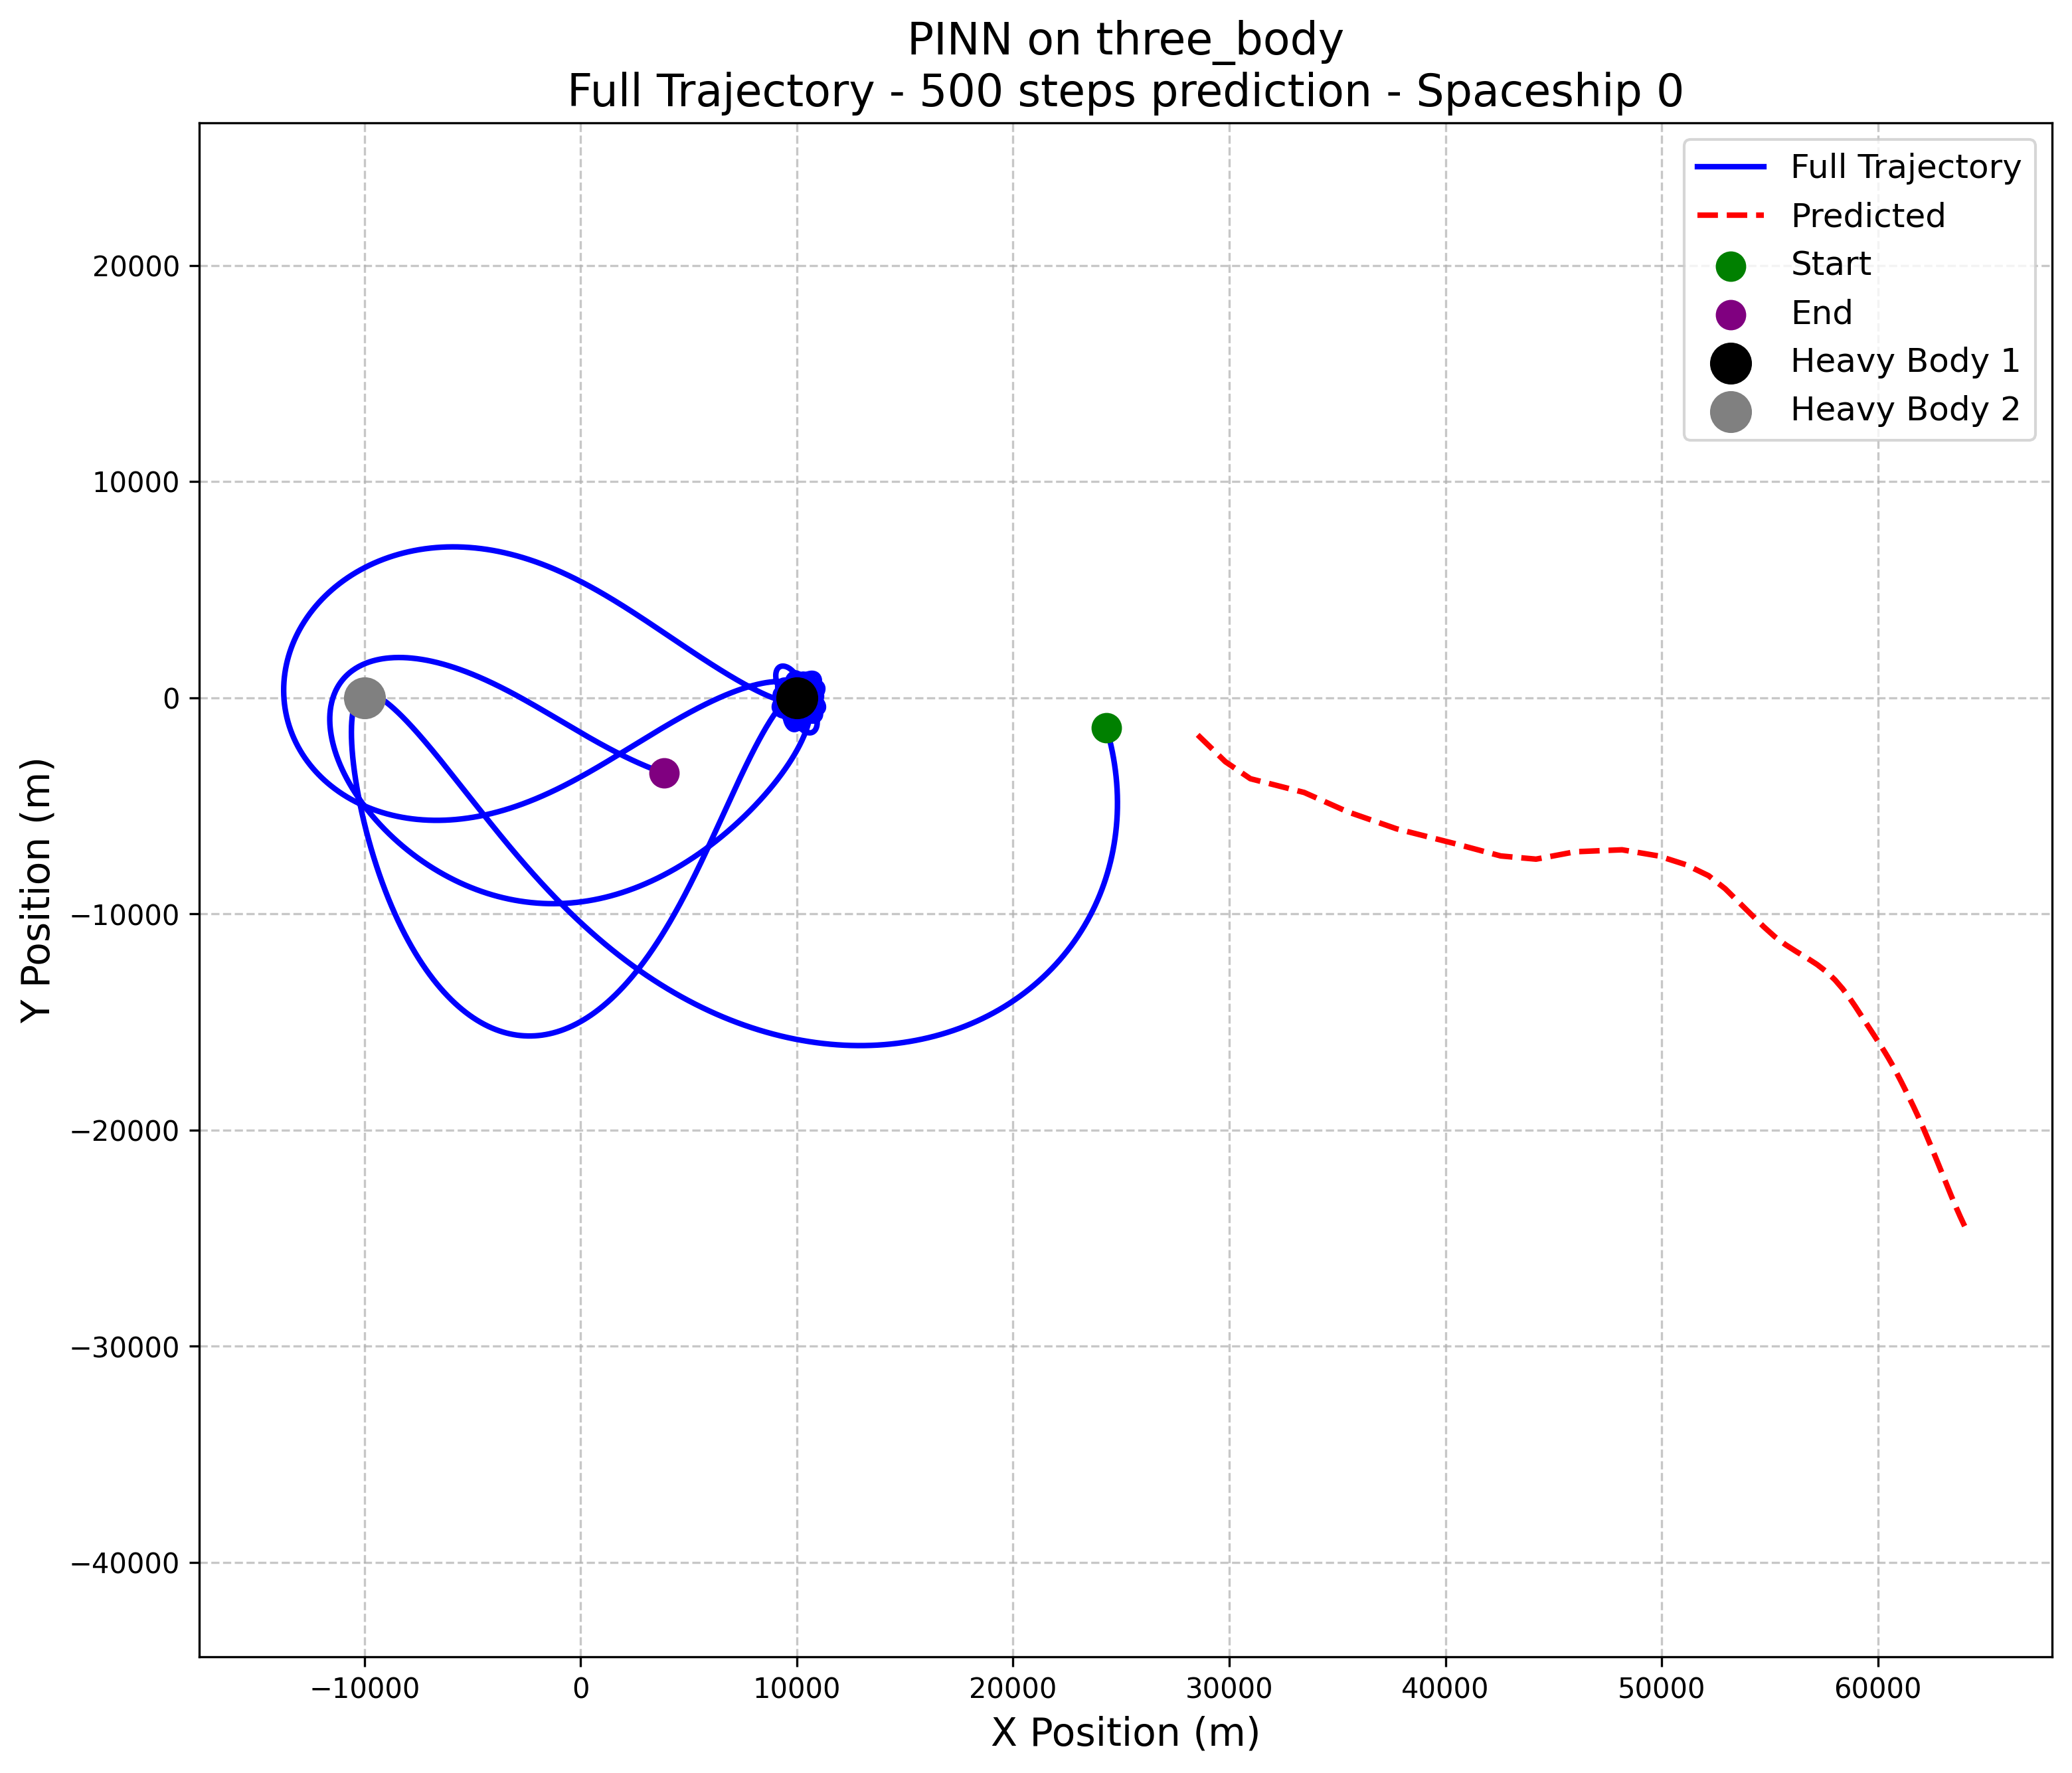
\includegraphics[width=0.27\textwidth]{../inference_results/train/PINN/three_body/500/full_trajectory_spaceship_0.png} &
      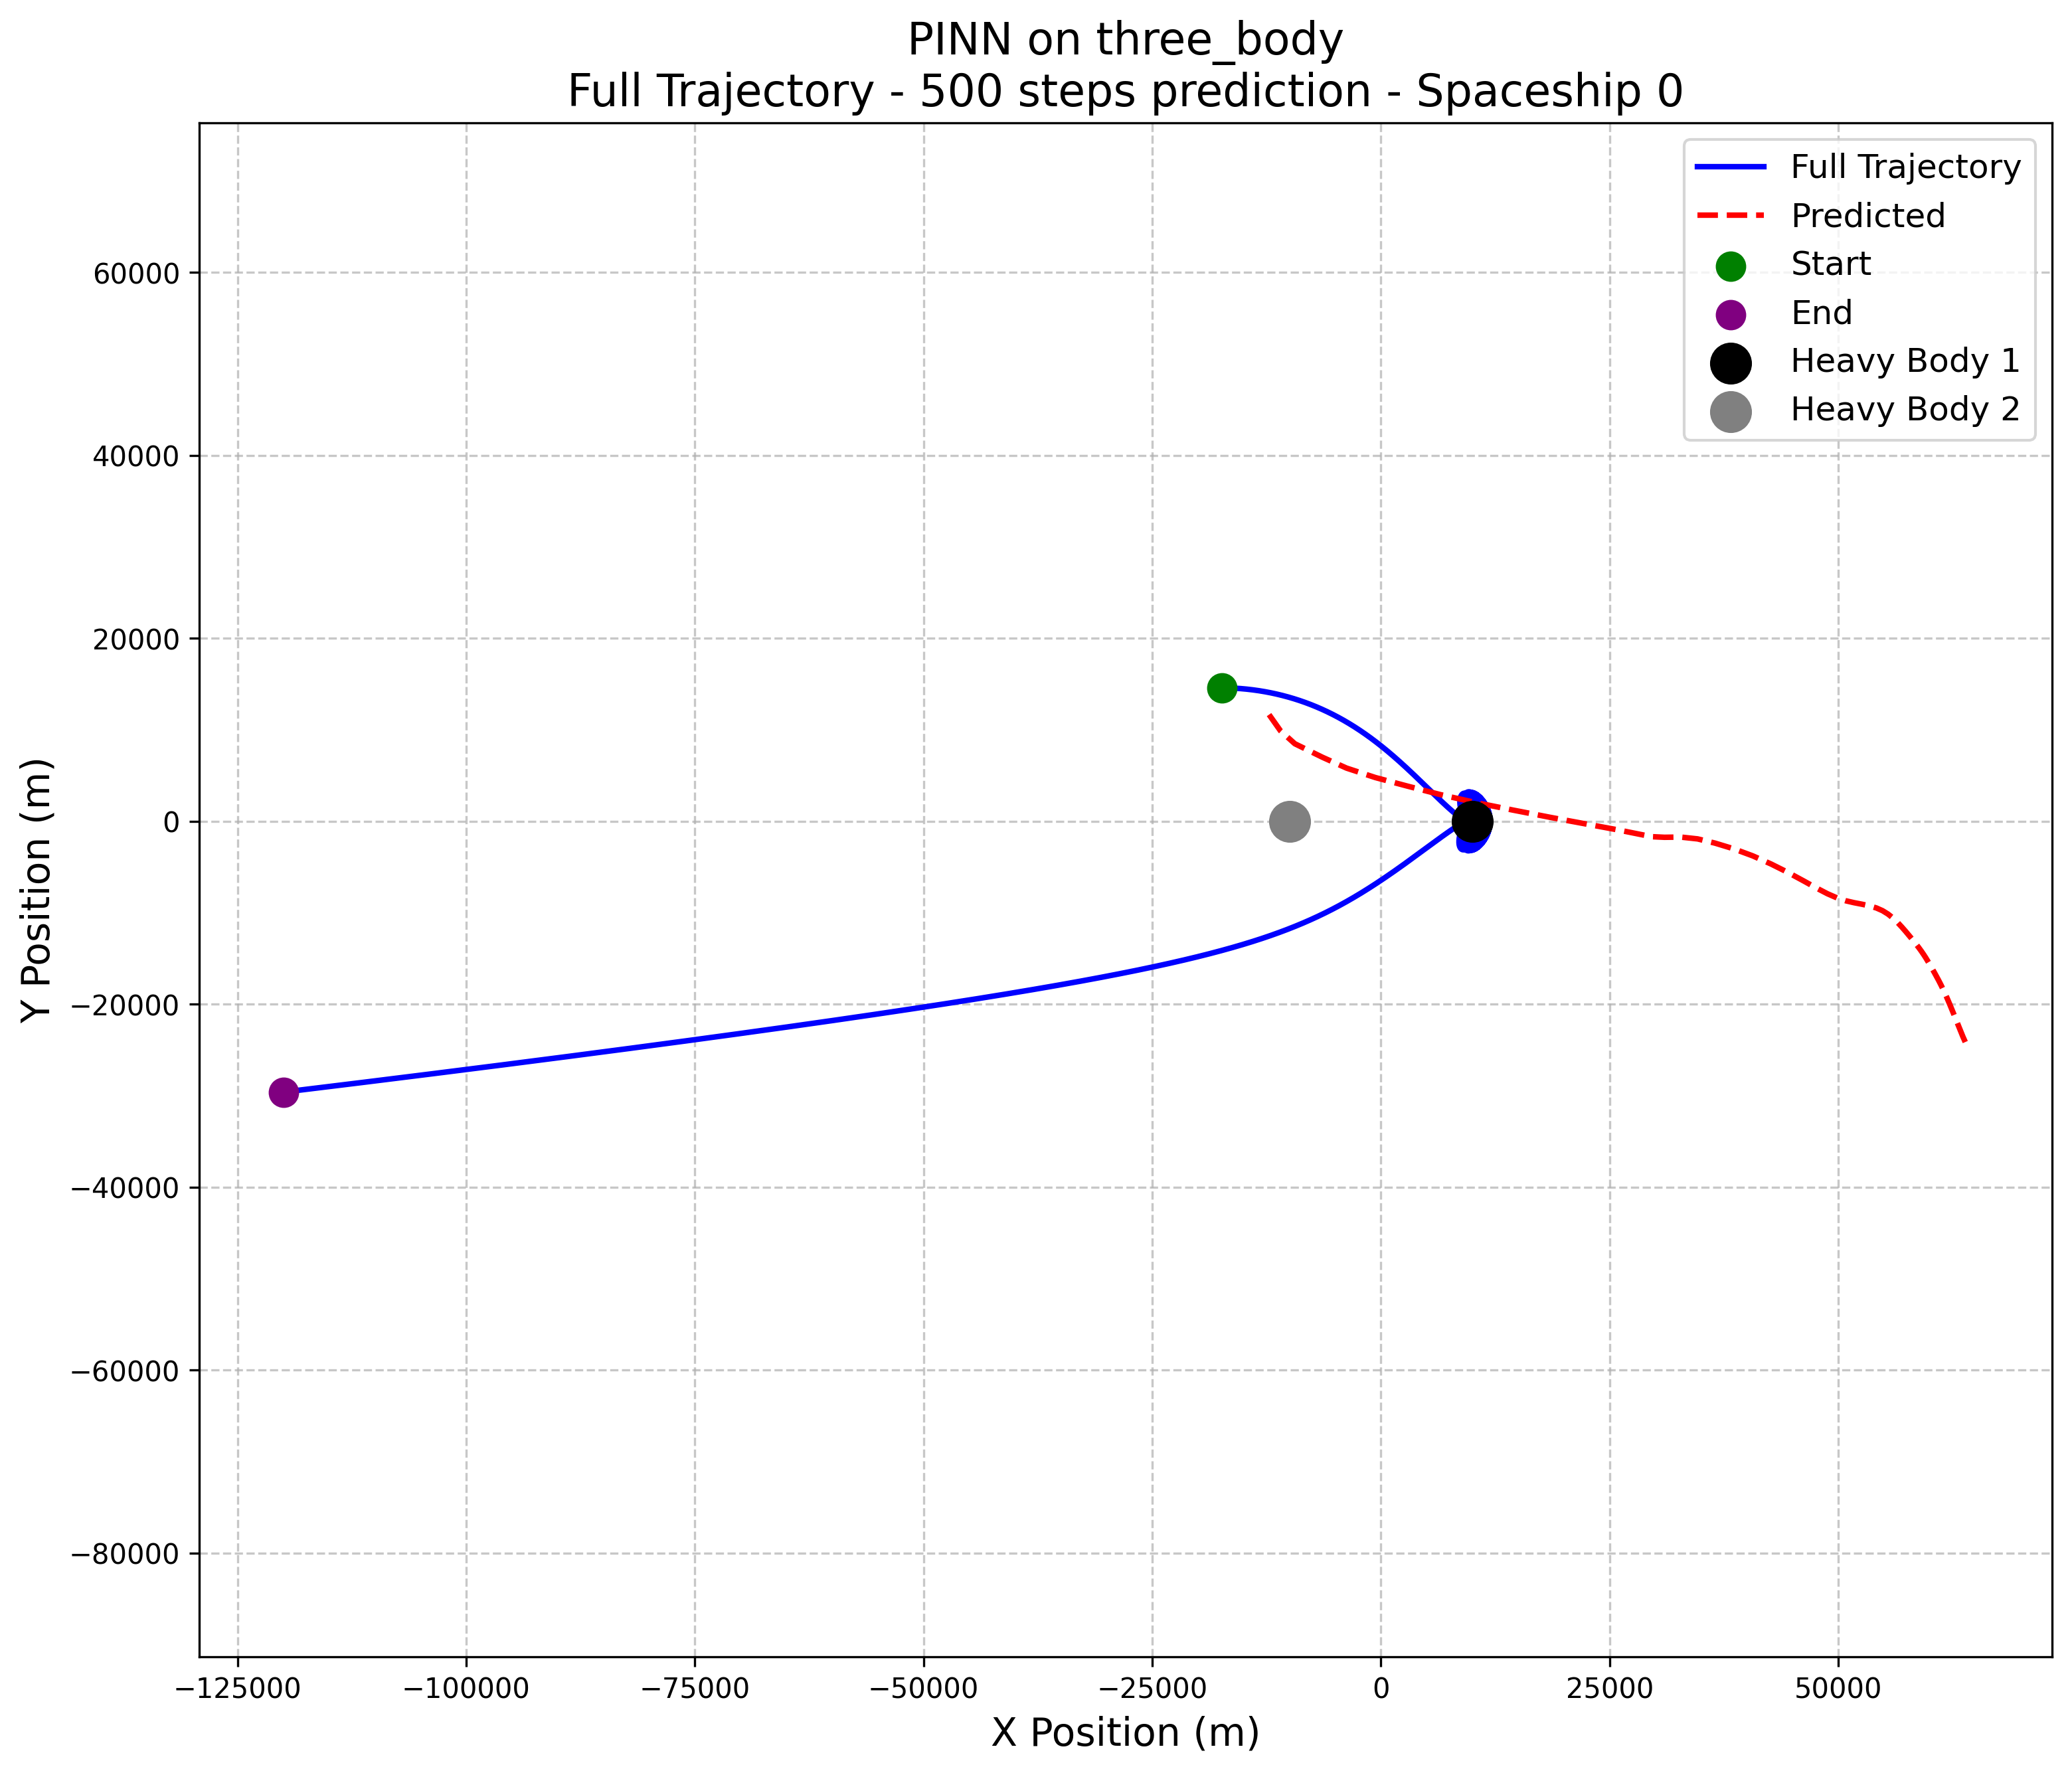
\includegraphics[width=0.27\textwidth]{../inference_results/val/PINN/three_body/500/full_trajectory_spaceship_0.png} &
      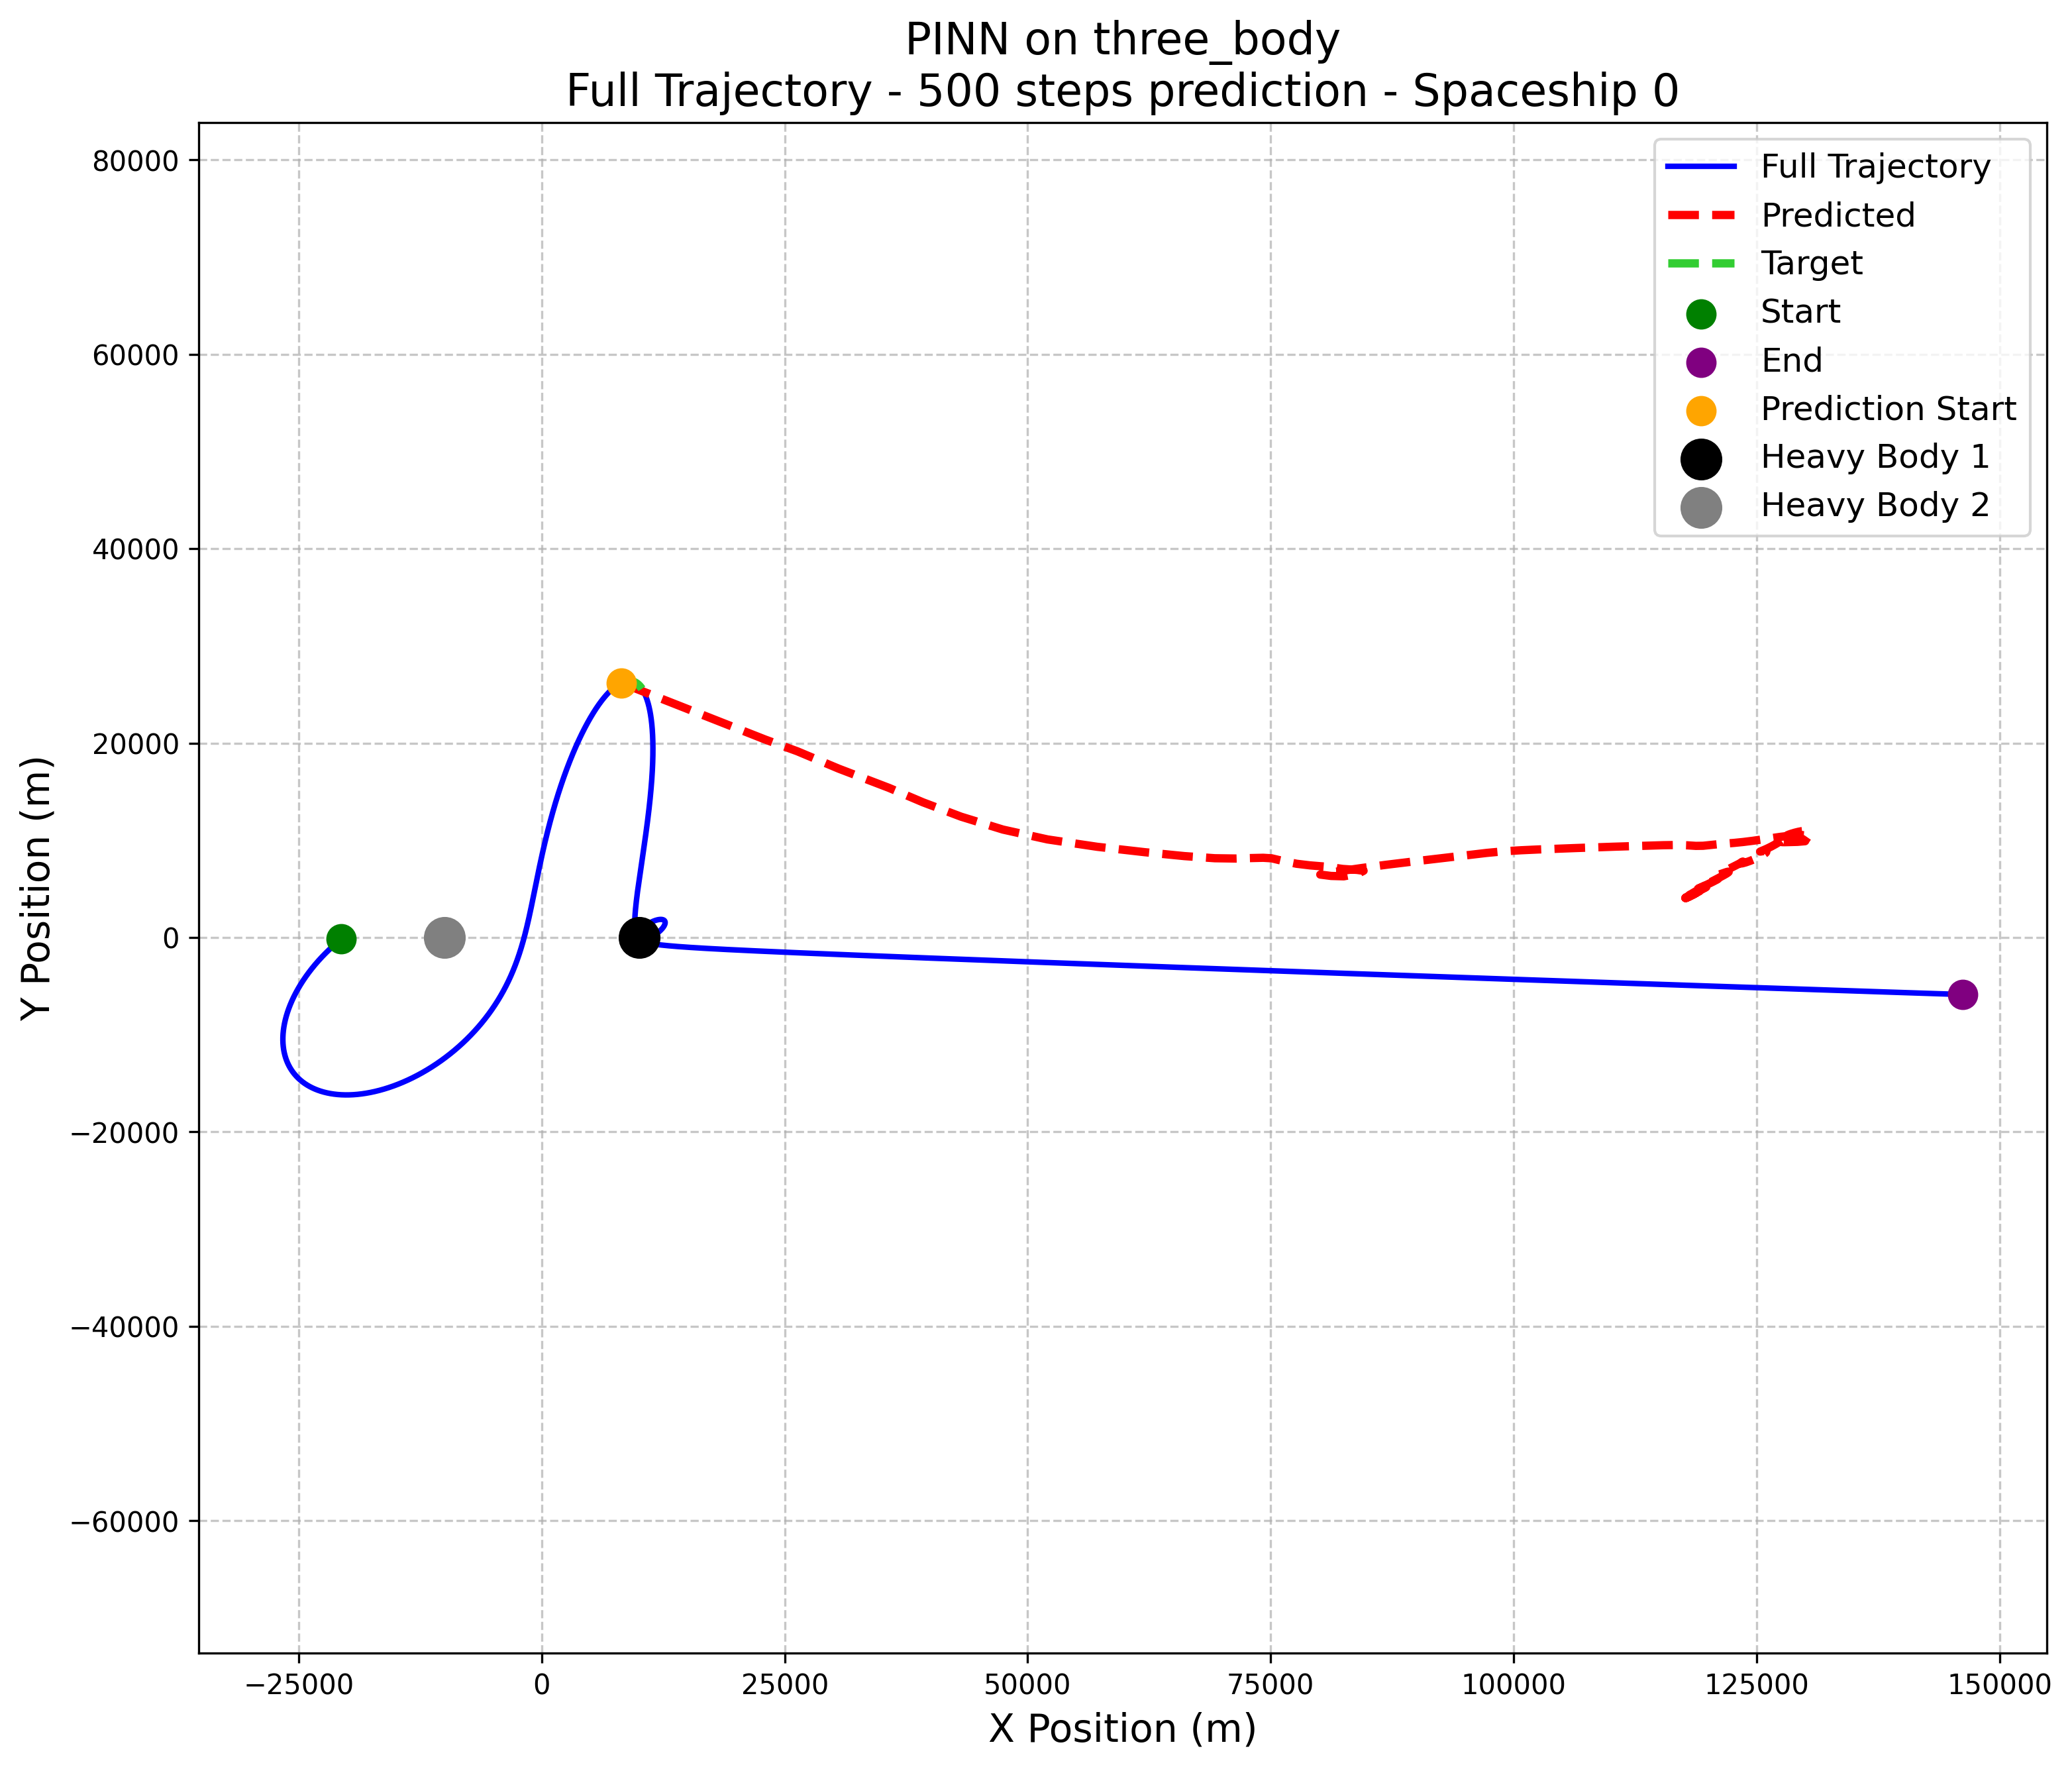
\includegraphics[width=0.27\textwidth]{../inference_results/test/PINN/three_body/500/full_trajectory_spaceship_0.png}
  \end{tabular}
\end{figure}
\end{document}
